% CREATED BY DAVID FRISK, 2018
% Title page and last page updated by Magnus Gustaver, 2020
% Updates in Settings and addition of Acronyms and Nomenclature templates by Kyriaki Antoniadou-Plytaria, 2021
% Updates for degree project report and chalmers/gu parameterization by Fredrik Albers, 2023


% IMPORT SETTINGS
\documentclass[12pt,a4paper,twoside,openright]{report}
% CREATED BY Kyriaki Antoniadou-Plytaria, 2021

% BASIC SETTINGS
\usepackage{moreverb}								% List settings
\usepackage{textcomp}								% Fonts, symbols etc.
\usepackage{lmodern}								% Latin modern font
\usepackage{helvet}									% Enables font switching
\usepackage[T1]{fontenc}							% Output settings
\usepackage[english]{babel}							% Language settings
\usepackage[utf8]{inputenc}							% Input settings
\usepackage{amsmath}								% Mathematical expressions (American mathematical society)
\usepackage{amssymb}								% Mathematical symbols (American mathematical society)
\usepackage{graphicx}								% Figures
\usepackage{subfig}									% Enables subfigures
\numberwithin{equation}{chapter}					% Numbering order for equations
\numberwithin{figure}{chapter}						% Numbering order for figures
\numberwithin{table}{chapter}						% Numbering order for tables
\usepackage{listings}								% Enables source code listings
\usepackage{chemfig}								% Chemical structures
\usepackage[top=3cm, bottom=3cm,
			inner=3cm, outer=3cm]{geometry}			% Page margin lengths			
\usepackage{eso-pic}								% Create cover page background
\newcommand{\backgroundpic}[3]{
	\put(#1,#2){
	\parbox[b][\paperheight]{\paperwidth}{
	\centering
	\includegraphics[width=\paperwidth,height=\paperheight,keepaspectratio]{#3}}}}
\usepackage{float} 									% Enables object position enforcement using [H]
\usepackage{parskip}								% Enables vertical spaces correctly 

% DEFINE THESIS TYPE
\def\ThesisType{M} % M - master, B - bachelor

% DEFINE INSTITUTION LOCATION
\def\InstitutionLocation{C} % C - Chalmers only, G - Chalmers and GU combined

% COLOR FOR HEADERS
\definecolor{headerBrown}{RGB}{144,102,78}
\if\ThesisType B
\definecolor{thesisHeaderColor}{RGB}{126,180,56} % Green
\fi
\if\ThesisType M
\definecolor{thesisHeaderColor}{cmyk}{0.14,0,0,0.65} % Gray
\fi

% OPTIONAL SETTINGS (DELETE OR COMMENT TO SUPRESS)

% Disable automatic indentation (equal to using \noindent)
\setlength{\parindent}{0cm}                         


% Caption settings (aligned left with bold name)
\usepackage[labelfont=bf, textfont=normal,
			justification=justified,
			singlelinecheck=false]{caption} 		

		  	
% Activate clickable links in table of contents  	
\usepackage{hyperref}								
\hypersetup{colorlinks, citecolor=black,
   		 	filecolor=black, linkcolor=black,
    		urlcolor=black}


% Define the number of section levels to be included in the t.o.c. and numbered	(3 is default)	
\setcounter{tocdepth}{5}							
\setcounter{secnumdepth}{5}	


% Chapter title settings
\usepackage{titlesec}		
\titleformat{\chapter}[display]
  {\Huge\bfseries\filcenter}
  {{\fontsize{50pt}{1em}\vspace{-4.2ex}\selectfont \textnormal{\thechapter}}}{1ex}{}[]


% Header and footer settings (Select TWOSIDE or ONESIDE layout below)
\usepackage{fancyhdr}								
\pagestyle{fancy}  
\renewcommand{\chaptermark}[1]{\markboth{\thechapter.\space#1}{}} 


% Select one-sided (1) or two-sided (2) page numbering
\def\layout{2}	% Choose 1 for one-sided or 2 for two-sided layout
% Conditional expression based on the layout choice
\ifnum\layout=2	% Two-sided
    \fancyhf{}			 						
	\fancyhead[LE,RO]{\nouppercase{ \leftmark}}
	\fancyfoot[LE,RO]{\thepage}
	\fancypagestyle{plain}{			% Redefine the plain page style
	\fancyhf{}
	\renewcommand{\headrulewidth}{0pt} 		
	\fancyfoot[LE,RO]{\thepage}}	
\else			% One-sided  	
  	\fancyhf{}					
	\fancyhead[C]{\nouppercase{ \leftmark}}
	\fancyfoot[C]{\thepage}
\fi


% Enable To-do notes
\usepackage[textsize=tiny]{todonotes}   % Include the option "disable" to hide all notes
\setlength{\marginparwidth}{2.5cm} 


% Supress warning from Texmaker about headheight
\setlength{\headheight}{15pt}		


% Tag command (invisible)
\newcommand{\tagtemp}{\textcolor{white}{, template by Kyriaki Antoniadou-Plytaria}}

% Allow a table to split
\usepackage{longtable}





\begin{document} 

% COVER PAGE, TITLE PAGE AND IMPRINT PAGE
\pagenumbering{roman}			% Roman numbering (starting with i (one)) until first main chapter
% CREATED BY MAGNUS GUSTAVER, 2020

\ifx\ThesisType\undefined
Undefined Thesis type in settings.tex
\else
  \if\ThesisType M
    \else
    \if\ThesisType B
    \else
    Define \textbackslash ThesisType as M for master's thesis or B for bachelor thesis in settings.tex
    \fi
  \fi
\fi

% COVER PAGE
\begin{titlepage}
\newgeometry{top=3cm, bottom=1cm,
			left=2.25 cm, right=2.25cm}	% Temporarily change margins		
			
%Header Front Page
\ifx\ThesisType\undefined
\else
    \vtop{
        \null\vspace{-25mm}
        
        \if\ThesisType M   %Defined in settings.tex
        \centerline{
\includegraphics[width=1.18\textwidth]{figure/auxiliary/GrayHeaderPattern.jpg}}
        \fi
        \if\ThesisType B
        \centerline{
\includegraphics[width=1.18\textwidth,height=80pt]{figure/auxiliary/GreenHeaderPattern.jpg}}
        \fi
        \vspace{-2.3cm}
        
        \if\InstitutionLocation C   %Defined in settings.tex
        \hbox{\hspace{0mm}
\includegraphics[height=18mm]{figure/auxiliary/AvancezChalmersU_white_right.eps}}
        \fi
        \if\InstitutionLocation G
        \vspace{2.5mm}
        \hbox{\hspace{0mm}
\includegraphics[height=13mm]{figure/auxiliary/chalmers_gu_white_eng.eps}}
        \vspace{2.5mm}
        \fi
        
        \centerline{\textcolor{headerBrown}{\rule{1.18\textwidth}{4pt}}}
        \vspace{\paperheight}\vspace{-85mm}
        \centerline{\textcolor{thesisHeaderColor}{\rule{1.1\textwidth}{0.8pt}}} % Rule after Department
        \vspace{-\paperheight}\vspace{85mm}
    }
\fi

% Cover picture (replace with your own or delete)		
% \begin{figure}[H]
% \centering
% \vspace{1cm}	% Adjust vertical spacing here
% 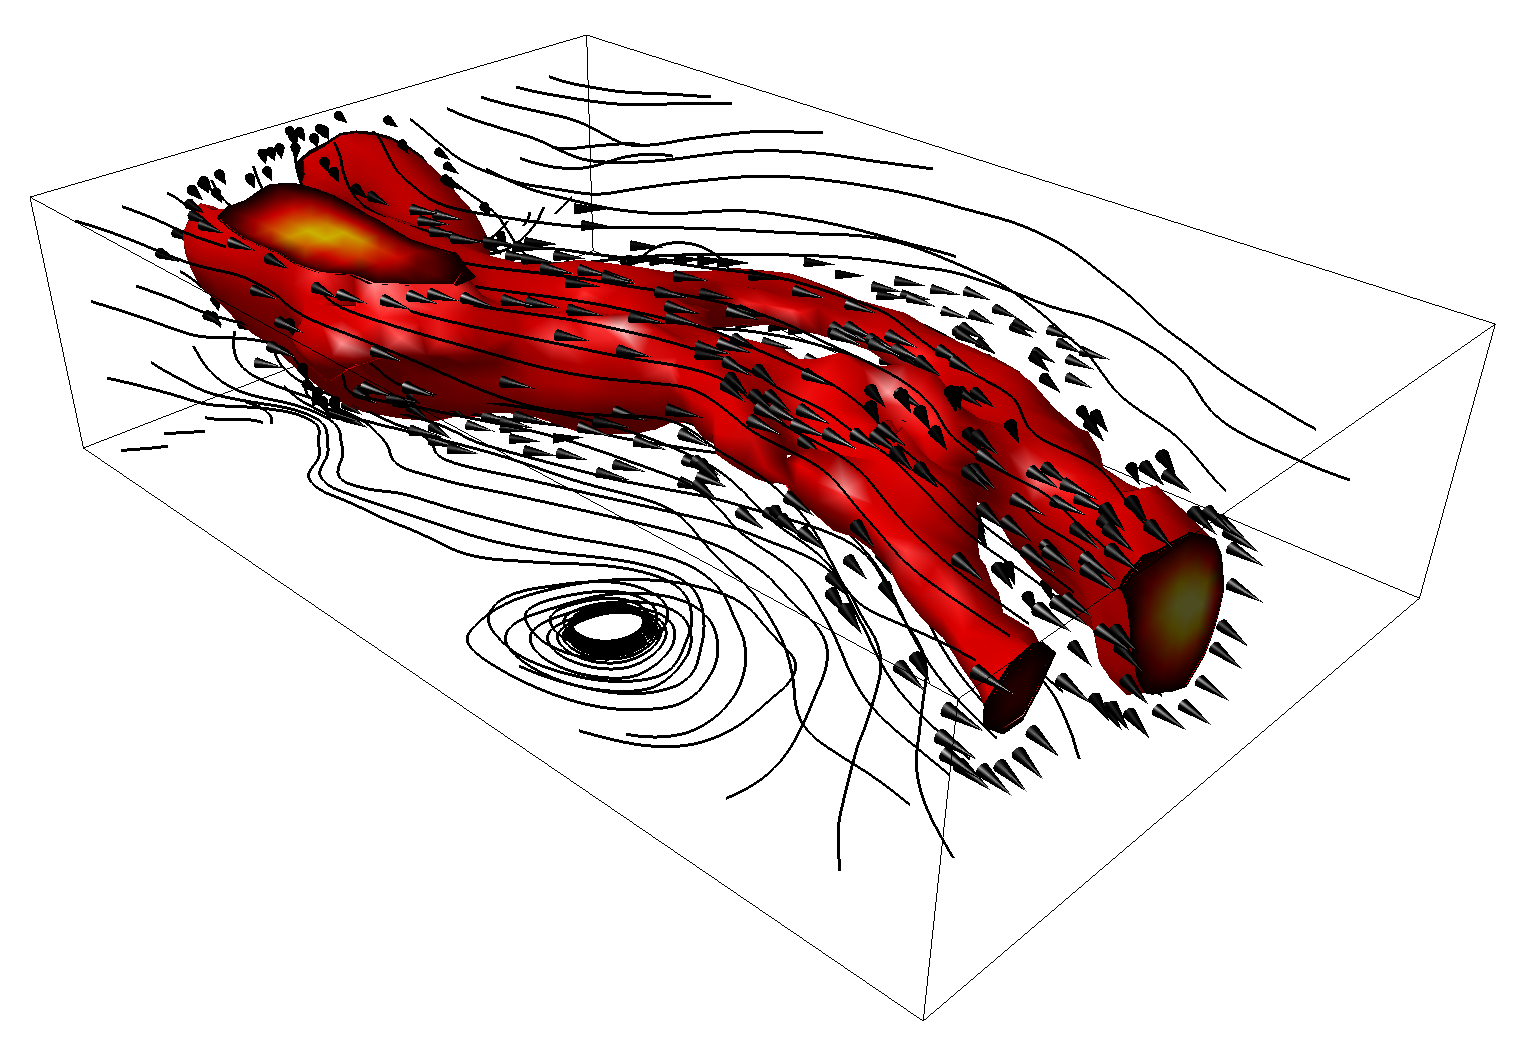
\includegraphics[width=0.9\linewidth]{figure/Wind.png}
% \end{figure}

% Cover text
\mbox{}
\vfill
\renewcommand{\familydefault}{\sfdefault} \normalfont % Set cover page font
\textbf{{\Huge 	Antibiotic Resistance Mutations in Aquatic Plastisphere Microbiomes}} 	\\[0.5cm]
Degree project report in Biotechnology \setlength{\parskip}{1cm}

\noindent
{\Large FELIX BLOMFELT} \setlength{\parskip}{1.5cm}

\noindent
\textcolor{thesisHeaderColor}{\small\textbf{DEPARTMENT OF LIFE SCIENCES}}
\setlength{\parskip}{1mm}

\textsc{Chalmers University of Technology} \\
{\small Gothenburg, Sweden \the\year \\
\href{www.chalmers.se}{www.chalmers.se}}\vspace{1.7cm}

\renewcommand{\familydefault}{\rmdefault} \normalfont % Reset standard font
\end{titlepage}


% BACK OF COVER PAGE (BLANK PAGE)
\newpage
\restoregeometry
\thispagestyle{empty}
\mbox{}


% TITLE PAGE
\newpage
\thispagestyle{empty}
\begin{center}
    \textsc{\large Degree project report \the\year}\\[4cm]
    \textbf{\Large Antibiotic Resistance Mutations in Aquatic Plastisphere Microbiomes} \\[1cm]
    {\large FELIX BLOMFELT}
    \vfill	
    % Logotype on titlepage	
    \begin{figure}[H]
        \centering
        % Remove this figure to remove the titlepage logotype
        \if\InstitutionLocation C   %Defined in settings.tex
        
\includegraphics[width=0.2\pdfpagewidth]{figure/auxiliary/AvancezChalmersU_black_centered.eps} \\
        \fi
        \if\InstitutionLocation G
        
\includegraphics[width=0.3\pdfpagewidth]{figure/auxiliary/chalmers_gu_black_centered_eng.eps} \\
        \fi
    \end{figure}
    \vspace{5mm}
    Department of Life Sciences \\
    \textsc{Chalmers University of Technology} \\
    \if\InstitutionLocation G
    \textsc{University of Gothenburg} \\
    \fi
    Gothenburg, Sweden \the\year \\
\end{center}


% IMPRINT PAGE (BACK OF TITLE PAGE)
\newpage
\thispagestyle{plain}
\vspace*{4.5cm}
Antibiotic Resistance Mutations in Aquatic Plastisphere Microbiomes\\
\\
FELIX BLOMFELT \setlength{\parskip}{1cm}

\copyright ~ FELIX BLOMFELT, \the\year. \setlength{\parskip}{1cm}

Supervisor: Máté Vass, Department of Life Sciences\\
Examiner: Johan Bengtsson Palme, Department of Life Sciences \setlength{\parskip}{1cm}

Degree project report \the\year\\	
Department of Life Sciences\\
Chalmers University of Technology\\
SE-412 96 Gothenburg\\
Sweden\\
Telephone +46 31 772 1000 \setlength{\parskip}{0.5cm}

\vfill
% Caption for cover page figure if used, possibly with reference to further information in the report
%Cover: Wind visualization constructed in Matlab showing a surface of constant wind speed along with streamlines of the flow. \setlength{\parskip}{0.5cm}

Typeset in \LaTeX \tagtemp\\
%Printed by Chalmers Reproservice\\
Gothenburg, Sweden \the\year


% ABSTRACT
\newpage
% CREATED BY MAGNUS GUSTAVER, 2020
Antibiotic Resistance Mutations in Aquatic Plastisphere Microbiomes\\
\\
FELIX BLOMFELT\\
Department of Life Sciences\\
Chalmers University of Technology\\
\if\InstitutionLocation G
University of Gothenburg\\
\fi
\setlength{\parskip}{0.5cm}

\thispagestyle{plain}			% Supress header 
\setlength{\parskip}{0pt plus 1.0pt}
\section*{Abstract}

% \begin{itemize}
    % \item ll - start/stop compiling the document, turns on auto compilation.
    % \item lk - stop compilation process. 
    % \item lc - clear auxiliary files 
    % \item lv - forward search, will open compiled pdf. Some pdf viewers support the ability to jump to the current location in the pdf. 
    % \item le - open/close quickfix window. Pressing enter on the error moves the cursor to the line containing the error. 
    % % TO-DO example of to-do-note, see also: 
    % \item todo{To create a visible todo-note}
    % \item lt - open table of contents for the file. Includes section, labels, references, and TODOs. 
    % \item [[, [], ][, ]] - move between section boundaries. 
    % \item { - move to previous empty line, } to the next. 
    % \item \% - move to next/matching bracket. 
    % \item ic - excludes the backslash of latex commands. 
    % \item ac - includes the backslash of latex commands. 
    % \item cse - change surrounding environment, e.g. align to equation. 
    % \item tsd - toggles between () and \( \left( \right) \) in enviroments.
    % \item tse - toggles the \* in enviroments.
    % \item c - change 
    % \item d - delete 
    % \item :help vimtex - open the help page
    % \item S - delete whole line and begin insert
    % \item s - delete character and begin insert
% 
% \end{itemize}
% 
% 
% \section{TODO}
% \begin{itemize}
    % \item Boxplots
        % \begin{itemize}
            % \item Samples
            % \item Mutations
            % \item Sampletype/substrate
            % \item Study and Coords - mention but no results?
            % \item Ecosystem - mention but no results?
        % \end{itemize}
    % \item[x] Wilcoxon test
        % \begin{itemize}
            % \item[x] Pseudo-mean
            % \item[x] Paired or not
        % \end{itemize}
    % \item[x] Random Forest
            % %\item "Permuting a useful variable, tend to give relatively large decrease in mean gini-gain. GINI importance is closely related to the local decision function, that random forest uses to select the best available split. Therefore, it does not take much extra time to compute. On the other hand, mean gini-gain in local splits, is not necessarily what is most useful to measure, in contrary to change of overall model performance. Gini importance is overall inferior to (permutation based) variable importance as it is relatively more biased, more unstable and tend to answer a more indirect question" - see https://stats.stackexchange.com/questions/197827/how-to-interpret-mean-decrease-in-accuracy-and-mean-decrease-gini-in-random-fore
    % \item Weird point-plot, see fig \ref{pointplot_mutations}
        % \subitem Use it or not? Kinda relevant
    % \item Taxonomic Composition - mention above after metaxaQR?
% \end{itemize}
% 
Antibiotic resistance, where pathogens are less susceptible to treatments with antibiotics, is one of the top threats to human health, and antibiotic resistance is estimated to have caused more than one million deaths in 2021. 
% Too large jump.
% Potentially start by talking about the pathogens and then mention that certain pathogens can be enriched greatly on the surface of microplastics
Pathogens such as \emph{Mycobacterium tubercolosis} can aquire mutations which confer antibiotic resistance to rifamycin, the most common treatment for infections with the pathogen. 
Human pathogens has been shown to be enriched on the surface of microplastics, and enrich the presence of antibiotic resistance genes (ARGs) in the microbes.
% Define knowledge gap

Previous studies have commonly looked only at the resistance genes present on microplastics, and not the specific point mutations which may confer resistances.
This work analyzes the metagenome of 395 samples from publically available data to identify point mutations, leading to antibiotic resistance. 
To comprehensively assess point mutation frequencies, the presence of ARGs on microplastics were compared with those found in the surrounding water, and other substrates.

The results suggest that plastics, in general, did not increase the presence of individual resistance-conferring point mutations compared to water,
%percentages!
however specific plastic substrates did carry bacteria with elevated point mutations, such as polyethylene-fiber (PF, +48\%), polyethylene-fiber-polyethylene (PFP, +140\%), polyvinyl chloride (PVC, +25\%), low-density polyethylene (LDPE, +52\%), Ecovio(+103\%), and BI-OPL(120\%). 
% percentages!

Specific substrates (HDPE, PBSA, PFP, PHA, PHBV) were identified by their point mutations of their microbiomes, conferring resistance to fluoroquinolone, rifamycin, aminocoumarin, and rifampicin.
Plastics as a general group had, however, no specific point mutations which would have distinguished it from the water samples, meaning that different plastic substrates induce different point mutations. 
The plastic group as a whole contained more different point mutations than the water group, but there was no increase in specific point mutations. 
This nonspecific increase in the overall level of point mutations could potentially be caused by oxidative stress from additives released from the microplastic particles during weathering and degradation processes, or pollutants adsorbed onto them.
%This work highlights the difference between different plastic substrates, and that care need to be taken to specify the plastic substrate used, since this can significantly impact the results.

This work highlights that several, but not all, plastic substrates increase the presence of specific point mutations and provide insights for further studies aimed at mitigating the impact of antibiotic resistance.

% KEYWORDS (MAXIMUM 10 WORDS)
\vfill
Keywords: antibiotic resistance, plastisphere, point mutations, AMR, ARG, aquatic ecosystems, bioinformatics, mumame.

\newpage				% Create empty back of side
\thispagestyle{empty}
\mbox{}


% ACKNOWLEDGEMENTS
\newpage
% CREATED BY MAGNUS GUSTAVER, 2020
\thispagestyle{plain}			% Supress header
\section*{Acknowledgements}

I would like to thank Johan Bengtsson Palme for welcoming me in his group, for the opportunity to work on this subject, and for his support during the project. 
I would also like to thank Máté Vass for his great help, guidance, and encouraging support during this project and the writing of this thesis. 
Additionally, I would like to thank C3SE for providing access to their computer cluster Vera for use during this project, as a part of project numbers C3SE 2025/1-11 \& NAISS 2025/6-76. 

% Text containing:
% \begin{itemize}
    % \item Thanks to: Johan, Máté, group.
    % \item Whoever is in charge of vera and the project number 
% \end{itemize}

\vspace{1.5cm}
\hfill
Felix Blomfelt, Gothenburg, May 2025

\newpage				% Create empty back of side
\thispagestyle{empty}
\mbox{}


% Acronyms
\newpage
\addcontentsline{toc}{chapter}{List of Acronyms}
\input{include/frontmatter/Acronyms}

% Nomenclature
\newpage
\addcontentsline{toc}{chapter}{Nomenclature}
% Created by Kyriaki Antoniadou-Plytaria, 2021
\thispagestyle{plain}			% Supress header

\chapter*{Nomenclature}
Below is the nomenclature of indices, sets, parameters, and variables that have been used throughout this thesis.
% \vspace*{-3cm}

\section*{Indices}
\renewcommand*{\arraystretch}{1.35}
\begin{longtable}{p{3cm}p{12cm}}
$i$,$j$ & Indices for distribution network buses\\
$t$ & Index for time step\\
\end{longtable}

% \vspace*{-3cm}
\section*{Sets}
\renewcommand*{\arraystretch}{1.35}
\begin{longtable}{p{3cm}p{12cm}}
$\mathcal{D}$ & Set of distribution network buses\\
$\mathcal{D}_{s}$ & Set of substation buses \\
$\mathcal{H}$ & Set of time steps (simulation/scheduling horizon)\\
$\mathcal{N}$ & Set of buses\\
\end{longtable}

\section*{Parameters}
% \vspace*{-3cm}
\renewcommand*{\arraystretch}{1.35}
\begin{longtable}{p{3cm}p{12cm}}
$\gamma$& Penalty coefficient\\
$\Delta t$& Time discretization step (time interval)\\
$\eta_{j}^{ch}$& Charging efficiency of BES\\
$\eta_{j}^{dis}$& Discharging efficiency of BES\\
$\boldsymbol{H}$& Adjacency matrix\\
$N$ & Number of iterations\\
$P_{j,t}^{L}$& Active power of load demand\\
$P_{j,t}^{PV}$& Active power from solar generation\\
\end{longtable}

\section*{Variables}
\renewcommand*{\arraystretch}{1.35}
\begin{longtable}{p{3cm}p{12cm}}
$p_{j}$& Active power injection at bus $j$\\
$p_{ji}$& Active power flow from bus $j$ to bus $i$\\
$v_{i}$ & Square of voltage magnitude at bus $i$\\

\end{longtable}

\renewcommand*{\arraystretch}{1}

% \newpage				% Create empty back of side
% \thispagestyle{empty}
% \mbox{}





% TABLE OF CONTENTS
\newpage
\tableofcontents

% OTHER FRONTMATTER
% List of figures (add to table of contents)
\cleardoublepage
\addcontentsline{toc}{chapter}{\listfigurename} 
\listoffigures
% List of tables (add to table of contents)
\cleardoublepage
\addcontentsline{toc}{chapter}{\listtablename}  
\listoftables


% START OF MAIN DOCUMENT
\cleardoublepage
\setcounter{page}{1}
\pagenumbering{arabic}			% Arabic numbering starting from 1 (one)
\setlength{\parskip}{0pt plus 1pt}

% INTRODUCTION
% CREATED BY MAGNUS GUSTAVER, 2020
\chapter{Introduction}

\section{Background}

\section{Purpose}

\section{Goals}

\section{Limitations / Demarcations}



% THEORY
% CREATED BY MAGNUS GUSTAVER, 2020
\chapter{Theory/Background}

% - sno källor ur introduction  of \cite{goswami2025MicroplasticsHiddenDrivers}
% - se också 2.3
% - många källor samma! Nästan alla metagenomic i table 1 har jag med.

% Introduction:
% Antibiotic resistance is one of the top threats to human health according to the WHO\cite{worldhealthorganization2023AntimicrobialResistance}, and bacterial antimicrobial resistance (AMR) is estimated to have caused 1.14 million deaths in 2021 \cite{naghavi2024GlobalBurdenBacterial}. 
% It is estimated that by the year 2050, resistant infections could be associated \todo{note ASSOCIATED with, only 1.91 million attributable to} with more than 8 million deaths anually\cite{naghavi2024GlobalBurdenBacterial}.
% 
% Pathogens can confer antibiotic resistance by %horizontal gene transfer (HGT) or 
% chromosomal mutations. 
% Microplastics have been shown to enrich potentially pathogenic bacteria that carry a great number of antibiotic resistance genes (ARGs)\cite{liu2021MicroplasticsAreHotspot, wu2019SelectiveEnrichmentBacterial}.
\todo{I feel like I have too little theory but I'm not sure what to include, what level to place it on. Include also: why point mutations? Why they are not studied more? Why antibiotic resistance is something good for the organims?}

\section{The plastisphere}
The plastisphere is a human-made ecosystem which consists of the microbial community which inhibit the surface of microplastics\cite{amaralzettler2020EcologyPlastisphere}. 
Microplastics are synthetic particles or polymeric matrices with a diameter between one micrometer and five millimetres, however the lower limit of this range is disputed\cite{frias2019MicroplasticsFindingConsensus}.
Approximately 5-13 million tonnes of plastic entered the ocean the year 2010, and is estimated to double by 2030\cite{amaralzettler2020EcologyPlastisphere}. In 2014 a total of 15-51 trillion microplastic particles was estimated to be present in the marine environment\cite{vansebille2015GlobalInventorySmall}.
Microplastics has been shown to release additives and accumulate other pollutants, as well as help transport them, increasing the oxidative stress of the organisms in the biofilm. These pollutants include heavy metals such as chromium and cadmium\cite{forero-lopez2022PlastisphereMicroplasticsSitu}.
The microbiome of the plastisphere is distinct from the microbiome of the surrounding water \cite{zadjelovic2023MicrobialHitchhikersHarbouring}, and has been shown to enrich ARGs compared to it\cite{zhou2024MicroplasticBiofilmsPromote}.

\section{Antibiotic resistance databases}
The antibiotic resistance database which is used in this study is release 4.0.0 of the the Comprehensive Antiobiotic Resistance Database (December 2024)\cite{alcock2023CARD2023Expanded}.
The database consists of manually curated entries which are labelled with at least four mandatory classification tags, which include \emph{AMR Gene Family}, \emph{Drug Class}, \emph{Resistance Mechanism}, and \emph{Antibiotic}\cite{alcock2020CARD2020Antibiotic}. 
The tag AMR Gene Family is of special interest, since it is the most granular of the tags and enables grouping of the point mutations based on their conferred resistance as well as the gene in which it is located, for example "rifampicin resistant rpoC". 
CARD is well-suited to use when researching mutations conferring resistance, compared to the National Database of Antibiotic Resistant Organisms (NDARO)\cite{feldgarden2021AMRFinderPlusReferenceGene} which would be well-suited for comparing acquired resistance genes through HGT. Both CARD and NDARO contain information on both acquired resistance genes and AMR associated mutations. 
\todo{Talk about how antibiotic resistance works, why is good for the organism?}
% - mention what is in it
% - Mention what is used
% - Mention what AMR Gene Family is

% \section{ARG Databases}
% CARD good for this: \cite{papp2022ReviewComparisonAntimicrobial}
% Contain list of snps.
% Contain list of WT sequences.
% Protein sequences listed.

% Other databases? see \emph{papp2022ReviewComparisonAntimicrobial}?

\section{Limitations and advantages of metagenomic data}
% - Shotgun metagenomics
%In order to detect the ARGs the metagenomic data was extracted, in their originals studies.
Metagenomic data is commonly collected through shotgun sequencing, an untargeted sequencing of all microbial genomes in the sample\cite{quince2017ShotgunMetagenomicsSampling}.
First, DNA is extracted from all the cells in the sample, then sheared into short DNA sequences called reads, which are then sequenced independently\cite{sharpton2014IntroductionAnalysisShotgun}. 
This enables the study of both the taxonomy of the samples, since some reads will match to the 16S region, a taxonomically relevant loci in bacteria and archea, and some will match the coding sequences of the microorganisms in the sample. 
The downside to this method is that it requires a large amount of data, since the metagenome of a sample is large and complex. 
%This complicates the analysis and makes the sequencing more expensive, but these problems are reduced by advancements in sequencing and computing technology. 
Metagenomic sequencing is preferred in this study rather than amplicon sequencing, which also extract the DNA from all cells of a sample but instead targets only a small taxonomically informative loci such as the 16S region in bacteria and archea. 
%Metagenomic sequencing may be compared to amplicon sequencing, which also extract the DNA from all cells of a sample, but instead targets only a small taxonomically informative loci such as the 16S region in bacteria and archea. 
It then amplifies the region using PCR, and therefore reduce the amount of sample needed for the analysis.
The amplicon sequencing method is therefore more suitable for the analysis of the diversity of the sample, and not to study the specific point mutations present in the metagenome of a sample.

%all the microbiomes are subject to untargeted sequencing

% \cite{quince2017ShotgunMetagenomicsSampling}
% High-throughput sequencing has enabled
% Metagenomic data
% - Shotgun sequencing
  % "untargeted sequencing of all microbial genomes in a sample"
  % can be used to profile taxonomic composition and functional potential of microbial communities

% \cite{sharpton2014IntroductionAnalysisShotgun}
% - Compare to amplicon, uses PCR -> has some biases associated with it
    % - can produce varying estimates of diversity, different loci  have differential power at resolving taxa. 
    % - typically only provides insight into taxonomic composition of the microbial community.
% 
% Shotgun: 
% - DNA extracted from all cells in a sample
% - all DNA is subsequently sheared into tiny fragments that are independently sequenced
% - this results in DNA sequences (reads) that align to various genomic locations for the myriad genomes present in the sample, including non-microbes.
% - Some of these reads will be sampled from taxonomically informative genomic loci (i.e. 16S), and others will be sampled from coding sequences that provide insight into the biological functions encoded in the genome.
% - provides the opportunity to simultaneously explore two aspects of a microbial community: who is there and what are they capable of doing. 
% 
% Challenges:
% - Relatively complex and large 
  % -> require large amount of data to identify meaningful results. (MuMaMe authors recommend X to achieve X, add amount in result?) 
% - May contain unwanted host DNA -> not a problem? microbiota
% - while contamination is a challenge general to environmental sequecning studies, the identification and removal of metagenomic sequence contaminants is especially problematic. 
  % -> For example, it can be difficult to determine which reads were generated from a detected contaminant's genome
  % -> A metagenomic contaminant can mislead analyses of community genetic diversity if the contaminant's genome is enriched for genes taht are uncommon in the community
% - Tend to be relatively expensive compared to amplicon

% - Compare to amplicon sequencing, see \cite{sharpton2014IntroductionAnalysisShotgun} but OLD?


% TODO: more in theory?
%\section{Mutation detection methods}
%There are multiple methods to detect mutations in metagenomic data, where one example is to
% todo M: For theory I guess you can focus on mutation-detection methods, arg databases, limitation and advantages of metagenomic data in general
% - Mutation detection methods
%   - Shotgun metagenomics -> MuMaMe needs 
% - ARG Databases
% - Limitation and advantages of metagenomic data in general

% 
% Mumame (magesh2019)
% Mumame is not aiming to find strain-level differences in taxonomic composition, thus enabling it to operate at much lower sequencing depths as complete coverage of the targeted genomes is not necessary for the analysis.Mumame is not aiming to find strain-level differences in taxonomic composition, thus enabling it to operate at much lower sequencing depths as complete coverage of the targeted genomes is not necessary for the analysis.Mumame is not aiming to find strain-level differences in taxonomic composition, thus enabling it to operate at much lower sequencing depths as complete coverage of the targeted genomes is not necessary for the analysis.
% From figure 2B in it: the proportion of reads with mutation must be ~25% in order to be detected as significant


% METHODS
% CREATED BY MAGNUS GUSTAVER, 2020
\chapter{Methods}
% All methods used:
% Download Data: 
% - bash: ena browser
% Pipeline 1:
% Annotation Pipeline:
% - TrimGalore! - Trims
%   - MultiQC - Generates a report of the trim-results (it's own pipeline but eh)
% - MetaxaQR - Annotation? SSU/LSU
%   - MetaxaQR_ttt - Taxonomic traversal tool - outputs number of identified SSU/LSU sequences associated with eac node in the taxonomic tree, at different levels (roughly corresponding to kingdoms, phyla, classes, orders, families, genera, species, subspecies, et.c. (We only use first six, down to ~Genus).
%   - MetaxaQR_dc - Data Collector - merges the output of several *.level_X.txt files from _ttt into one large abundance matrix.
% - Diamond - Not used?
%   - Gene Normalization - Not used?
% Create_DB Pipeline:
% - Build_resfinder_db: Only used for Diamond?
% - Build_mobileOG_db: Only used for Diamond?
% 
% Stuff done: 
% - TrimGalore! - Trims - version v0.12.2
%   trim_galore --paired -e 0.1 -j ${task.cpus} --phred33 -q 28 --fastqc ${reads[0]} ${reads[1]}
%   - MultiQC - Generates a report of the trim-results (it's own pipeline but eh) - version 1.18 
%     multiqc -f ${params.trimgalore_path}*fastqc.zip
% - MetaxaQR - Annotation? SSU/LSU - version 3.0 b3
%   metaxaQR -1 read_R1.fastq -2 read_R2.fastq -o ${sample_id}_${params.run_id} --cpu ${task.cpus} -g SSU -d /MetaxaQR/metaxaQR_db/SSU/mqr
%   - MetaxaQR_ttt - Taxonomic traversal tool - outputs number of identified SSU/LSU sequences associated with eac node in the taxonomic tree, at different levels (roughly corresponding to kingdoms, phyla, classes, orders, families, genera, species, subspecies, et.c. (We only use first six, down to ~Genus).
%    metaxaQR_ttt -i ${genus_files} -o ${sample_id}_${params.run_id}  -m 6
%   - MetaxaQR_dc - Data Collector - merges the output of several *.level_X.txt files from _ttt into one large abundance matrix.
%     metaxaQR_dc *.level_6.txt
%
% LaTeX:
% - Boxplots
% - Wilcoxon test
% - Microeco
%   - LEfSe - Not used?
%   - RandomForest

% Other things to mention in method
% - Where data is from
% - CARD
% - Number of samples of each type

% VERSION AV PROGRAMMET BROR, se ovan
% Options? in brackets?

\section{Data Processing}
The studies containing the metagenomic data used in this study were identified in the Nucleotide database of the National Center for Biotechnology Information using the search terms \emph{"shotgun metagenomics plastisphere microbiome", "(plastisphere metagenome shotgun) NOT MAG"}, and \emph{"txid1342751[Organism:noexp] NOT 16S NOT amplicon"}. The BioProject accession number was then used to download the metagenomic data from each dataset from the European Nucleotide Archive (ENA) at EMBL-EBI \cite{embl-ebi2025ENABrowser}. 

Only studies that analysed the metagenome in plastic and water substrates, and published their data in the ENA, were included. Some of them studied non-plastic substrates, however this was not a requirement for inclusion. Studies analysing wastewater were included in order to include samples which should be distinctly different from the water samples, since previous studies have shown that wastewater contributes to antimicrobial resistance \cite{sambaza2023ContributionWastewaterAntimicrobial}.

The full list of 16 studies are listed in Appendix \ref{appendix:studies}, and the full list of samples is available in \ref{appendix:samples}. All except one study were published between 2021 - 2025.
%In each study only the data from metagenomic analyses was included, the full list of samples are listed in appendix \ref{appendix:samples}.

A total of 395 samples from 53 different locations were analysed in this study (Figure \ref{world_map}). 
Samples were collected from the Pacific Ocean, along the east coast of the United States, in Europe, Australia, Japan, and China.

%\todo{M: Explain why these studies were kept for analyses. Think about the substrates and explain your reasonings.}
%\todo{mention that collected data from various ecosystems, which all had different substrates.}

\begin{figure}[h]
    \centering
    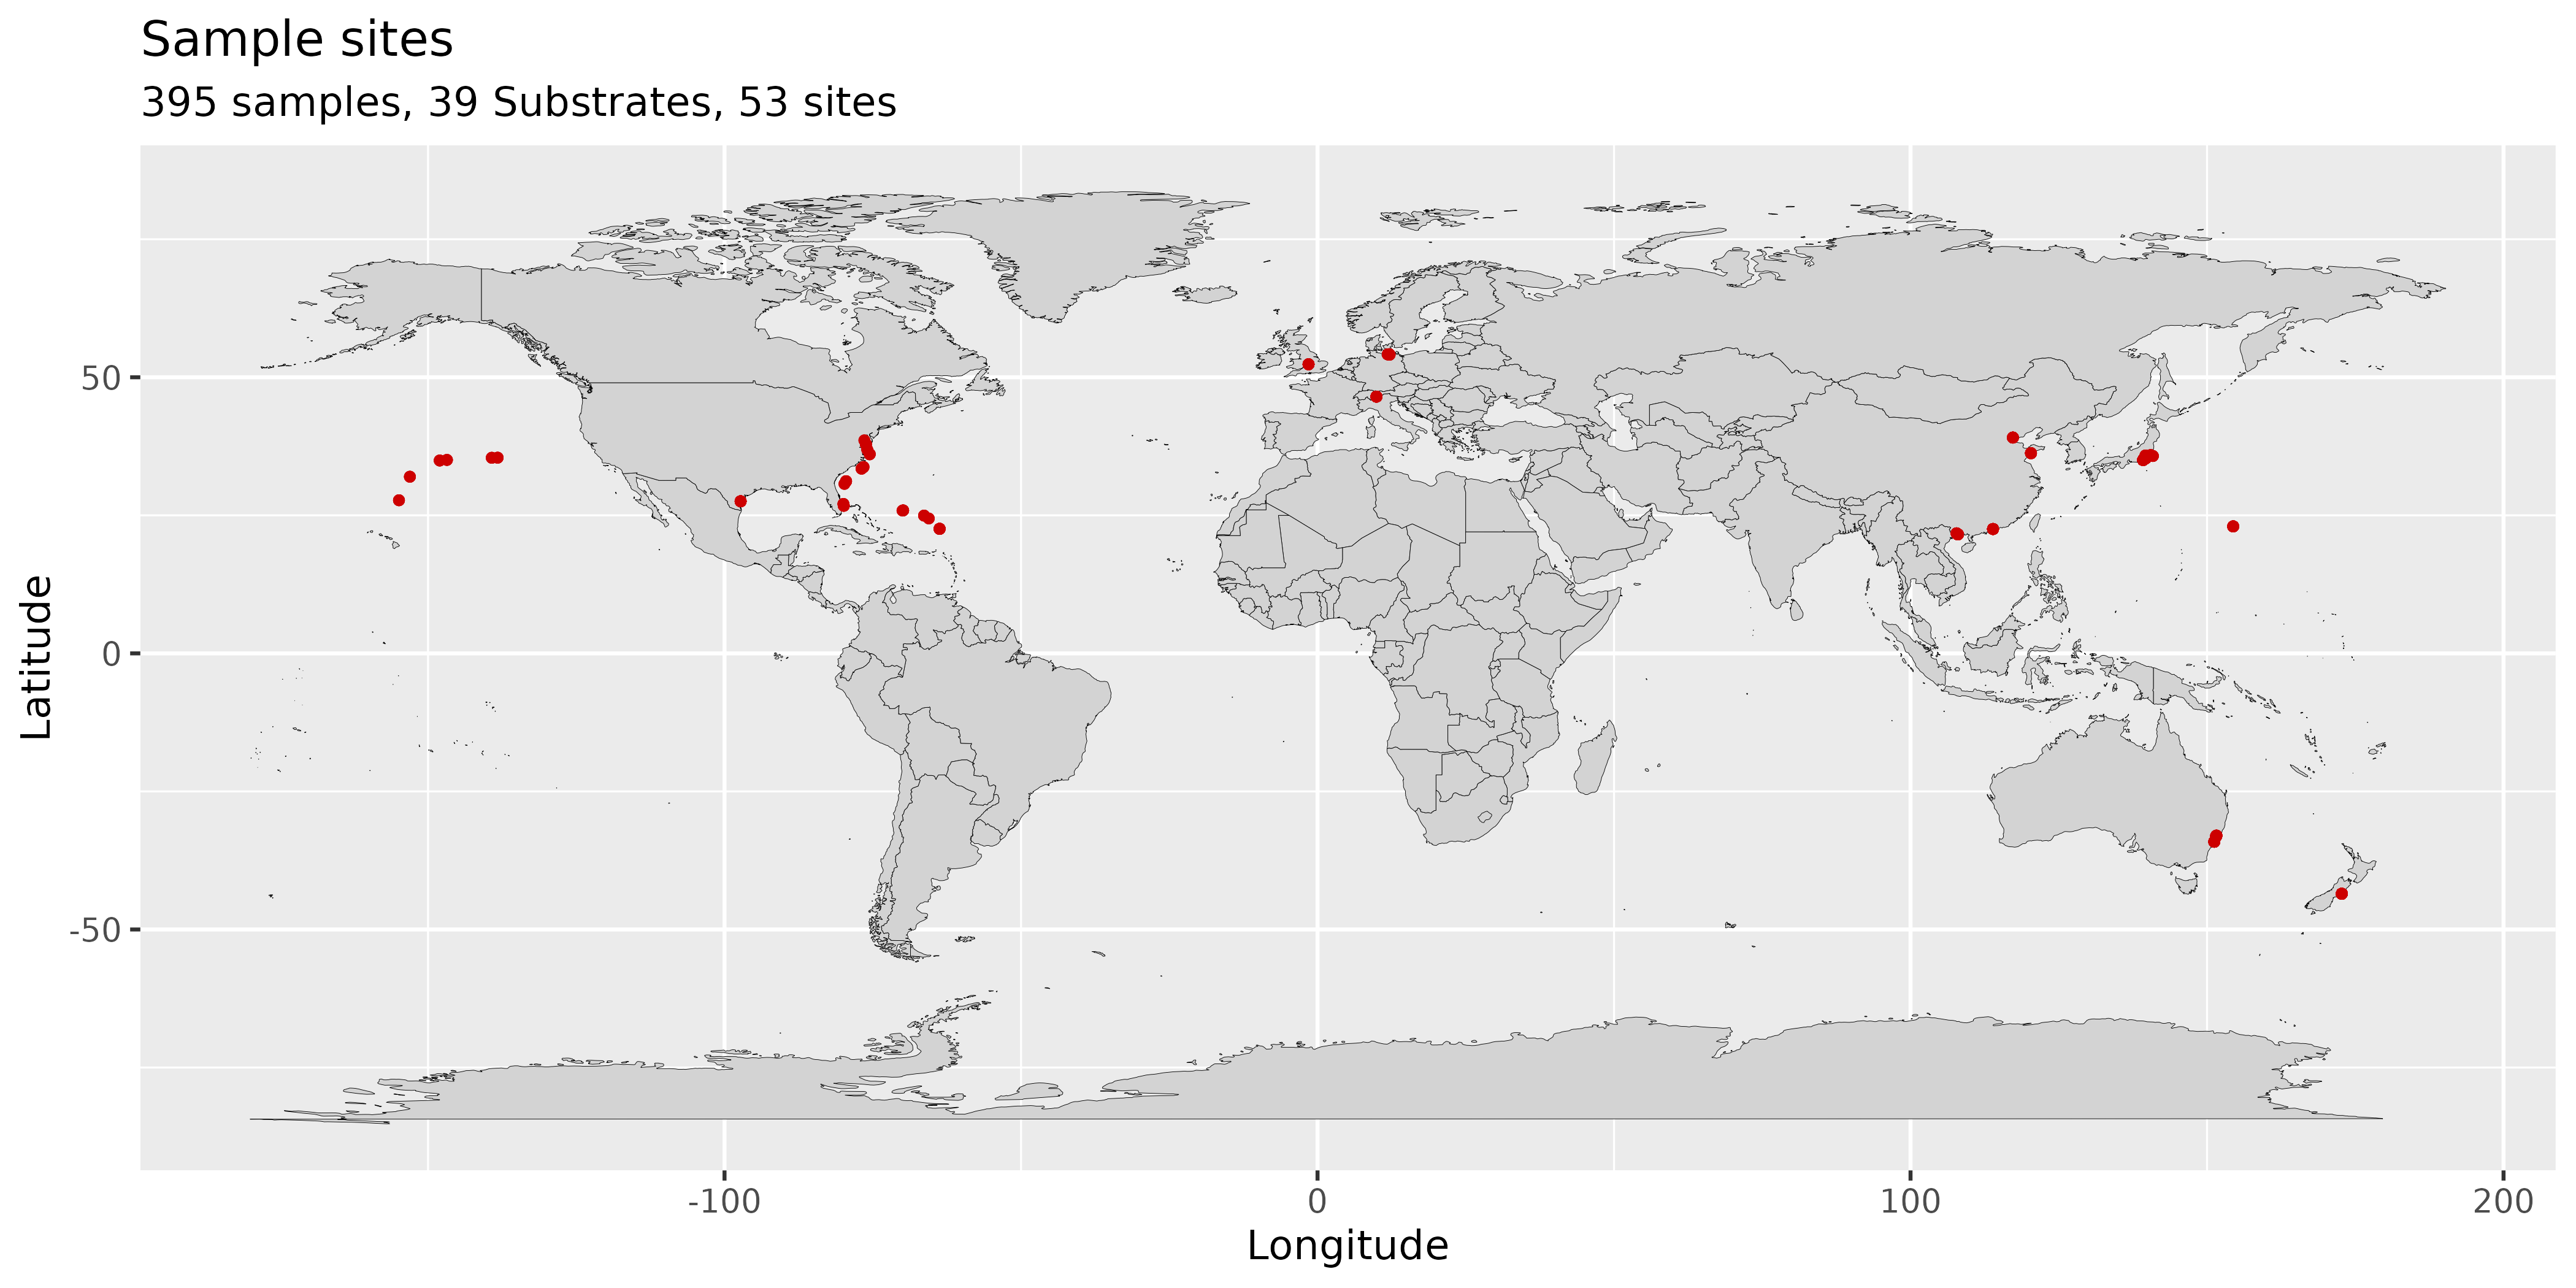
\includegraphics[width = \textwidth]{figure/map.png}
    \caption{Map showing the location of all samples in red}
    \label{world_map}
\end{figure}

The samples were divided into three groups, based on their substrate type as shown in table \ref{substrate_sampletype}. 
The water group included freshwater, seawater, and wastewater samples, the plastic group included 25 different plastics, and the non-plastic group consisted of seven different substrates, such as glass, wood, and soil. 
Each sample was also assigned an ecosystem type of either Ocean, Brackish, River, Wastewater, or Soil, based on the reported sample location.
Two substrates were included which are biodegradable plastic films, Ecovio and BI-OPL, both of which are blends of PBAT and PLA \cite{ruthi2023PlastisphereMicrobiomeAlpine}.

% \todo{M: this is just one part. Add also that this pipeline was used in order to get taxonomic information as well:} 

An in-house pipeline \cite{wenne2025Pipeline1} was used to trim and filter the data to remove low-quality reads, as well as annotate and map the sequences to databases in order to obtain taxonomic information about the samples.
%In order to trim the reads, filter the data to remove low-quality reads as well as annotate the genomes, an in house pipeline was used\cite{wenne2025Pipeline1}.
To filter the reads TrimGalore (v.0.12.2) \cite{krueger2023TrimGalore0122} was used, which does adapter and quality trimming. It uses FastQC for the quality filtering and Cutadapt for the adapter removal.
The result of the trimming was checked by visualizing the output of the trimming and filtering step using MultiQC \cite{ewels2016MultiQCSummarizeAnalysis}, which outputs an html file containing summarized results for all the samples. 

% --paired - performs length trimming of quality/adaper trimmed reads for paired-end files. 
           % To pass the validation test, both sequences of a pair are required to have minimum length defined.
% -e 0.1 - error rate of 0.1, number of errors divided by length of matching region. DEFAULT
% --phred33 - uses ASCII+33 quality scores as phred scores. DEFAULT
% -q 28 - Trim low-quality ends from reads in addition to adapter removal. Minimum quality of 28.
% --fastqc - Run fastQC in default mode on the fastq file once trimming is done.
A total of 379 samples were further analysed after the trimming, filtering and annotation pipeline.  
Of the original 395 samples, twelve were removed from further analysis since they contained less than three million reads, and four samples were removed since they belonged to substrates with less than three samples in total.
The mean amount of reads were approximately 25 million for the plastic group and 29 million for the water and non-plastic groups.


After the trimming and filtering step, the remaining reads were annotated using MetaxaQR (v. 3.0 b3) \cite{bengtsson-palme2015Metaxa2Improved}. This tool screens the input sequences for conserved regions of the SSU/LSU gene using hidden Markov models. These models are based on rRNA sequences from the SILVA database \cite{quast2012SILVARibosomalRNA}.
    A search using vmatch \cite{kurtzVmatchLargeScale} was then done on the sequences which are found to contain rRNA genes, against a specialized database crafted by the creators of MetaxaQR from release 138 of the SILVA database \cite{bengtsson-palmeMetaxaQRFAQMicrobiologyse}.% and release ten of Mitozoa\cite{donoriodemeo2012MitoZoa20Database}.
The taxonomic annotations are then collected by MetaxaQR Taxonomic Traversal Tool and MetaxaQR Data Collector, which finally outputs one large abundance matrix containing the results from all samples down to the genus level. 

In order to idenify the point mutations present in the samples, the tool MuMaMe (v. 1.0b) \cite{magesh2019MumameSoftwareTool} was used. MuMaMe consists of two tools, MuMaMe\_build and MuMaMe. 
The first tool builds a database of point mutations based on the Comprehensive Antibiotic Resistance Database (CARD) \cite{alcock2023CARD2023Expanded}. In this study the latest version (4.0.0) of CARD was used, which was released in December of 2024.
MuMaMe\_build uses a FASTA sequence file (protein\_fasta\_protein\_variant\_model.fasta) and a list of mutations (snps.txt) to extract sequence excerpts from the FASTA file. It creates one reference version, a version which does not confer resistance to the antibiotic, and at least one mutated version of the sequence, which potentially confer resistance. 
If there are several possible mutations close to each other it creates every possible combination of these mutations in addition to the reference version. 
The default value, which was used, is to extract 20 residues upstream and downstream of the mutation. 
A maximum depth of 16 was used instead of the default 12. This value limits the maximum amount of mutations that are combined to create the database entries, 
meaning that if there are sufficiently many mutations close to each other not all possible combinations of these will be included in the database.

MuMaMe uses the database created by MuMaMe\_build and a FASTQ file, which in this study was the trimmed, filtered and validated files from TrimGalore. MuMaMe auto-detects the other file of the paired-end read and uses both at the same time. It uses usearch \cite{edgar2010SearchClusteringOrders} to map each sequence in the input files to a sequence in the database. Using a best-hit strategy, it can assign the read to either a reference sequence or a mutated sequence with higher certainty, since the entries in the database it built will contain both versions of every sequence.
MuMaMe outputs a matrix with the number of reads mapped to the mutated and reference version of each point mutation, from each sample.
%This file was then used in further analysis in a Jupyter Notebook, available on \href{to do? add link to notebook}{GitHub} 

%\section{Jupyter Notebook}
% In the jupyter notebook, additional files will be used in combination with the results from MuMaMe. These include snps.txt and aro-index.tsv from the CARD\{weird}, as well as a tsv-file containing metadata for all the samples. The first two will be used to label the point mutations with their corresponding resistance mechanism, drug class and AMR gene family, while the last will be used to label the samples.
% 
% The CARD contain some duplicates, which come from different sources. We are not interested in this distinction so only the first one is kept. 

% Additionally, CARD contain some mis-labellings, which mean that some mutation positions seem to be written to occur outside the gene region.
% This issue stems from that the wrong sequence was added to the database in one case and that the original publication of the other mutations published nucleotide substitutions, which got mistaken for amino acid substitutions.
% The curators of the database are aware of this issue\cite{alcockLengthDiscrepancyProtein}.
% MuMaMe is unable to handle these erroneous positions and discards them.
% 
% Some mutations can't be labelled by the metadata, since they are not present in CARD in the unique combination which was found in the sample. 
% For example, if the mutations A12D and Y16S are present in CARD individually, but the combination of them was found in a sample. In these cases the metadata for another mutation in the same gene was used, which may be justified by them sharing the same accession number in the database. \todo{Förklara bättre? Att det är andra mutationer i samma gen som har samma accession?}
% \todo{Göra något med accession = 1, eller bara skippa det?}
% For example, if the above mutations are marked as being mutations in "Mycobacterium tuberculosis embC mutant conferring resistance to ethambutol", they get the same accession number as the other mutations with the same description. 
% The mutations for which labelling of this kind was done, was later assigned an accession number of 1 instead of their usual accesssion number, in order to be identified, but otherwise not disturb the analysis. 
%todo{En mutation utan någon annan liknande? Oklart var den fanns, hitta den? Tror löst?}

%todo{MOVE BOXPLOTS in code to above randomForest?}

\section{Statistical analysis}
The statistical analysis was done in R, all the code is available in appendix \ref{appendix:code}.

The number of reads which map to each point mutation that confer antibiotic resistance, was used to identify the overall mutation frequency of the sample. This value was divided by the total number of reads in the sample to normalize, in order to be able to compare between samples.

The other statistical analyses are based on the relative mutation frequency, where the number of reads matched to the mutated version of the gene is divided by the number of matches to the reference version of the gene.
This was done in order to analyse the frequency of mutation of each individual point mutation, and be able to compare between mutations with high and low amounts of reads mapped to them.
MuMaMe outputs both the amount of reads mapped to the mutated version and the reference version, which makes it possible to calculate the relative mutation frequency. 
%one can use these value instead of scaling the mapped reads to the total read count. 
%This gives you number between zero and one, which signifies how present the mutation is in the sample.

The following analyses also used the mean mutation percentage, for either the samples or point mutations, which were calculated by grouping the relative mutation frequency by the sample type or substrate, and then by either the sample name or the point mutation identifier. 
A mean was then calculated for each such group, where an example result is shown in table \ref{example_mean_table}. This table shows the relative mutation frequency for two samples, X and Y, for two different mutations, A and B. 
The mean mutation percentage of the two samples are different, 3\% and 11\%, while the mean mutation percentage for the mutations are the same, 7\%.
The mean mutation percentage of the samples estimates "how much mutation has occured in the sample". 
On the other hand, the mean mutation percentage for the gene mutations gives an estimate for how broadly distributed the mutation rate for a specific mutation is across samples.
%the mutation rate for specific mutations is in different substrates.
% From results:
% This gives you different results, where in the first case it estimates how mutated the genes are in the samples, i.e. "this sample has a mean mutation percentage of 3\%"
% In the latter case how mutated specific genes are in different substrates, i.e. "mutation A has a mean mutation percentage of 25\% in freshwater".


\begin{table}[h]
    \caption{Example of the calculation of the mean mutation percentage for the samples and mutations respectively}
    \label{example_mean_table}
\begin{tabular}{@{}lrr|l@{}}
\toprule
               & Mutation A & Mutation B & Mean mutations/sample \\ \midrule
Sample X       & 2\%       & 4\%       & 3\%         \\
Sample Y       & 12\%       & 10\%       & 11\%         \\ \midrule
Mean mutations/gene & 7\%       & 7\%       &              \\ 
\bottomrule 
\end{tabular}
\end{table}

\subsection{Wilcoxon test}
In order to determine the significance of the difference in mean mutation percentage between two groups, a statistical test needs to be used. 
For the test between mean mutation percentages of the samples a Wilcoxon signed-rank test was used, while a Wilcoxon rank-sum test was used for the test between mean mutation percentages of the mutations. 
This difference comes from the fact that the genes may be considered paired since they have a data point in each sample, which may be zero, while the samples cannot be paired since there are differing number of samples in each substrate type.

%The Wilcoxon signed-rank test converts the measurement, in our case the mean mutation percentage, to a real number and then calculates the difference between the two paired measurements.
%The Wilcoxon signed-rank test calculates the difference between the two paired measurements, in our case the mean mutation percentage, and assigns them a rank based on the absolute value of this difference in ascending order.
% The sign of the original difference is kept as the sign of the rank, i.e. if the differences are 5, -7, and 10, the rank numbers are 1, -2, and 3. 
% The rank numbers of the two signs are then summed individually. The smaller of these two sums are compared to it's distribution under the null hypothesis, that the distribution is symmetric around $\mu = 0$, from which one then obtains the p-value for the comparison\cite{wilcoxon1945IndividualComparisonsRanking}.
% 
In the analysis, a pseudomean is used to determine the direction of change for the mutation percentage.
This pseudomean is an estimator for the mean difference between every sample in the first group with every sample in the second group.
The sign of the pseudomean tells you whether there was an increase or decrease in mutation frequency of the first group compared to the second group \cite{thercoreteamWilcoxtestWilcoxonRank}.

% of the location parameters x and y. It estimates the median of the difference between a sample from x and one from y, it does not estimate the difference between the means \cite{thercoreteamWilcoxtestWilcoxonRank}.
% It does not estimate the difference of the means, but instead the median of the difference between a sample from x and a sample from y.

%W = 2
%u = 3 ( 3 + 1 )/ 4 = 3
%s = sqrt( (12*7)/24 ) = 1.87
% --> p-value of 0.6

% For the Wilcoxon rank-sum test, the ranks are instead assigned to the values themselves, with the smallest value being assigned the lowest rank. If there are ties the mean rank value is used. The ranks are then summed individually for the two groups, and the value $U$ is calculated for each group according to equation \eqref{equation:wilcox_ranksum}, where $R_i$ is the rank sum of group $i$, and $n_i$ is the number of observations in group $i$.

% \begin{equation}
    % \label{equation:wilcox_ranksum}
    % U_i = R_i - \frac{n_i \left( n_i + 1 \right)}{2}
% \end{equation}
% The smaller of these values of $U_i$ is then used to get the p-value from the significance table. 

\section{Random Forest}
The random forest method of the differential abundance test (trans\_diff) in the microeco package \cite{liu2021MicroecoPackageData} was used to identify which features (i.e. AMR Gene Family, Gene) are the most important in detemining which sampletype or substrate a sample was from. 
The features used were either AMR Gene Family or the gene name. 
First a differential test is used to identify significant features, which is then used as input to the random forest algorithm. The random forest algorithm is bootstrapped, repeated, 999 times in order to raise the certainty of the result. 
The random forest algorithm randomly samples a subset of the data, and grows a number of "trees" from it. 
Each tree begin as a single group which is then split in two by randomly selecting a number of features and using the one which achieve the largest decrease in Gini impurity. 
Gini impurity is a meausure of how pure a group is, how close the group is to being of only one class, which would have Gini impurity of zero \cite{ClassificationTreeBinaryDecision}. 
This splitting of the groups is repeated until the tree is complete. 
After all the trees have been grown, the Mean Decrease in Gini Impurity is calculated as the mean of the decrease in Gini impurity for each feature.
It is important to note that a high mean decrease in Gini impurity does not signify that the feature, identified as a good classifier for a given group, is abundant in the group.

















% RESULTS
% CREATED BY MAGNUS GUSTAVER, 2020
\chapter{Results}

% x World Map? -> move to method!
% - Mutation percentage
% - Only show the 10 must significant? Abundant? Think it is significant, see amr substrate abundance
A total of 379 samples from 16 studies were further analysed after the trimming, filtering and annotation pipeline. These were categorized into three types: plastic, water, and non-plastic. These types represented of a total of 35 different substrates. 
Of the original 395 samples, twelve were removed from further analysis since they contained less than three million reads, as well as four samples belonging to substrates with less than three samples in total.
The mean amount of reads were approximately 25 million for the plastic group and 29 million for the water and non-plastic groups.
A total of 371 different point mutations, or combinations thereof, were identified in the samples by MuMaMe. MetaxaQR identified a total of 8953 OTUs belonging to 7221 taxa\todo{?}. The most abundant phyla overall were \emph{Proteobacteria}, \emph{SAR}, and \emph{Amorphea}. 
% Proteobacteria
% SAR
% Amorphea
% Bacteroidota
% Archaeplastida

% A total of 395 samples from 16 studies were analysed \todo{repeat from method, remove?}, categorized into three types: plastic, water, hmmand non-plastic. These types represented of a total of 35 different substrates. 
% Samples with less than three million reads were removed from further analysis, as well as samples belonging to substrates with less than three samples. This brings the total number of samples in the following analysis to 379. 
% A total of 371 different point mutations, or combinations thereof, were identified in the samples.

\section{Point mutations per million reads}
%\todo{Remove this section? Feels important to be able to show the amount of mutation on the different substrates, but unsure of how to do that.}
Figure \ref{hits_type} show the distribution of the total number reads matched to each point mutation per million reads, per sample. There is a significant difference (p < 0.001) between the water group and the plastic group, as well as the water group and the non-plastic group. Namely, the pseudo-mean of the water group is higher both when comparing to the plastic group and the non-plastic group.

\begin{figure}[h!]
    \centering
    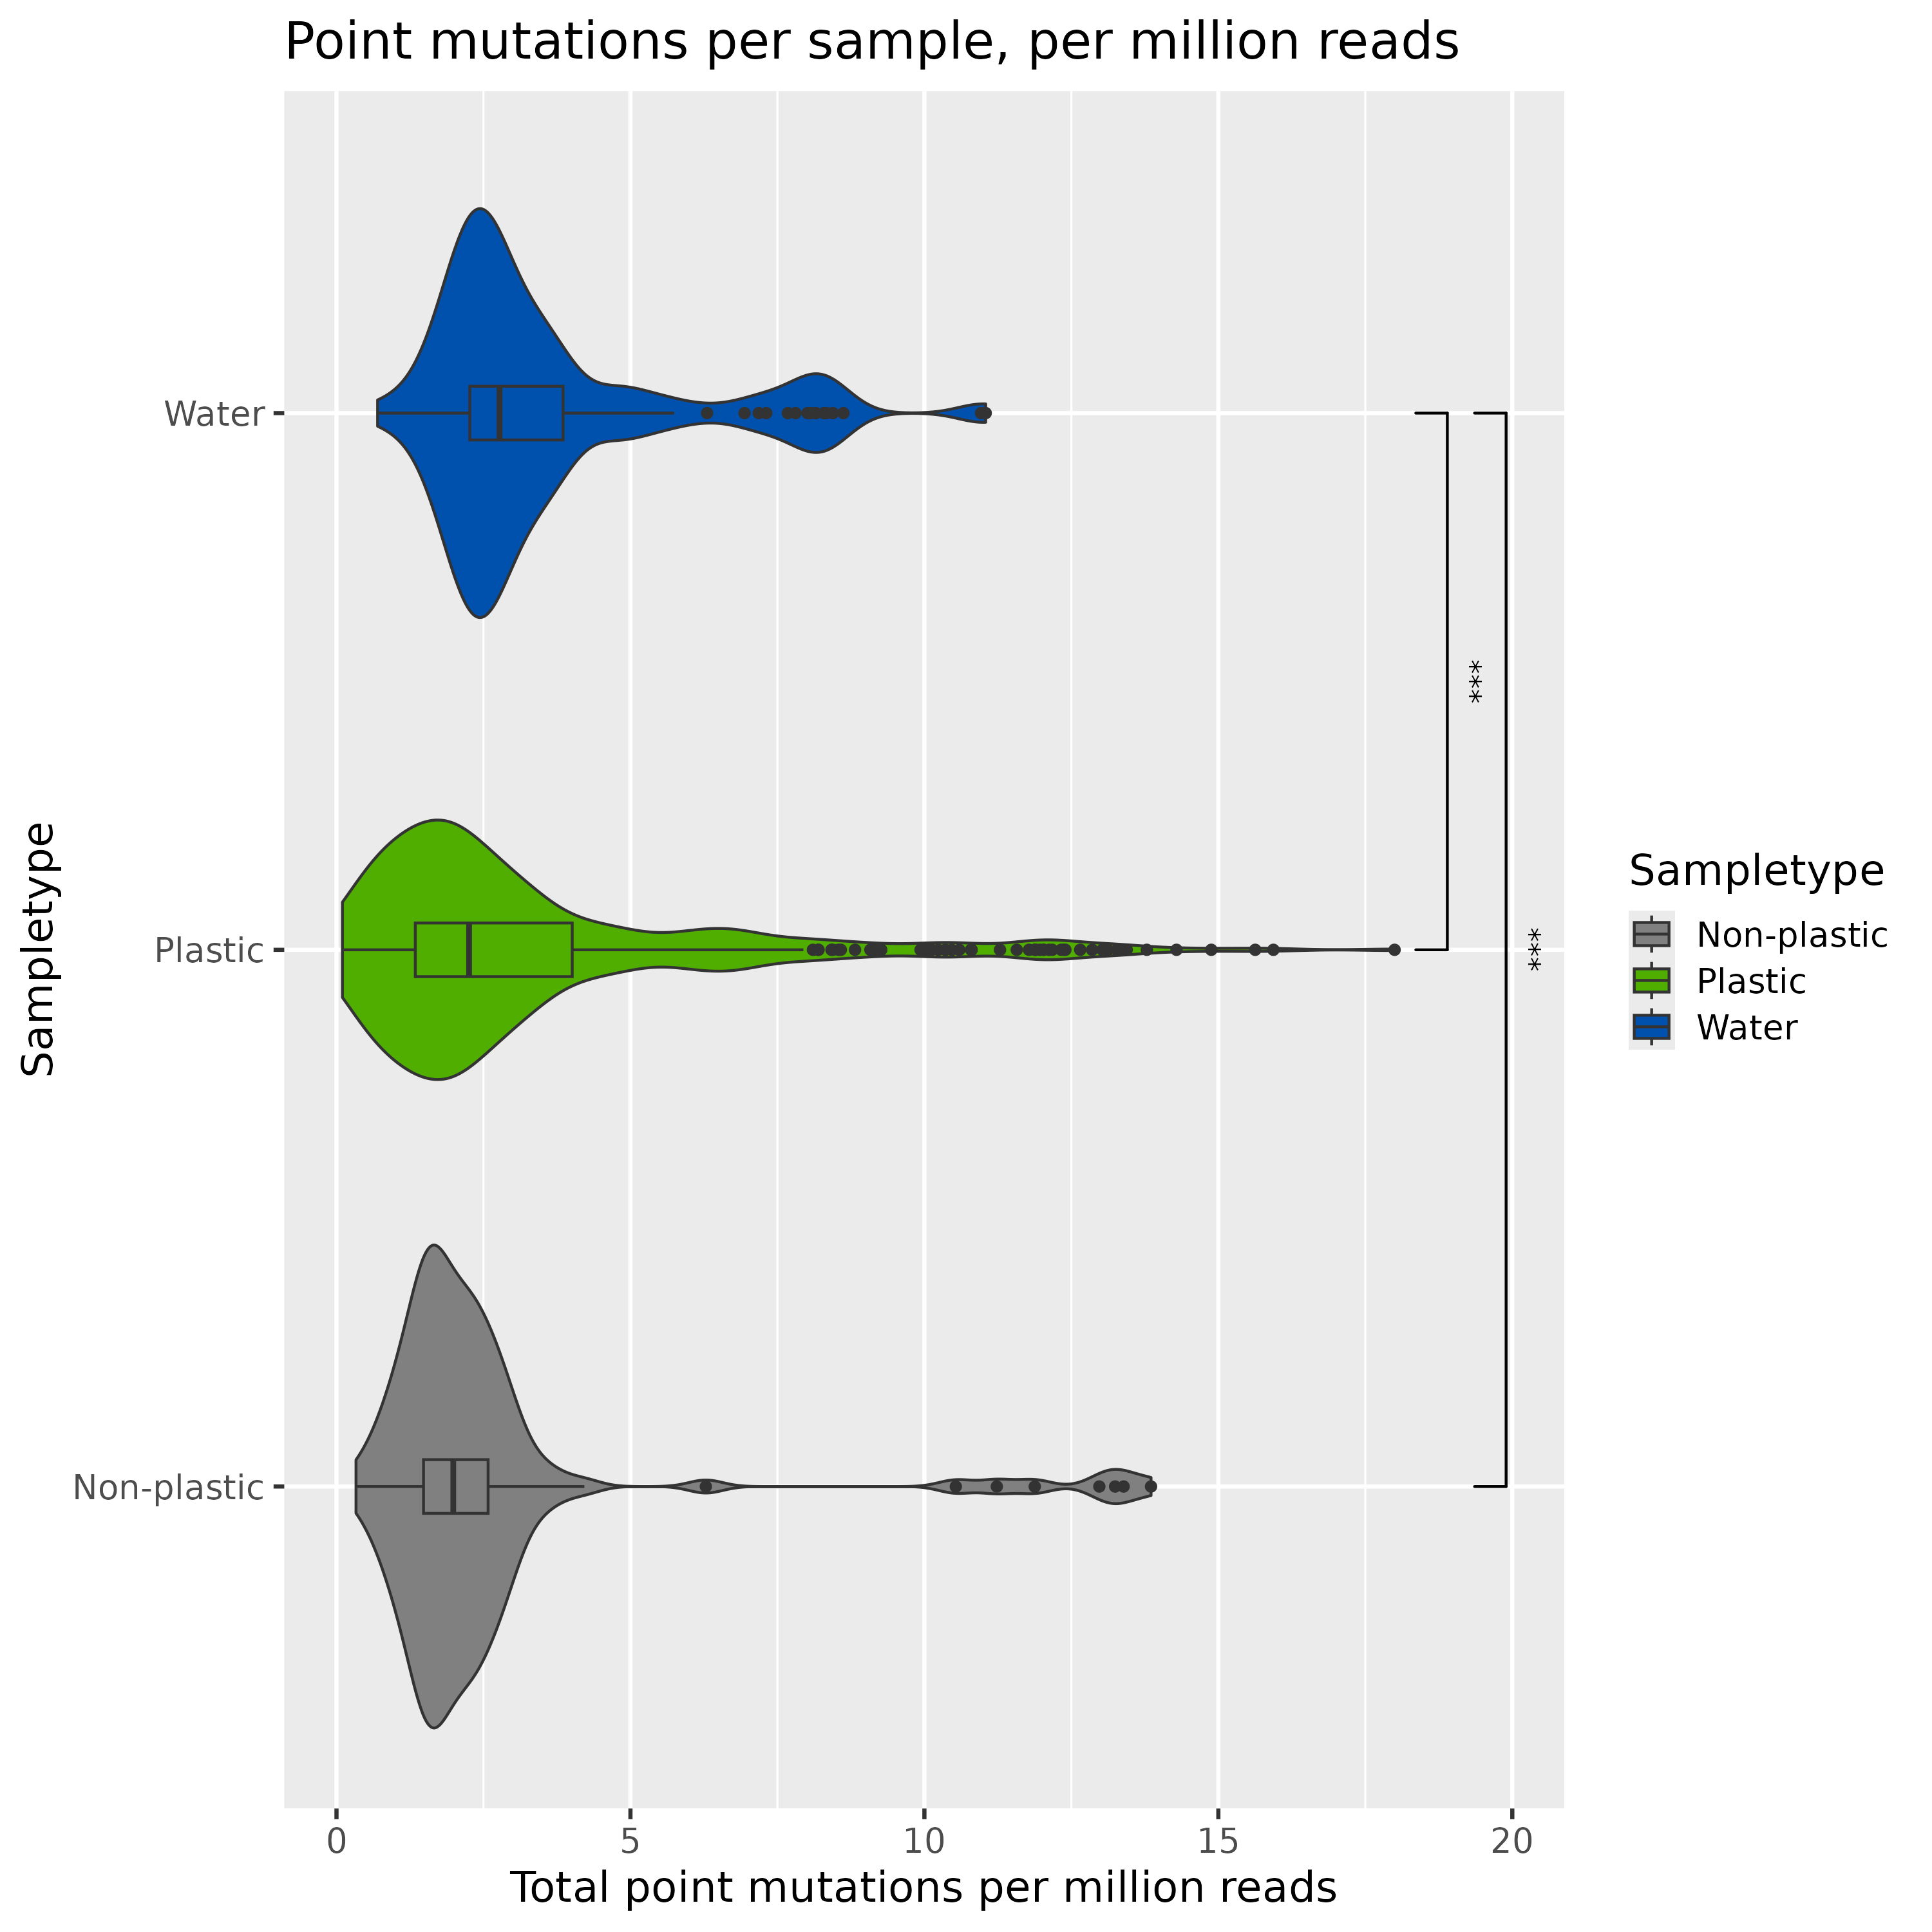
\includegraphics[width = 0.75\textwidth]{figure/hits_per_million_type.png}
    \caption{Total number of mutations per sample, grouped by sampletype. *** = p < 0.001}
    \label{hits_type}
\end{figure}

%There are also differences when comparing between different substrate types in the same way, as shown in figure \ref{hits_substrate}. The significance of these comparisons are shown in \ref{wilcox_hits_substrate}.
There are differences between the total number of point mutations for different substrate types when the total point mutations are compared, as shown in figure \ref{hits_substrate}, where the significance of these comparisons are shown in \ref{wilcox_hits_substrate}.
The plastic substrates PE-fiber-PE (PFP), Ecovio, and BI-OPL show an increase (p < 0.05) in the number of point mutations compared to most other substrates. Both Ecovio and BI-OPL are biodegradable plastics, while PFP is not.
High-density polyethylene (HDPE) show a significant (p < 0.05) decrease in the number of point mutations compared to all other substrates.
%The result of grouping the samples by substrate type instead is shown in figure \ref{hits_substrate}, which show that there was a great difference in total hit count per million between different substrate types. 
%Figure \ref{wilcox_hits_substrate} show the statistical significance of the comparison, where a wilcoxon test was done for the Substrate versus the Reference. The figure also shows the sign of the pseudo-mean for the comparison, labelled "Change", and is set to Increase if the pseudo-mean is positive and Decrease if it negative.
%Note that all comparisons were done, but only the significant ones (p < 0.05) are shown.
%There are some plastic substrates which increased comp ared to most other substrates. These include PFP, Ecovio and BI-OPL. 
The plastic substrates which show a significant increase compared to any of the water substrates are polyhydroxybutyrate (PHB), PE-fiber (PF), polybutylene adipate terephthalate (PBAT), low-density polyethylene (LDPE), Ecovio, and BI-OPL.
The soil substrate also show an overall increase in point-mutation rates compared to most other substrates, as does freshwater and seawater, with the exception of PFP, Ecovio, and BI-OPL. 

% Based on the result in these figures, it is evident that the number of point mutations which confer antibiotic resistance are not more prevalent on all plastics, but instead that specific plastic substrates increase this count.
% These substrates include PFP, Ecovio, and BI-OPL. The latter two are biodegradable plastics which contain a blend of PBAT and PLA. 


\begin{figure}[h!]
    \centering
    \subfloat[\label{hits_substrate}]{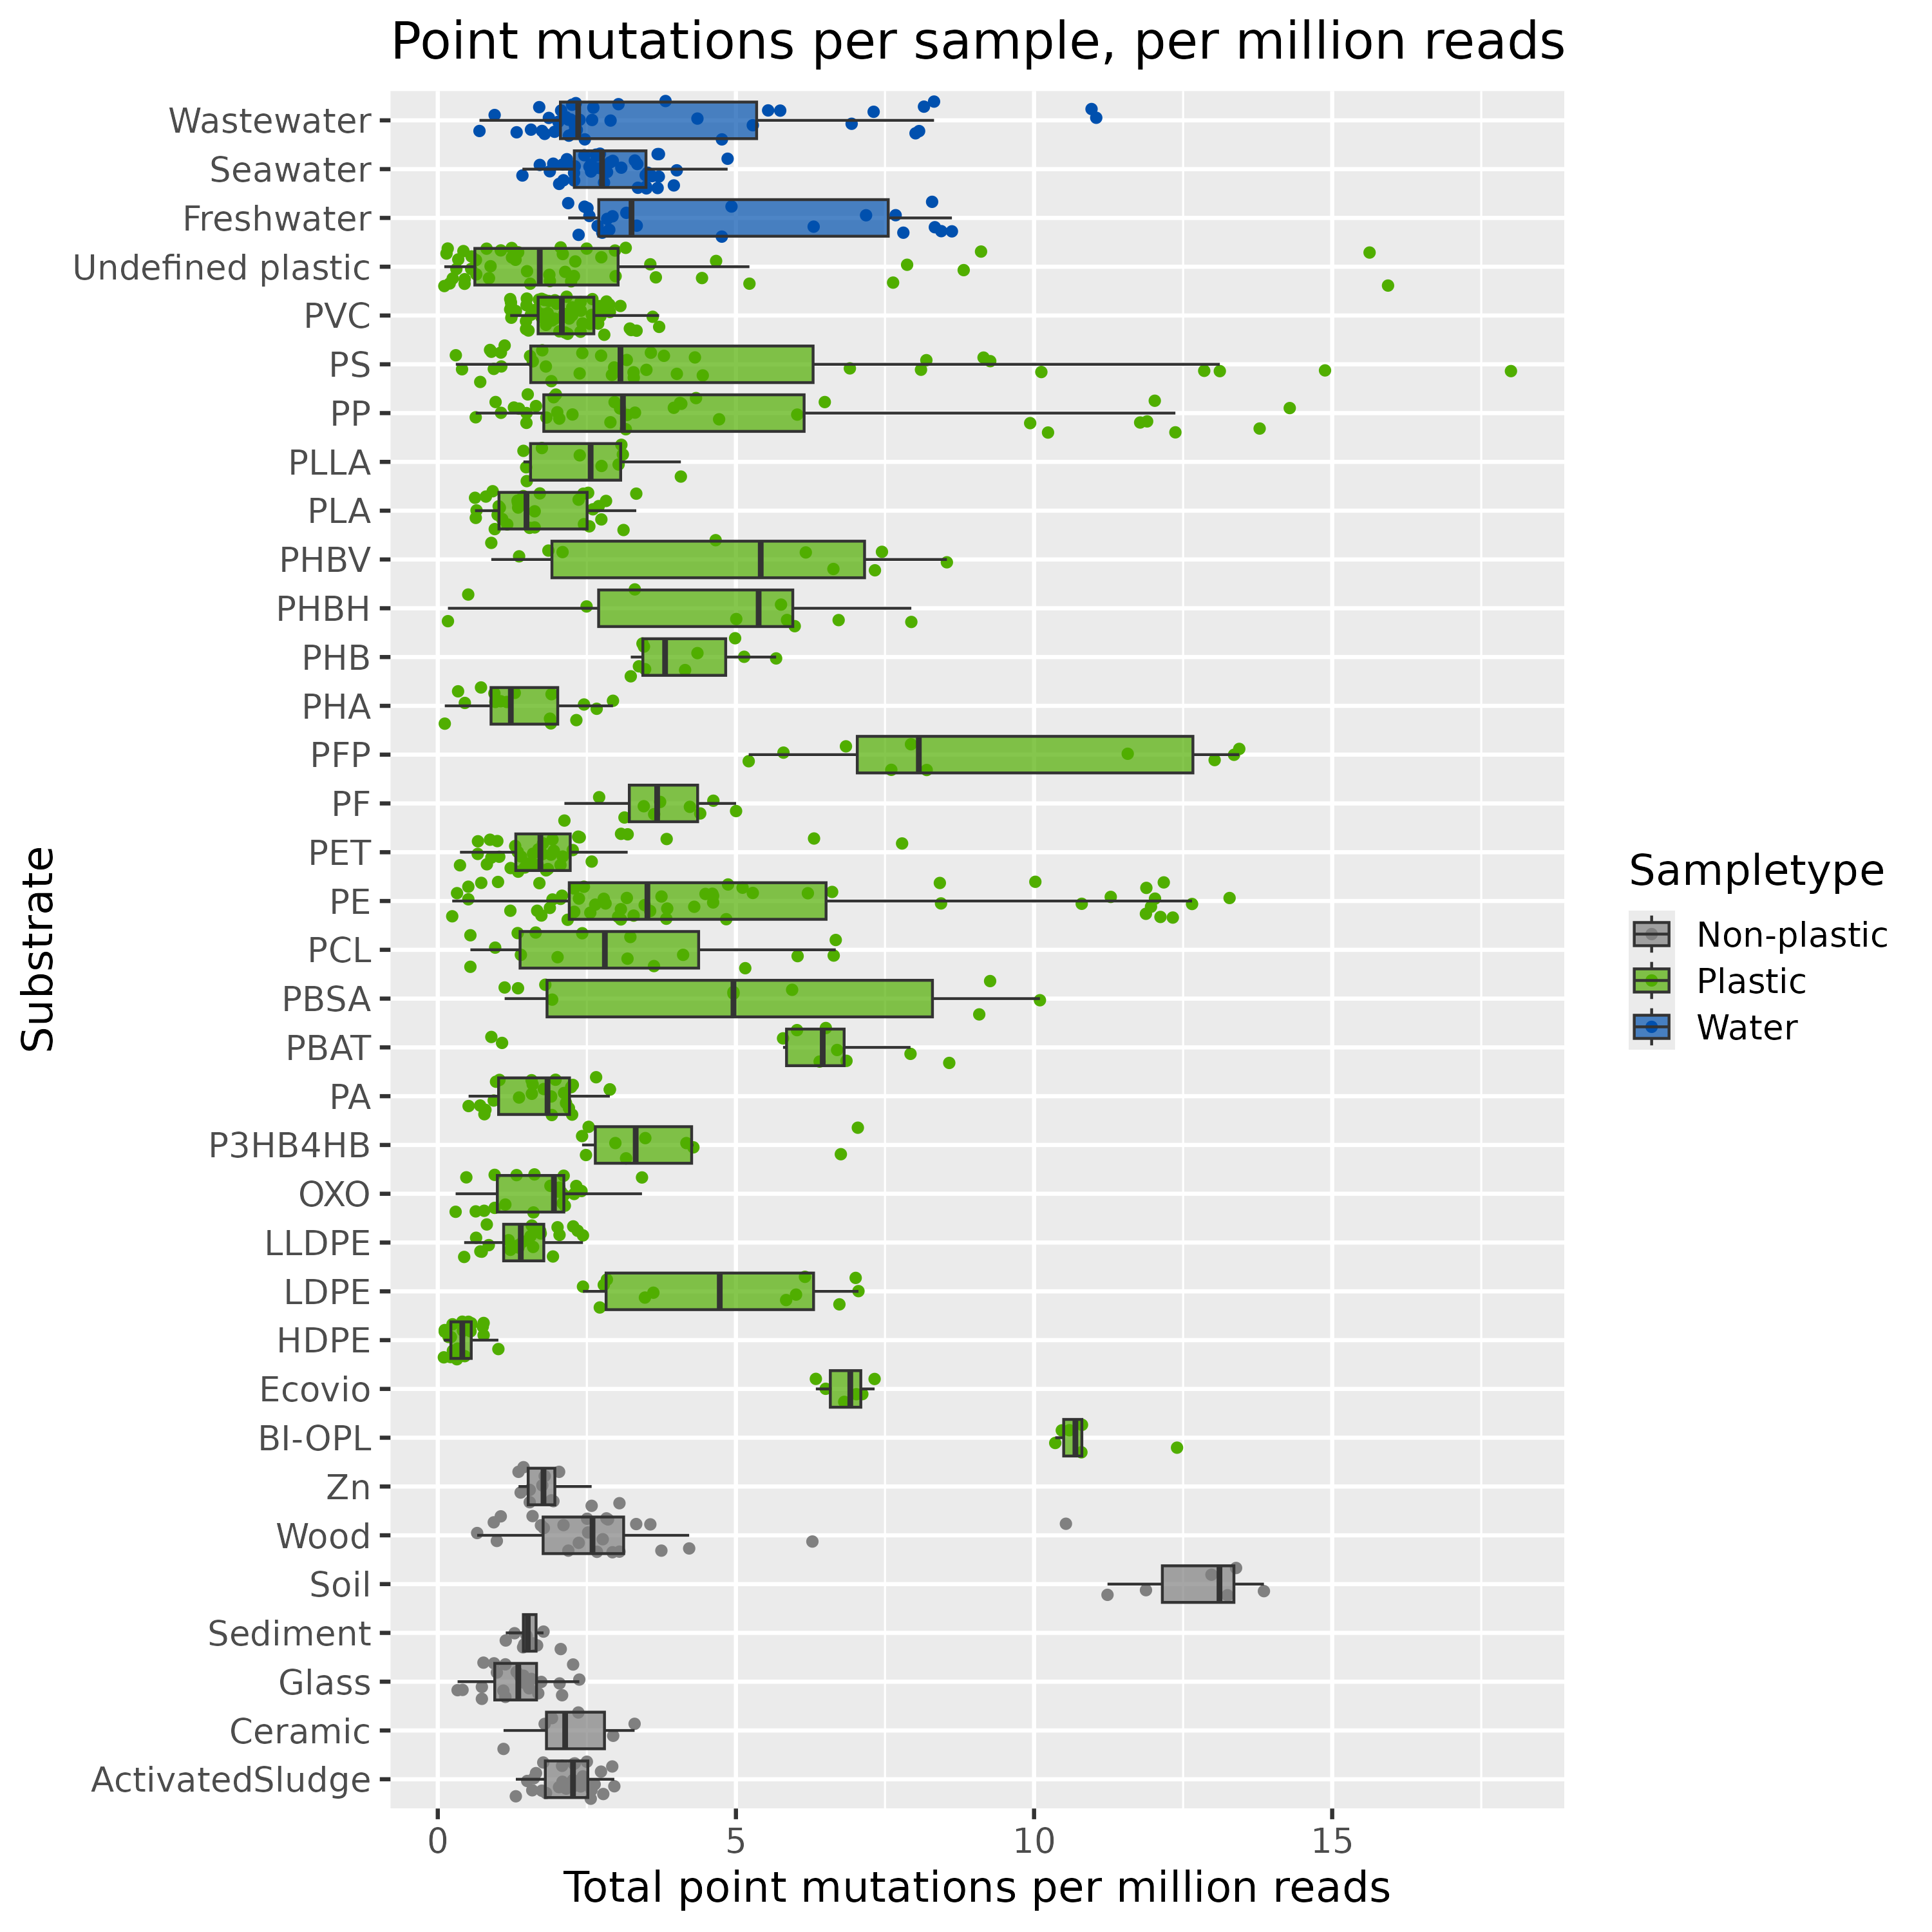
\includegraphics[width=0.5\textwidth]{figure/hits_per_million_substrate.png}}
    \subfloat[\label{wilcox_hits_substrate}]{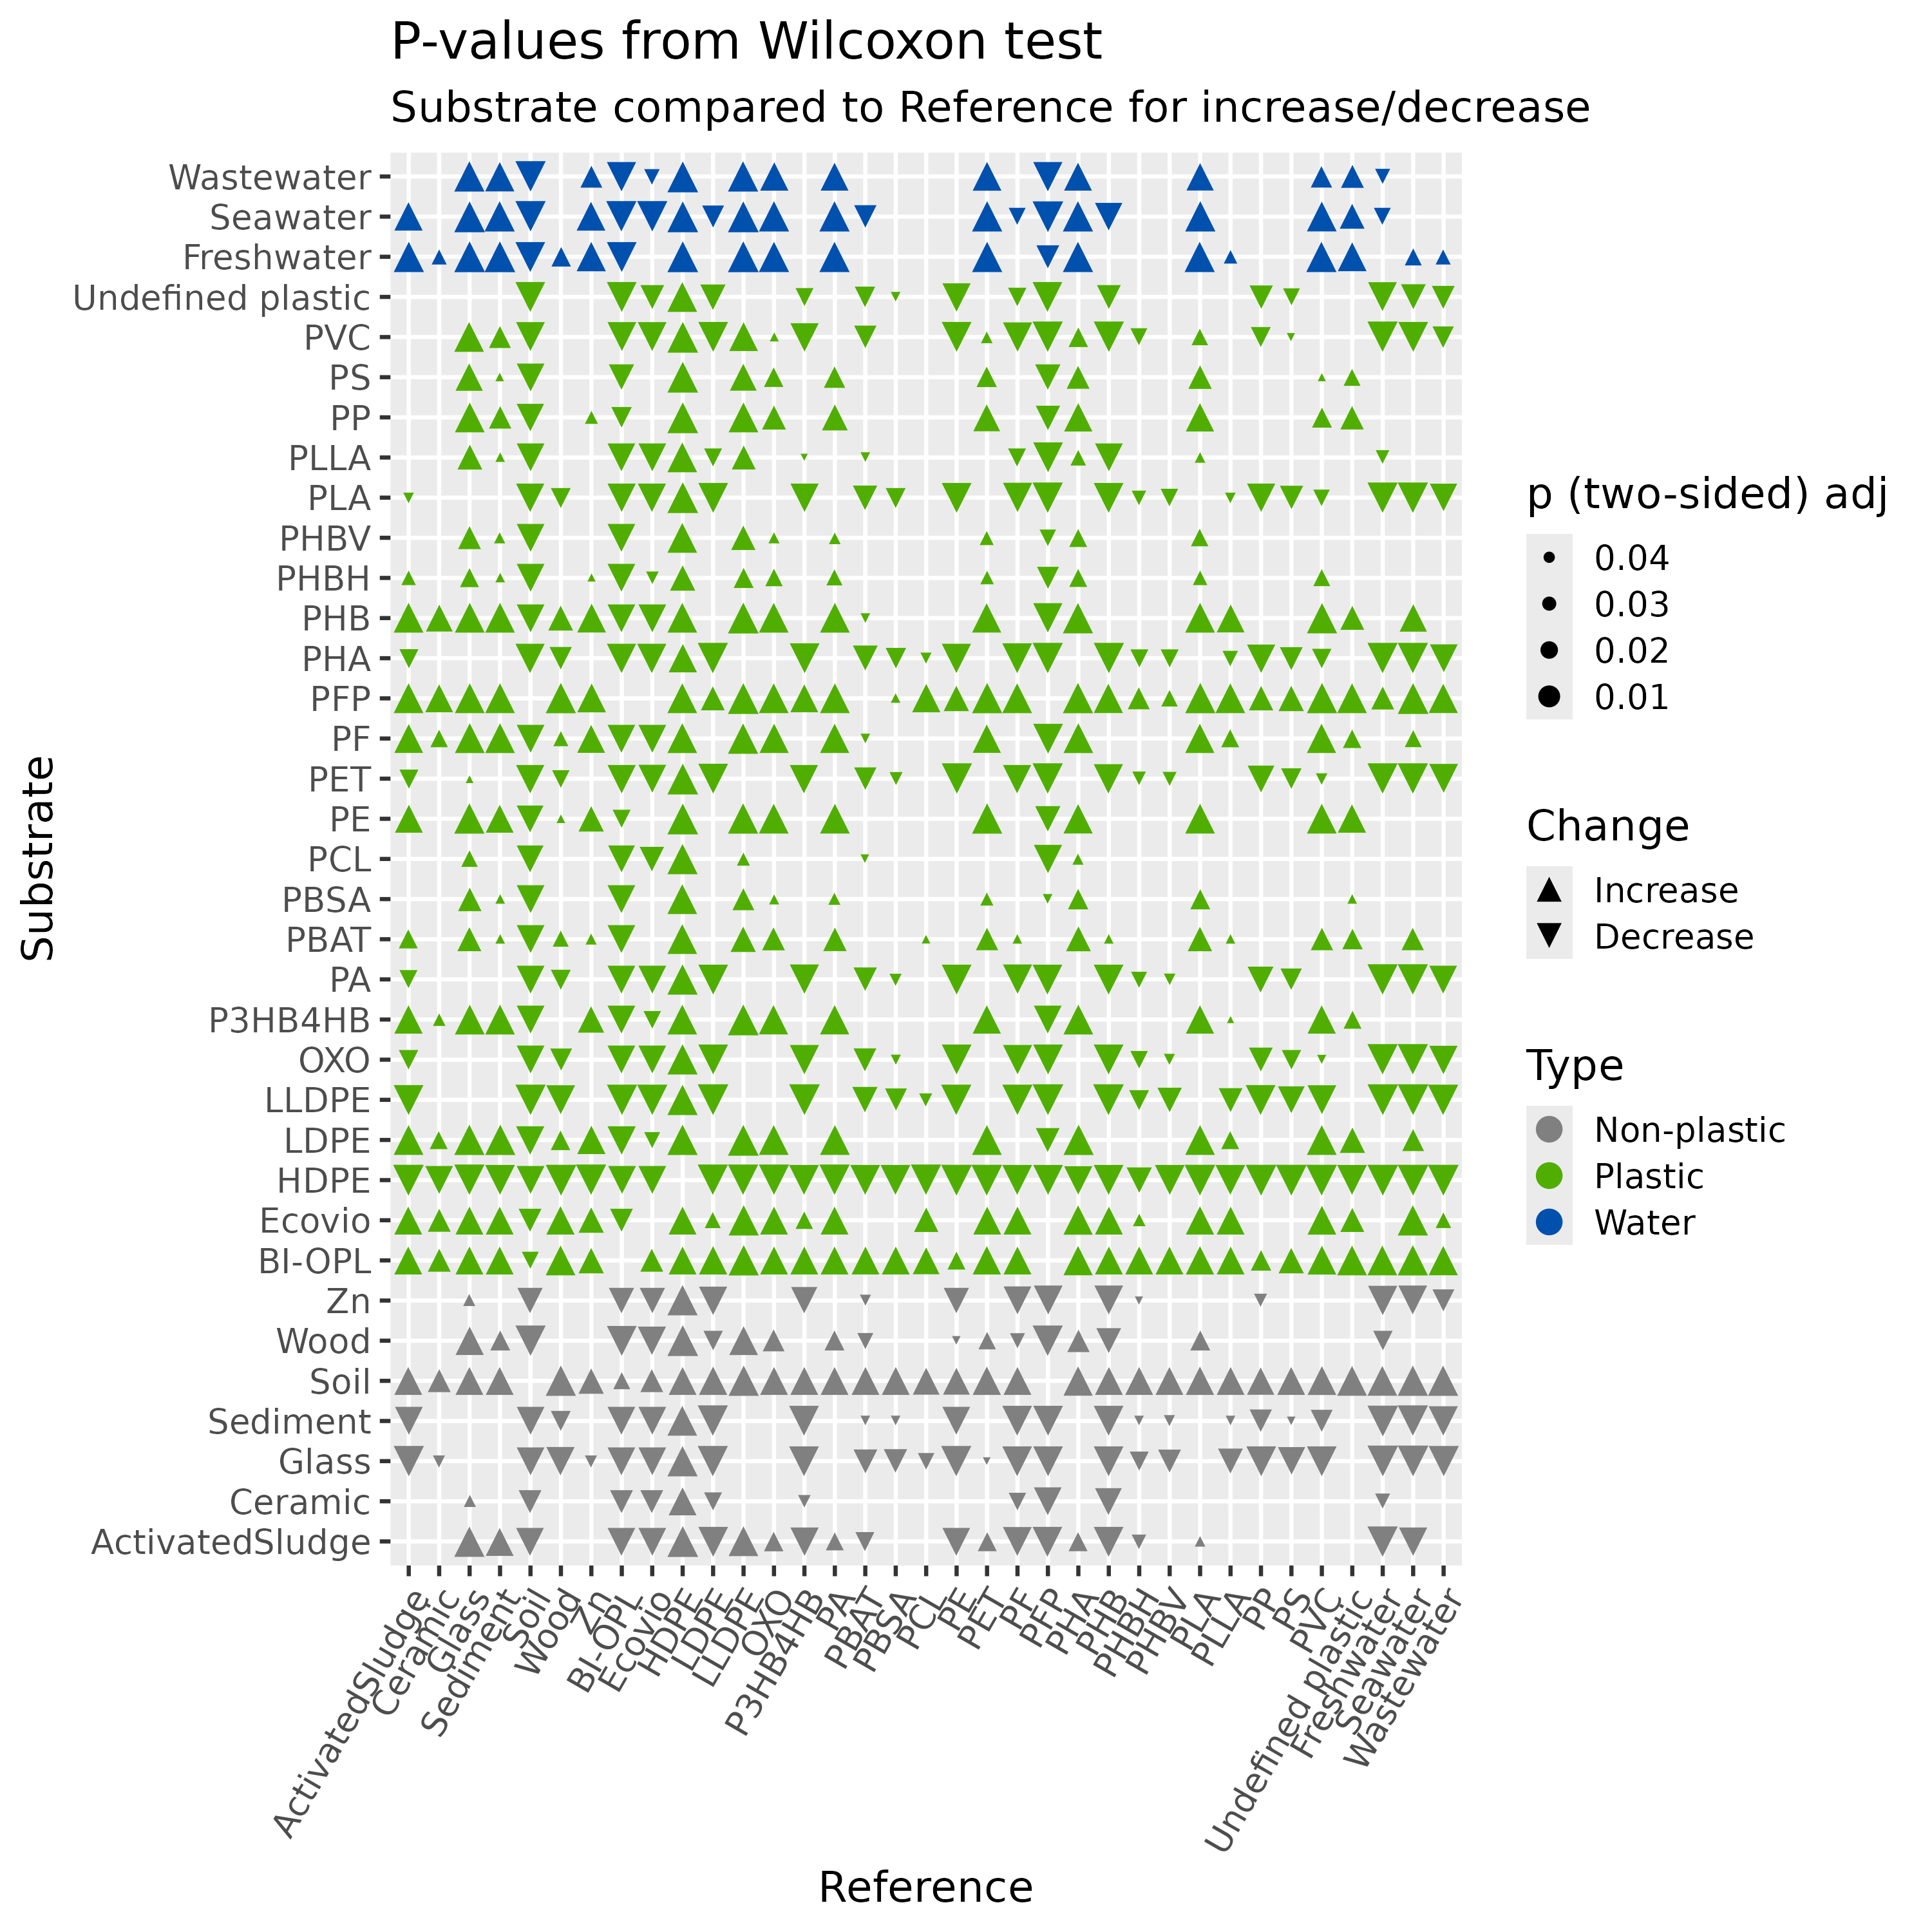
\includegraphics[width=0.5\textwidth]{figure/wilcox_hits_substrates.png}}
    \caption{(a) Point mutations per million reads. (b) p-values from Wilcoxon test for the number of point mutations of Subtrate versus Reference}
    \label{both_hits_substrate}
\end{figure}


\section{Mean mutation percentage}
%todo{Mention how the samples are collected, that they take the biofilm and sequence that? Check in a study what they do}
The following section present the results of using the mean mutation percentage instead of the total number of point mutations, which has the advantage of reducing the impact of genes which a large number of reads map to, instead using the relative mutation frequency of each individual gene.
As described above this mean value can be calculated for either the samples or the mutations. These values tell you different things, where in the first case it estimates how mutated the genes are in the samples, i.e. "this sample has a mean mutation percentage of 3\%".
In the latter case it estimates how mutated specific genes are in the different substrates, i.e. "mutation A has a mean mutation percentage of 25\% in freshwater" \todo{Same problem as in Method, how to describe it.}.
% The advantage of this approach is that the relative mutation frequency of the gene is used instead of the total number of point mutations, which normalizes the mutation rate and reduces the impact of genes which a large number of reads map to.

%\subsection{Mean mutation percentage of samples} 
%\subsubsection{Alternative 1, combined plots, otherwise two separate larger plots, see \ref{mean_samples_substrate_full} and \ref{wilcox_samples_substrates_full}}
%The mean mutation percentage was calculated for every sample, and 
Figure \ref{mean_samples_sampletype} show the mean mutation percent grouped by the type of sample.
There is a significant difference (Wilcoxon test: p < 0.001) between the water group and the plastic group, where the plastic group has a lower mean mutation percentage in comparison to the water group. None of the other groups displayed any significant difference (p < 0.05) between them.

%\todo{Remove n.s.?}
\begin{figure}[h!]
    \centering
    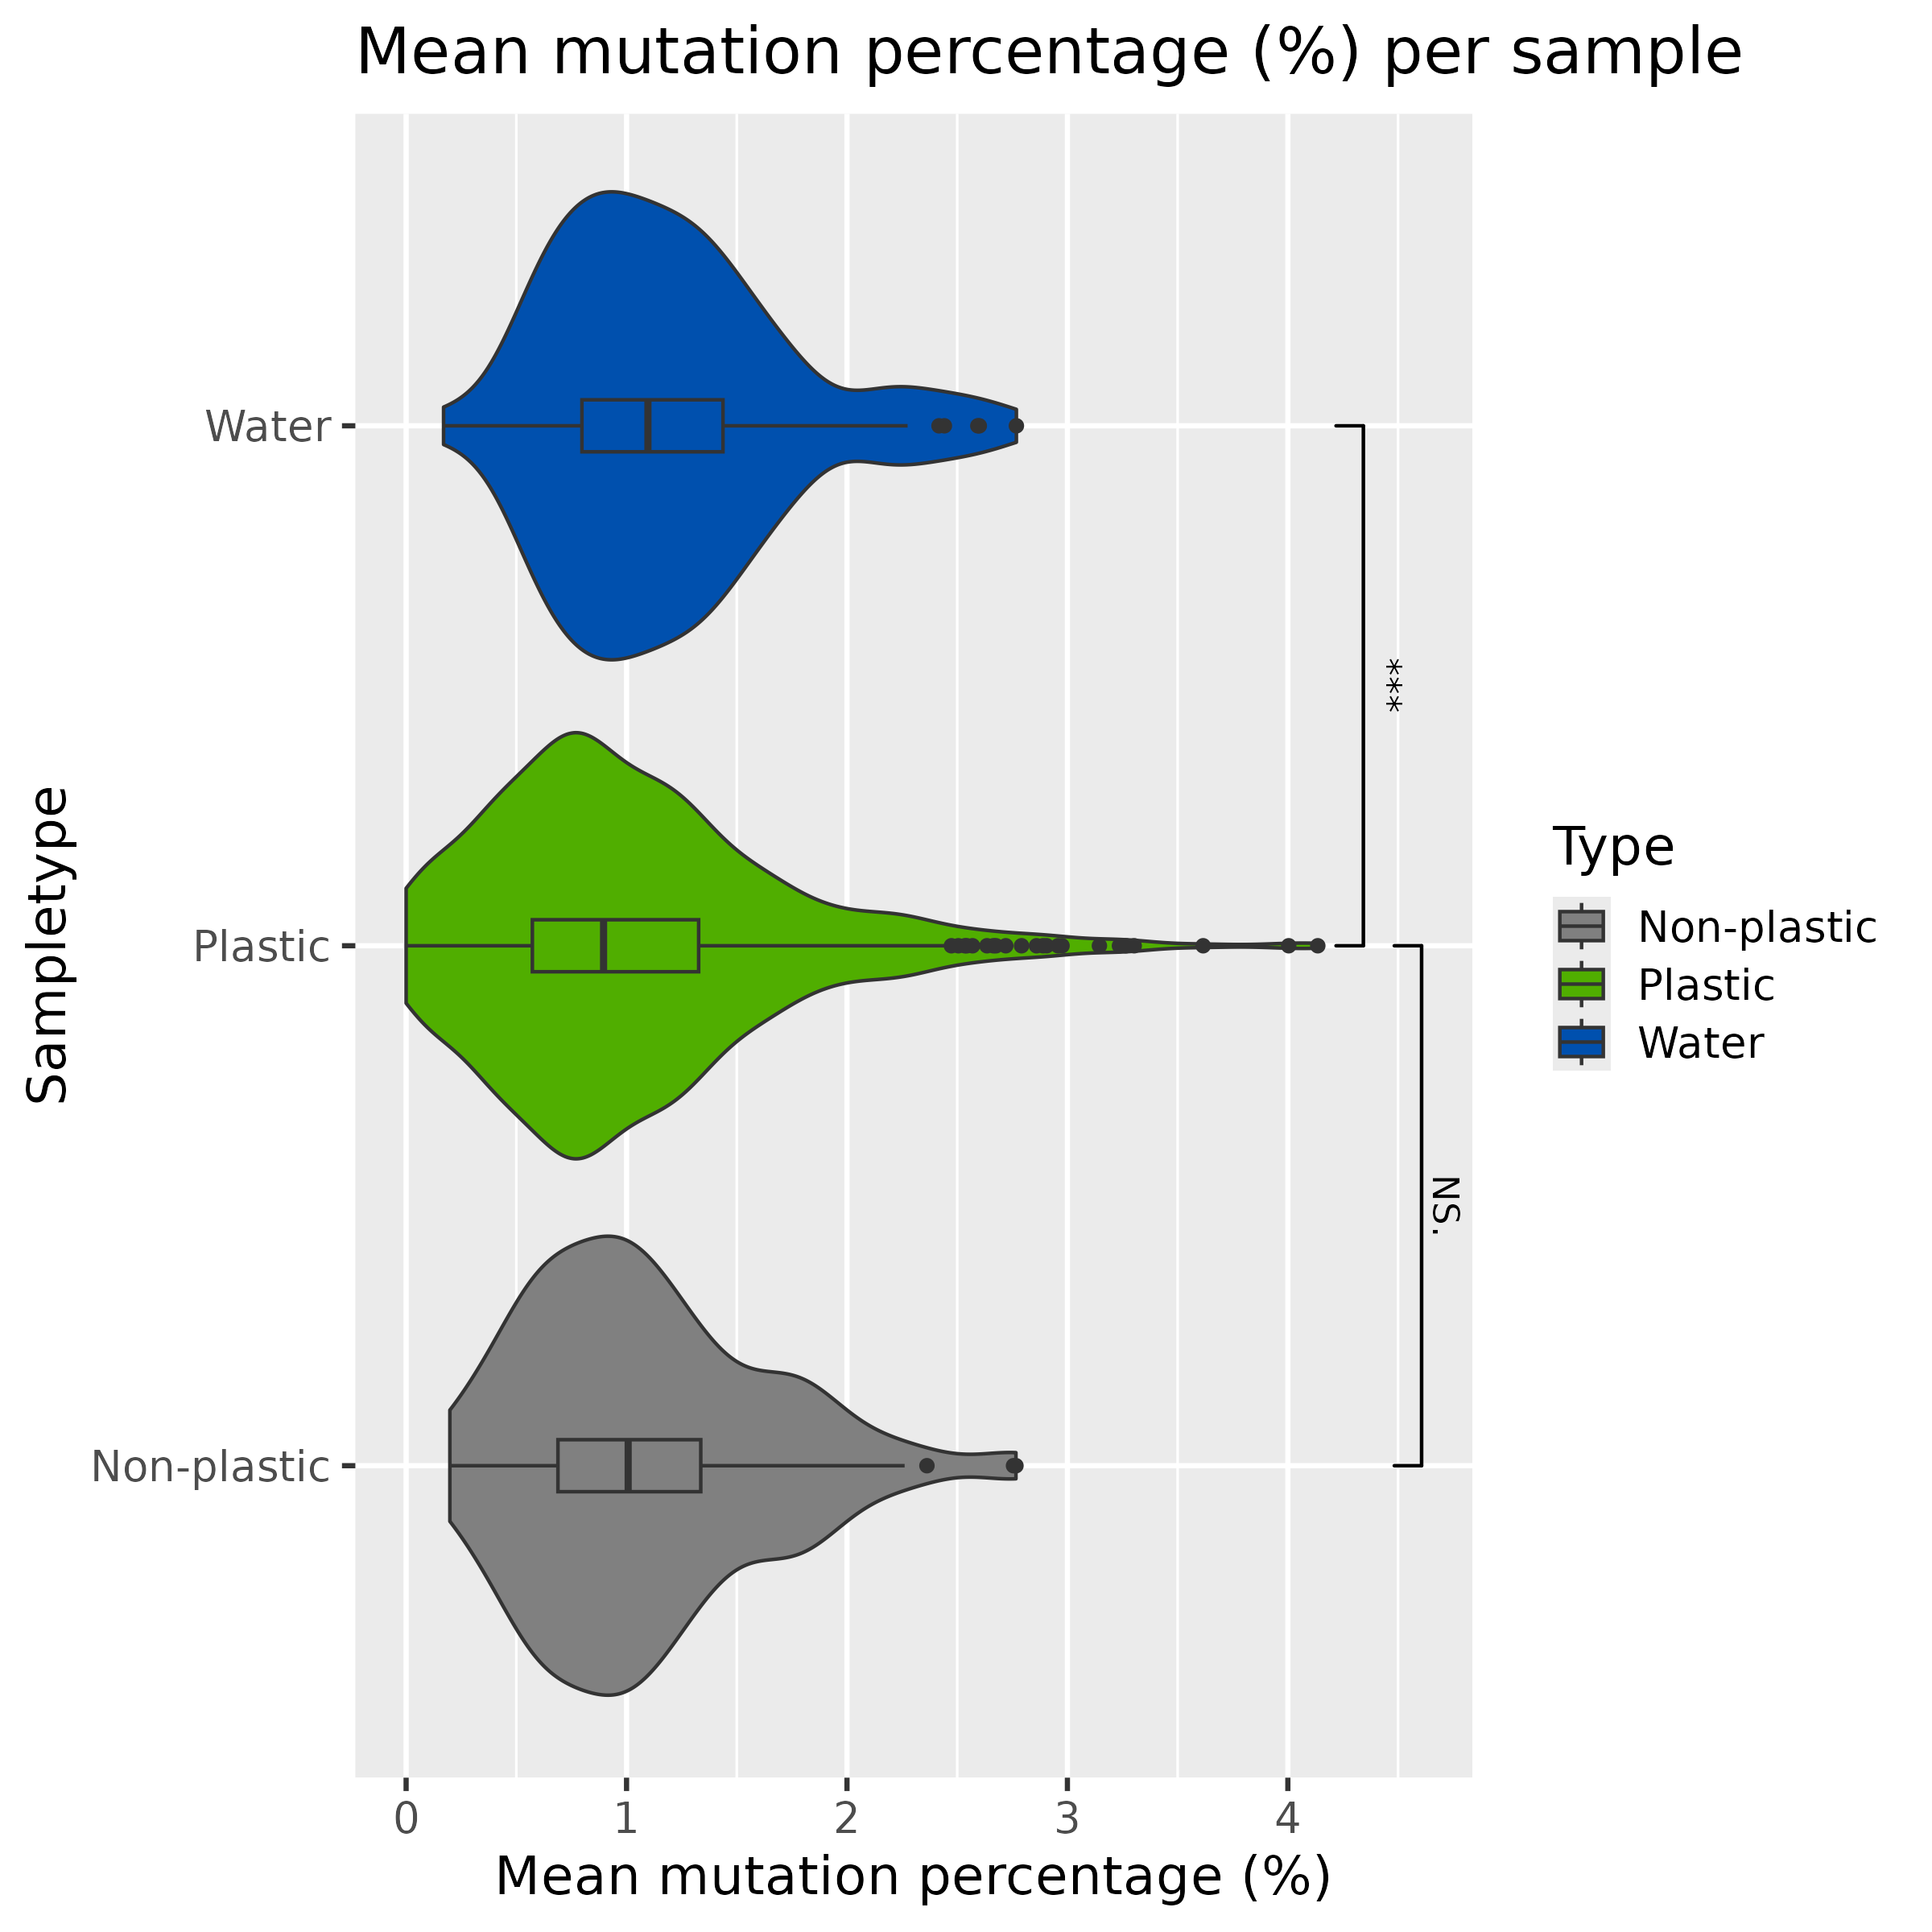
\includegraphics[width = 0.6\textwidth]{figure/mean_samples_sampletype.png}
    \caption{Mean mutation percentage (\%) per sample, grouped by sampletype. * = p < 0.05, *** = p < 0.001}
    \label{mean_samples_sampletype}
\end{figure}
%\todo{P-values-table in appendix or not at all?)}

% \begin{table}[h]
% \caption{p-values from Wilcoxon test between sampletypes}
% \label{wilcox_samples_sampletype}
% \begin{tabular}{@{}llllll@{}}
% \toprule
% Sampletype A & Sampletype B & Significance & Change   & p (two-sided) & pseudo\_mean  \\ \midrule
% Non-plastic  & Plastic      & *            & Increase & 0.0473  &  0.0012  \\
% Water        & Plastic      & ***          & Increase & 0.0005  &  0.0020  \\
% Non-plastic  & Water        & ns           & Decrease & 0.1801  & -0.0009 \\
% Plastic      & Water        & ***          & Decrease & 0.0005  & -0.0020 \\
% Plastic      & Non-plastic  & *            & Decrease & 0.0473  & -0.0012 \\
% Water        & Non-plastic  & ns           & Increase & 0.1801  &  0.0009 \\ \bottomrule
% \end{tabular}
% \end{table}


In figure \ref{mean_samples_substrate} the samples are instead grouped by substrate type, which shows that there are differences for different plastics, as well as other substrates.
Figure \ref{wilcox_samples_substrate} show the statistical significance of the comparison, when a Wilcoxon test was done for the Substrate versus the Reference, as well as if there is an increase of the pseudo-mean compared to the reference.
Note that all comparisons were done, but only the significant ones (p < 0.05) are shown.
There are some plastics that has a significant, higher, mean mutation percentage than most other substrates. These include PFP, LDPE, Ecovio and BI-OPL. The last two plastics are biodegradable plastics.
The plastic substrates that has a significant higher mean mutation percentage than seawater or wastewater include polyvinyl chloride (PVC) and PF in addition to PFP, LDPE, Ecovio and BI-OPL.
There are also some plastics which have significantly different lower mean mutation percentage than almost all other substrates, the most notable of which is high-density polyethylene (HDPE), poly(3-hydroxybutyrate-co-3-hydroxyvalerate) (PHBV) and polyhydroxyalkanoate (PHA), of which the latter two are biodegradable polymers while the first one is not.
Almost all substrates have a significantly different lower mean mutation percentage than the freshwater samples and the soil samples, the exception of which is Ecovio, BI-OPL, and PFP where there is no significant (p < 0.05) difference. 
%The soil samples have a significantly higher (p < 0.001) mean mutation percentage compared to most other substrates. 
%todo{meh, "which is expected from previous studies" + ref? Idk varför det nämns}.


\begin{figure}[h!]
    \centering
    \subfloat[\label{mean_samples_substrate}]{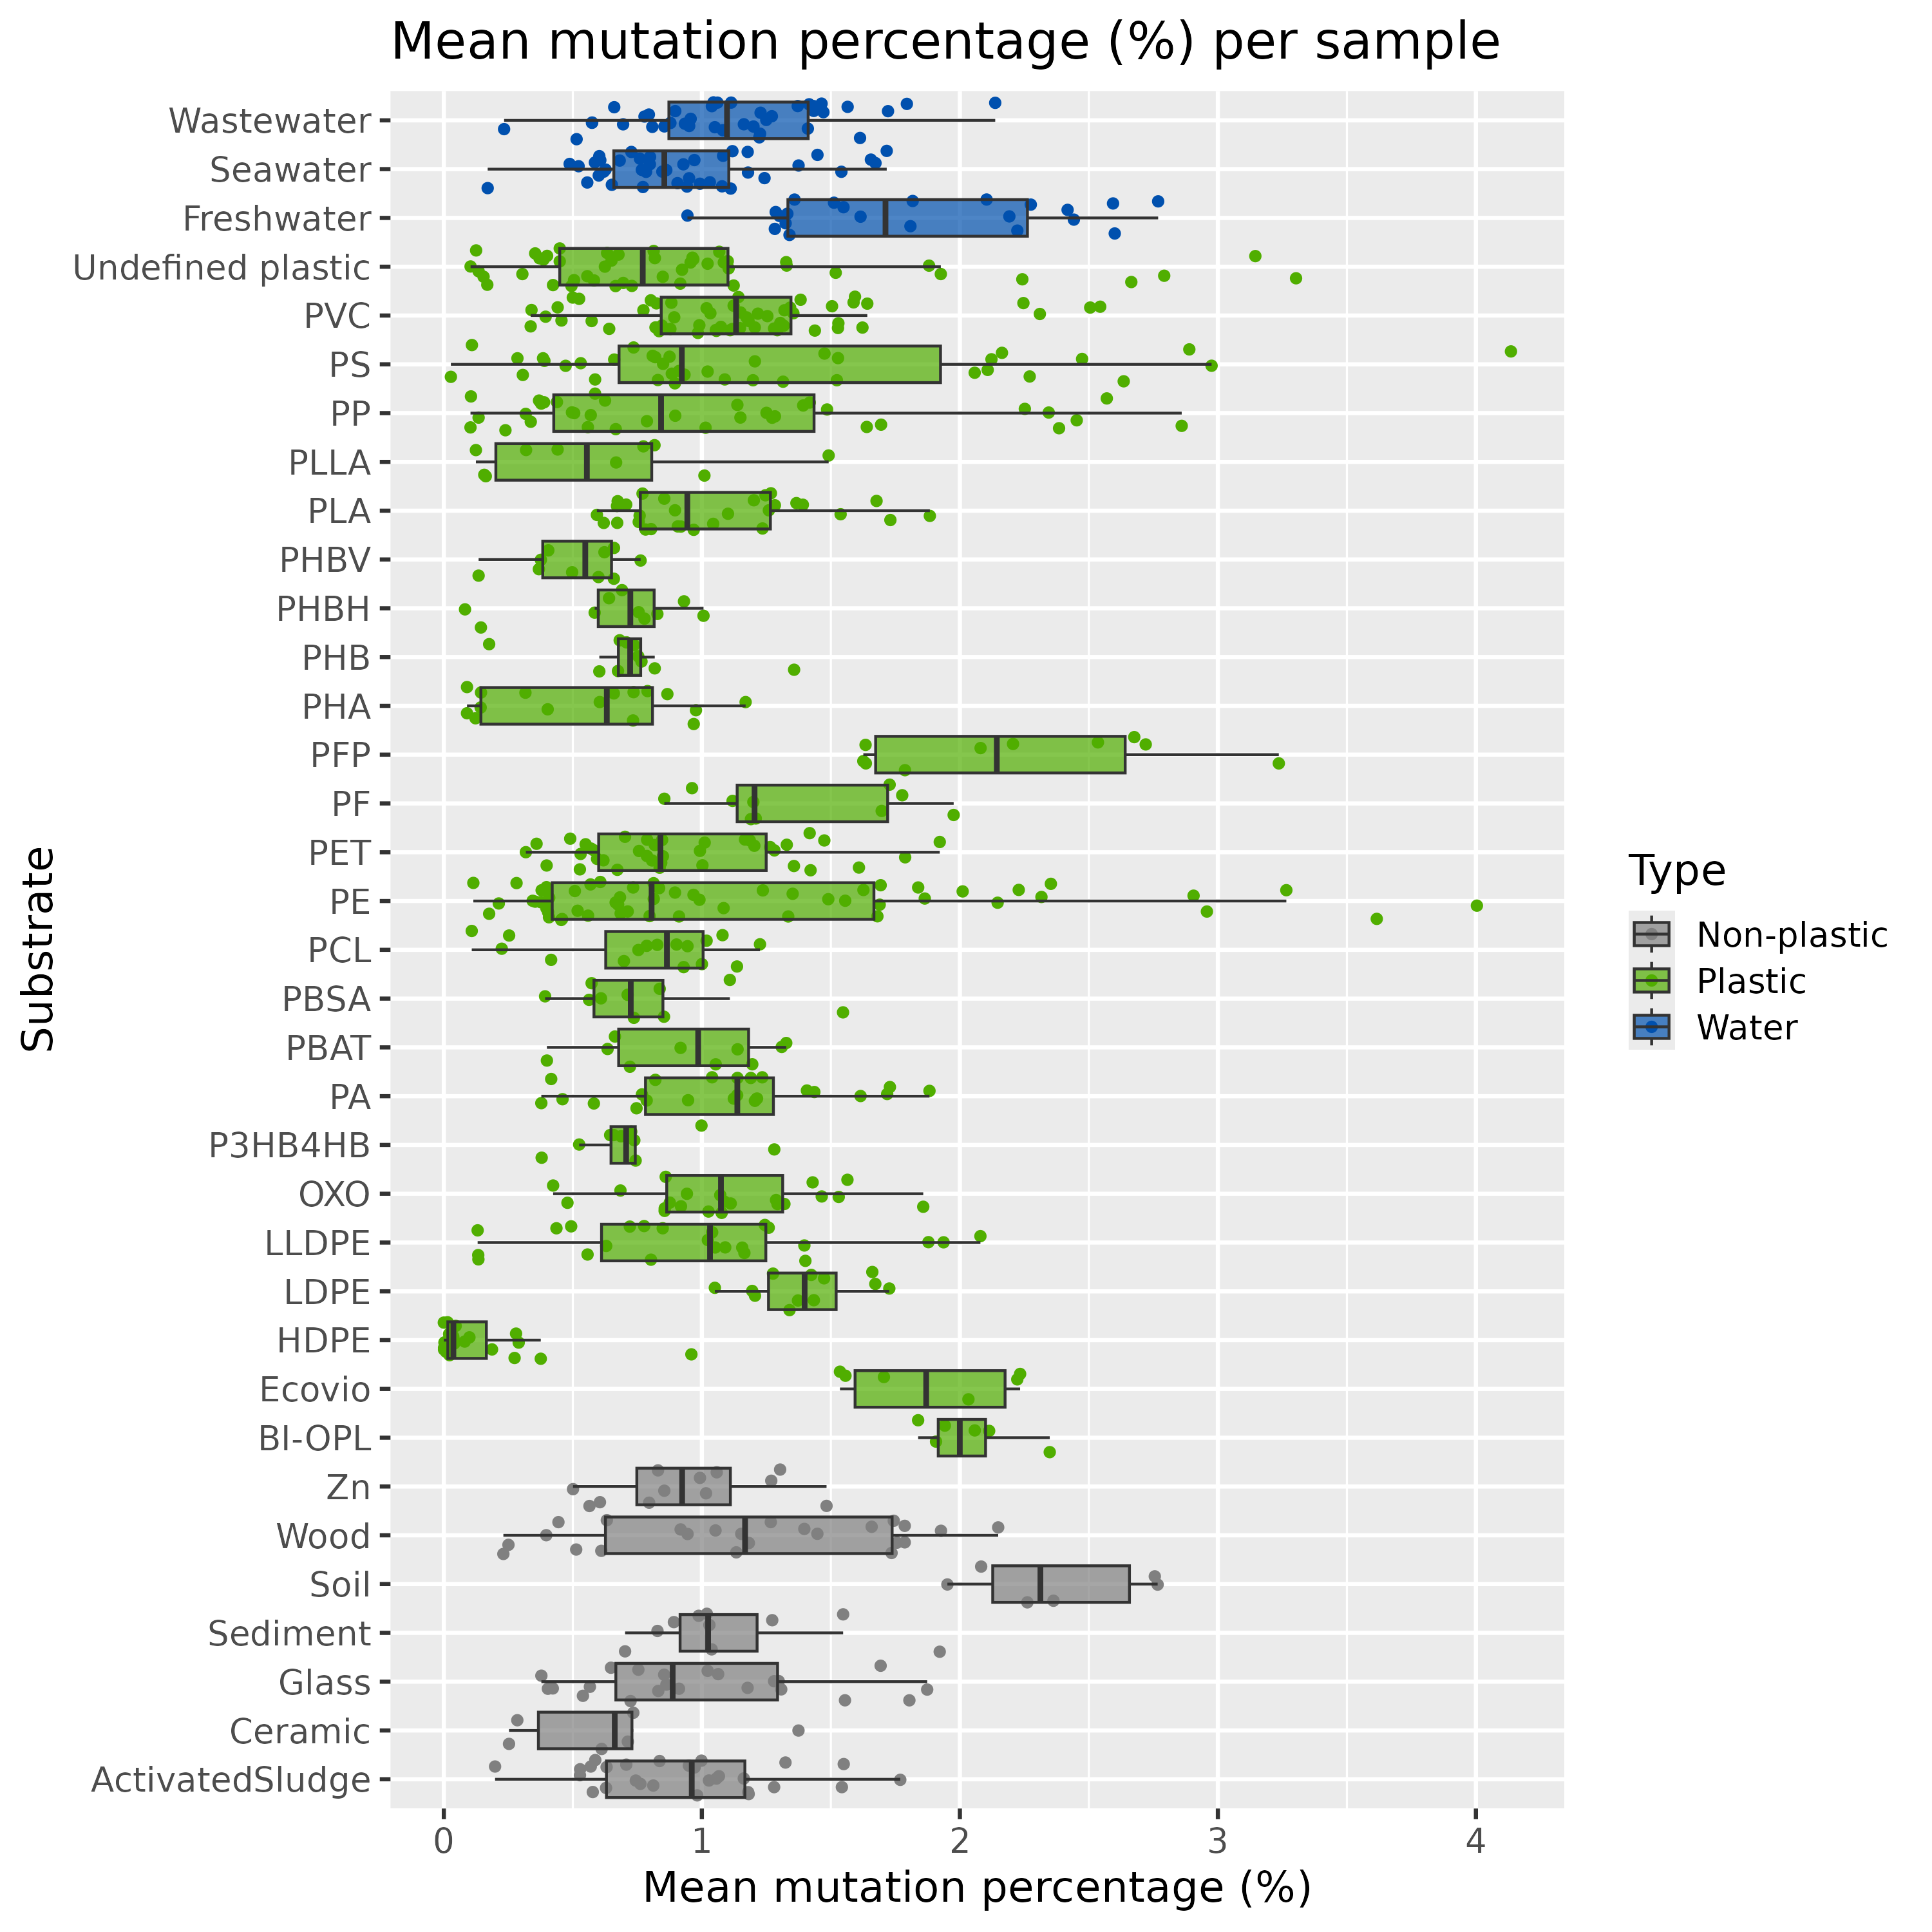
\includegraphics[width=0.5\textwidth]{figure/mean_samples_substrate.png}}
    \subfloat[\label{wilcox_samples_substrate}]{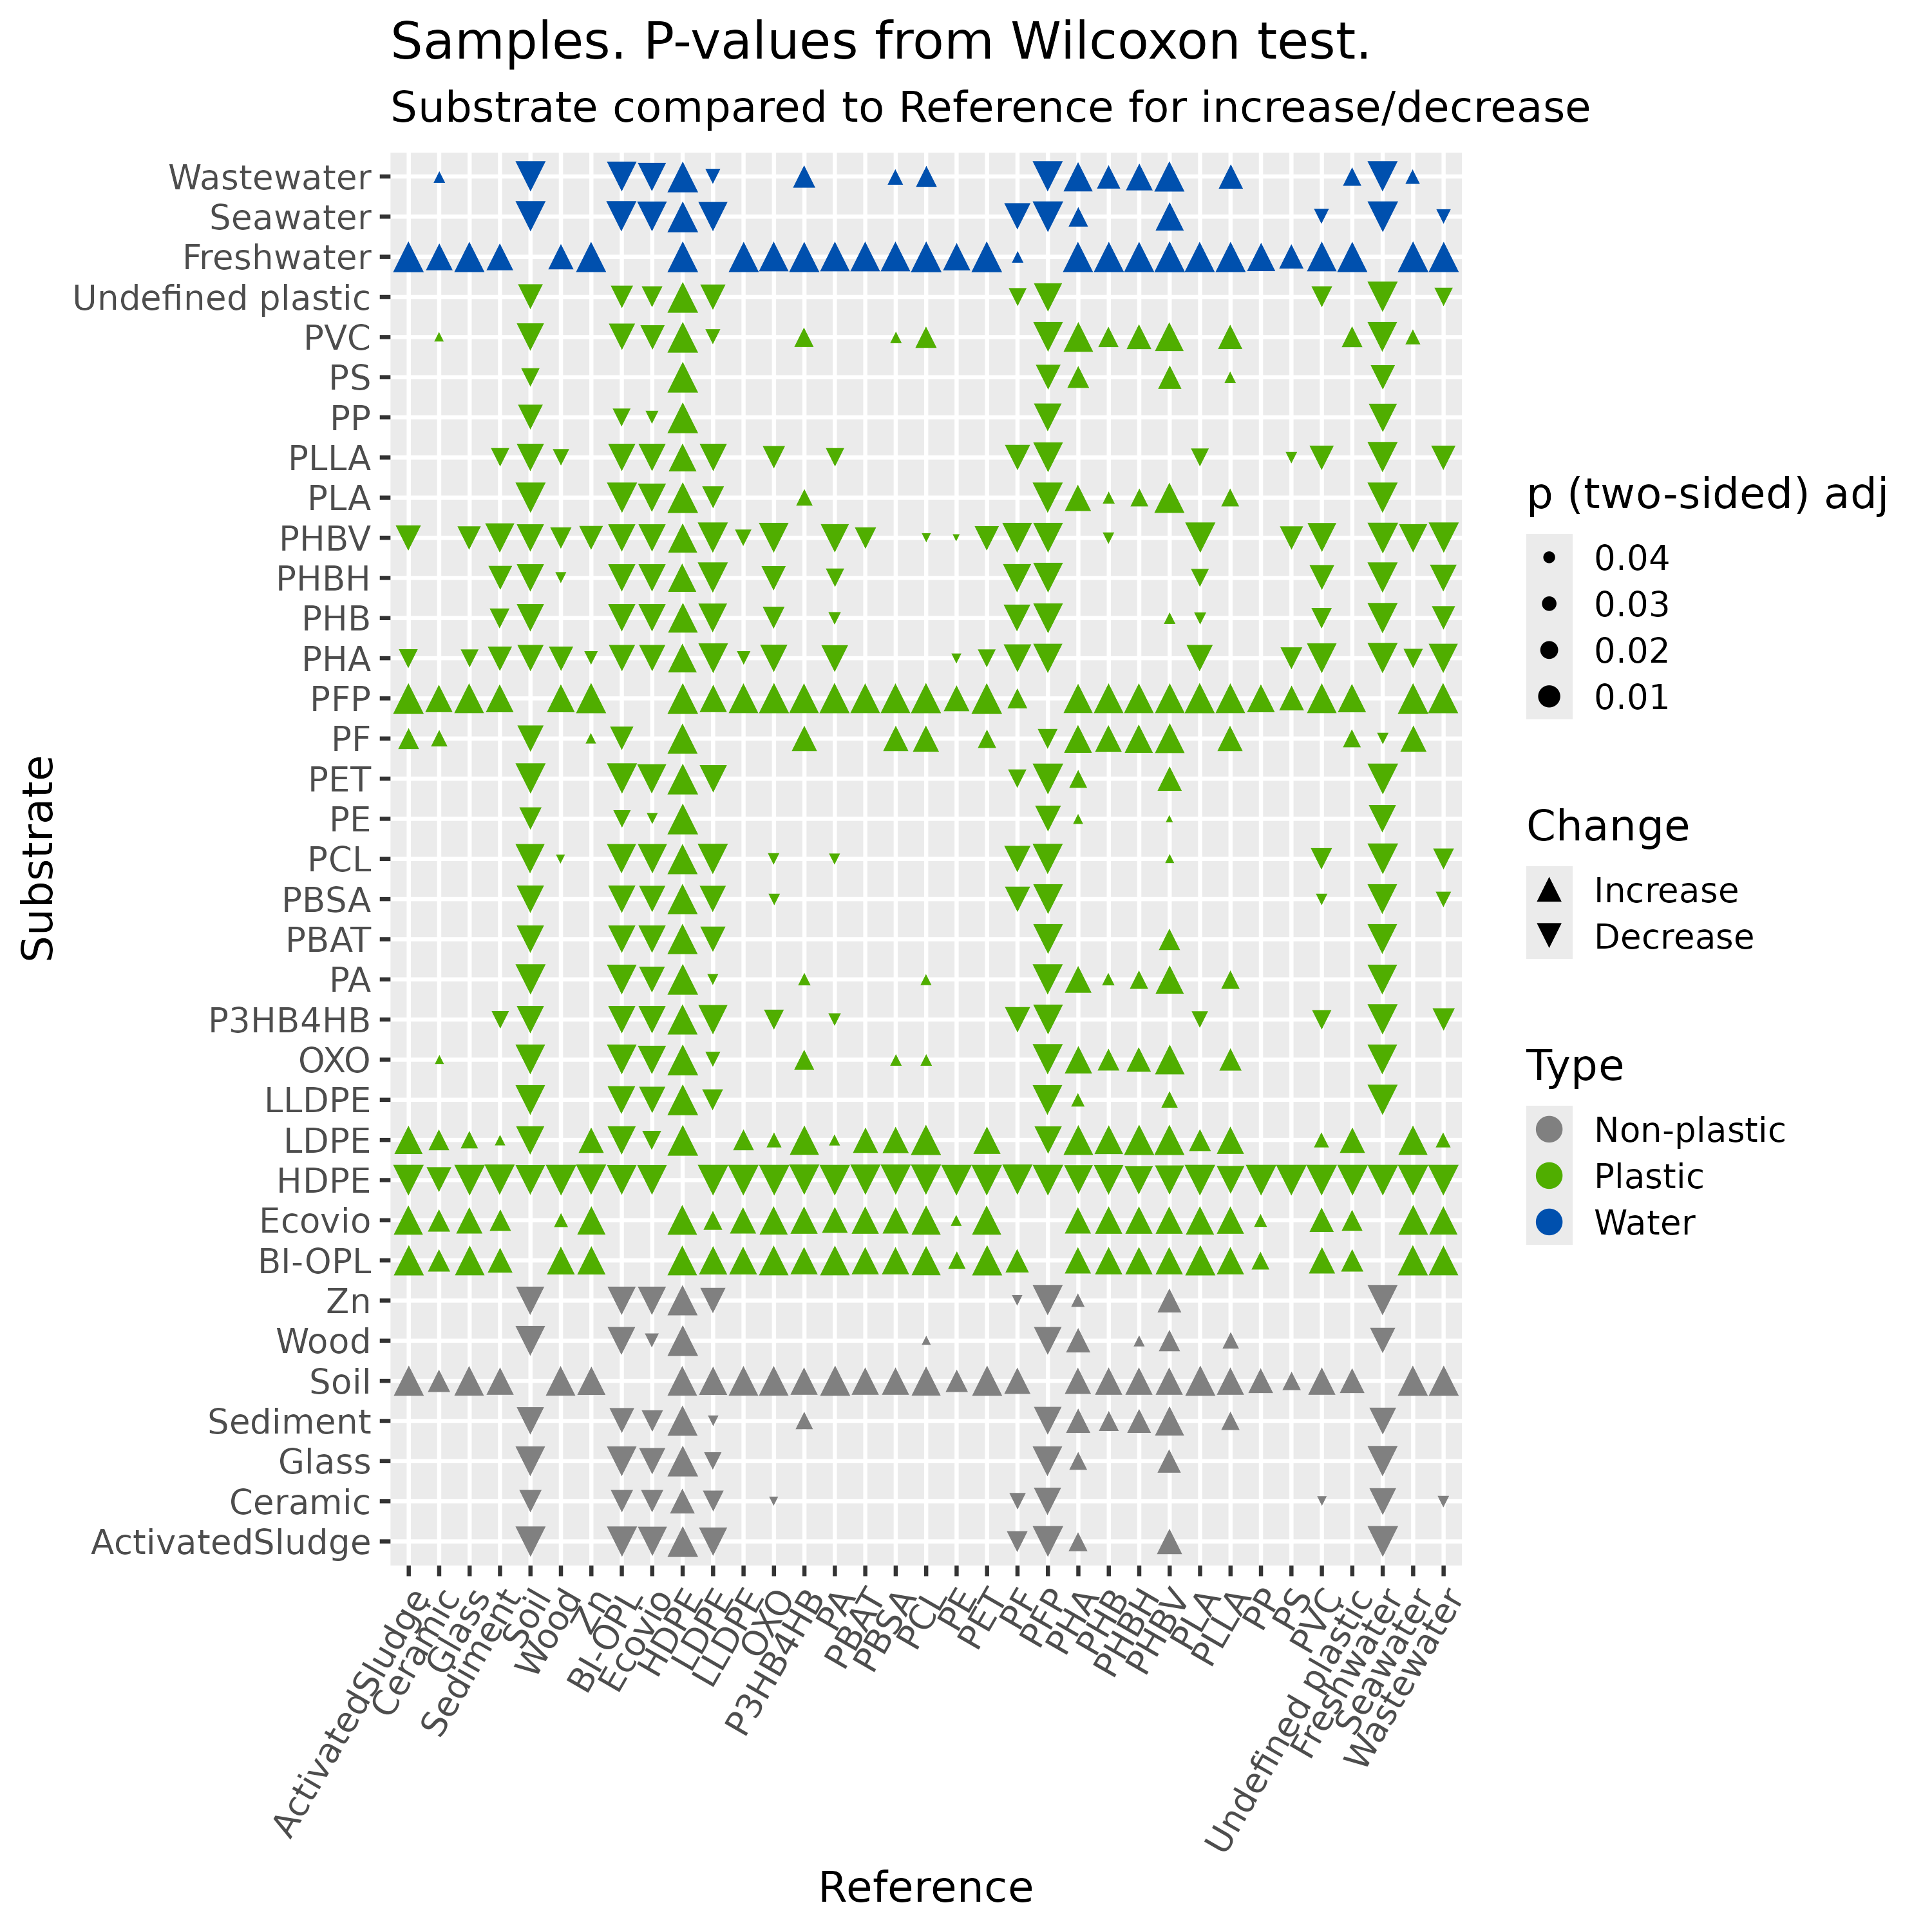
\includegraphics[width=0.5\textwidth]{figure/wilcox_samples_substrates.png}}
    \caption{(a) Mean mutation percentage per sample, grouped by substrate type. (b) p-values from Wilcoxon test of mean mutation percentage for Substrate versus Reference}
    \label{both_mean_samples_susbtrates}
\end{figure}

%\subsubsection{Alternative 2, separate plots instead of combined, see figure \ref{both_mean_samples_susbtrates}}
%\begin{figure}[h]
    % \centering
    % 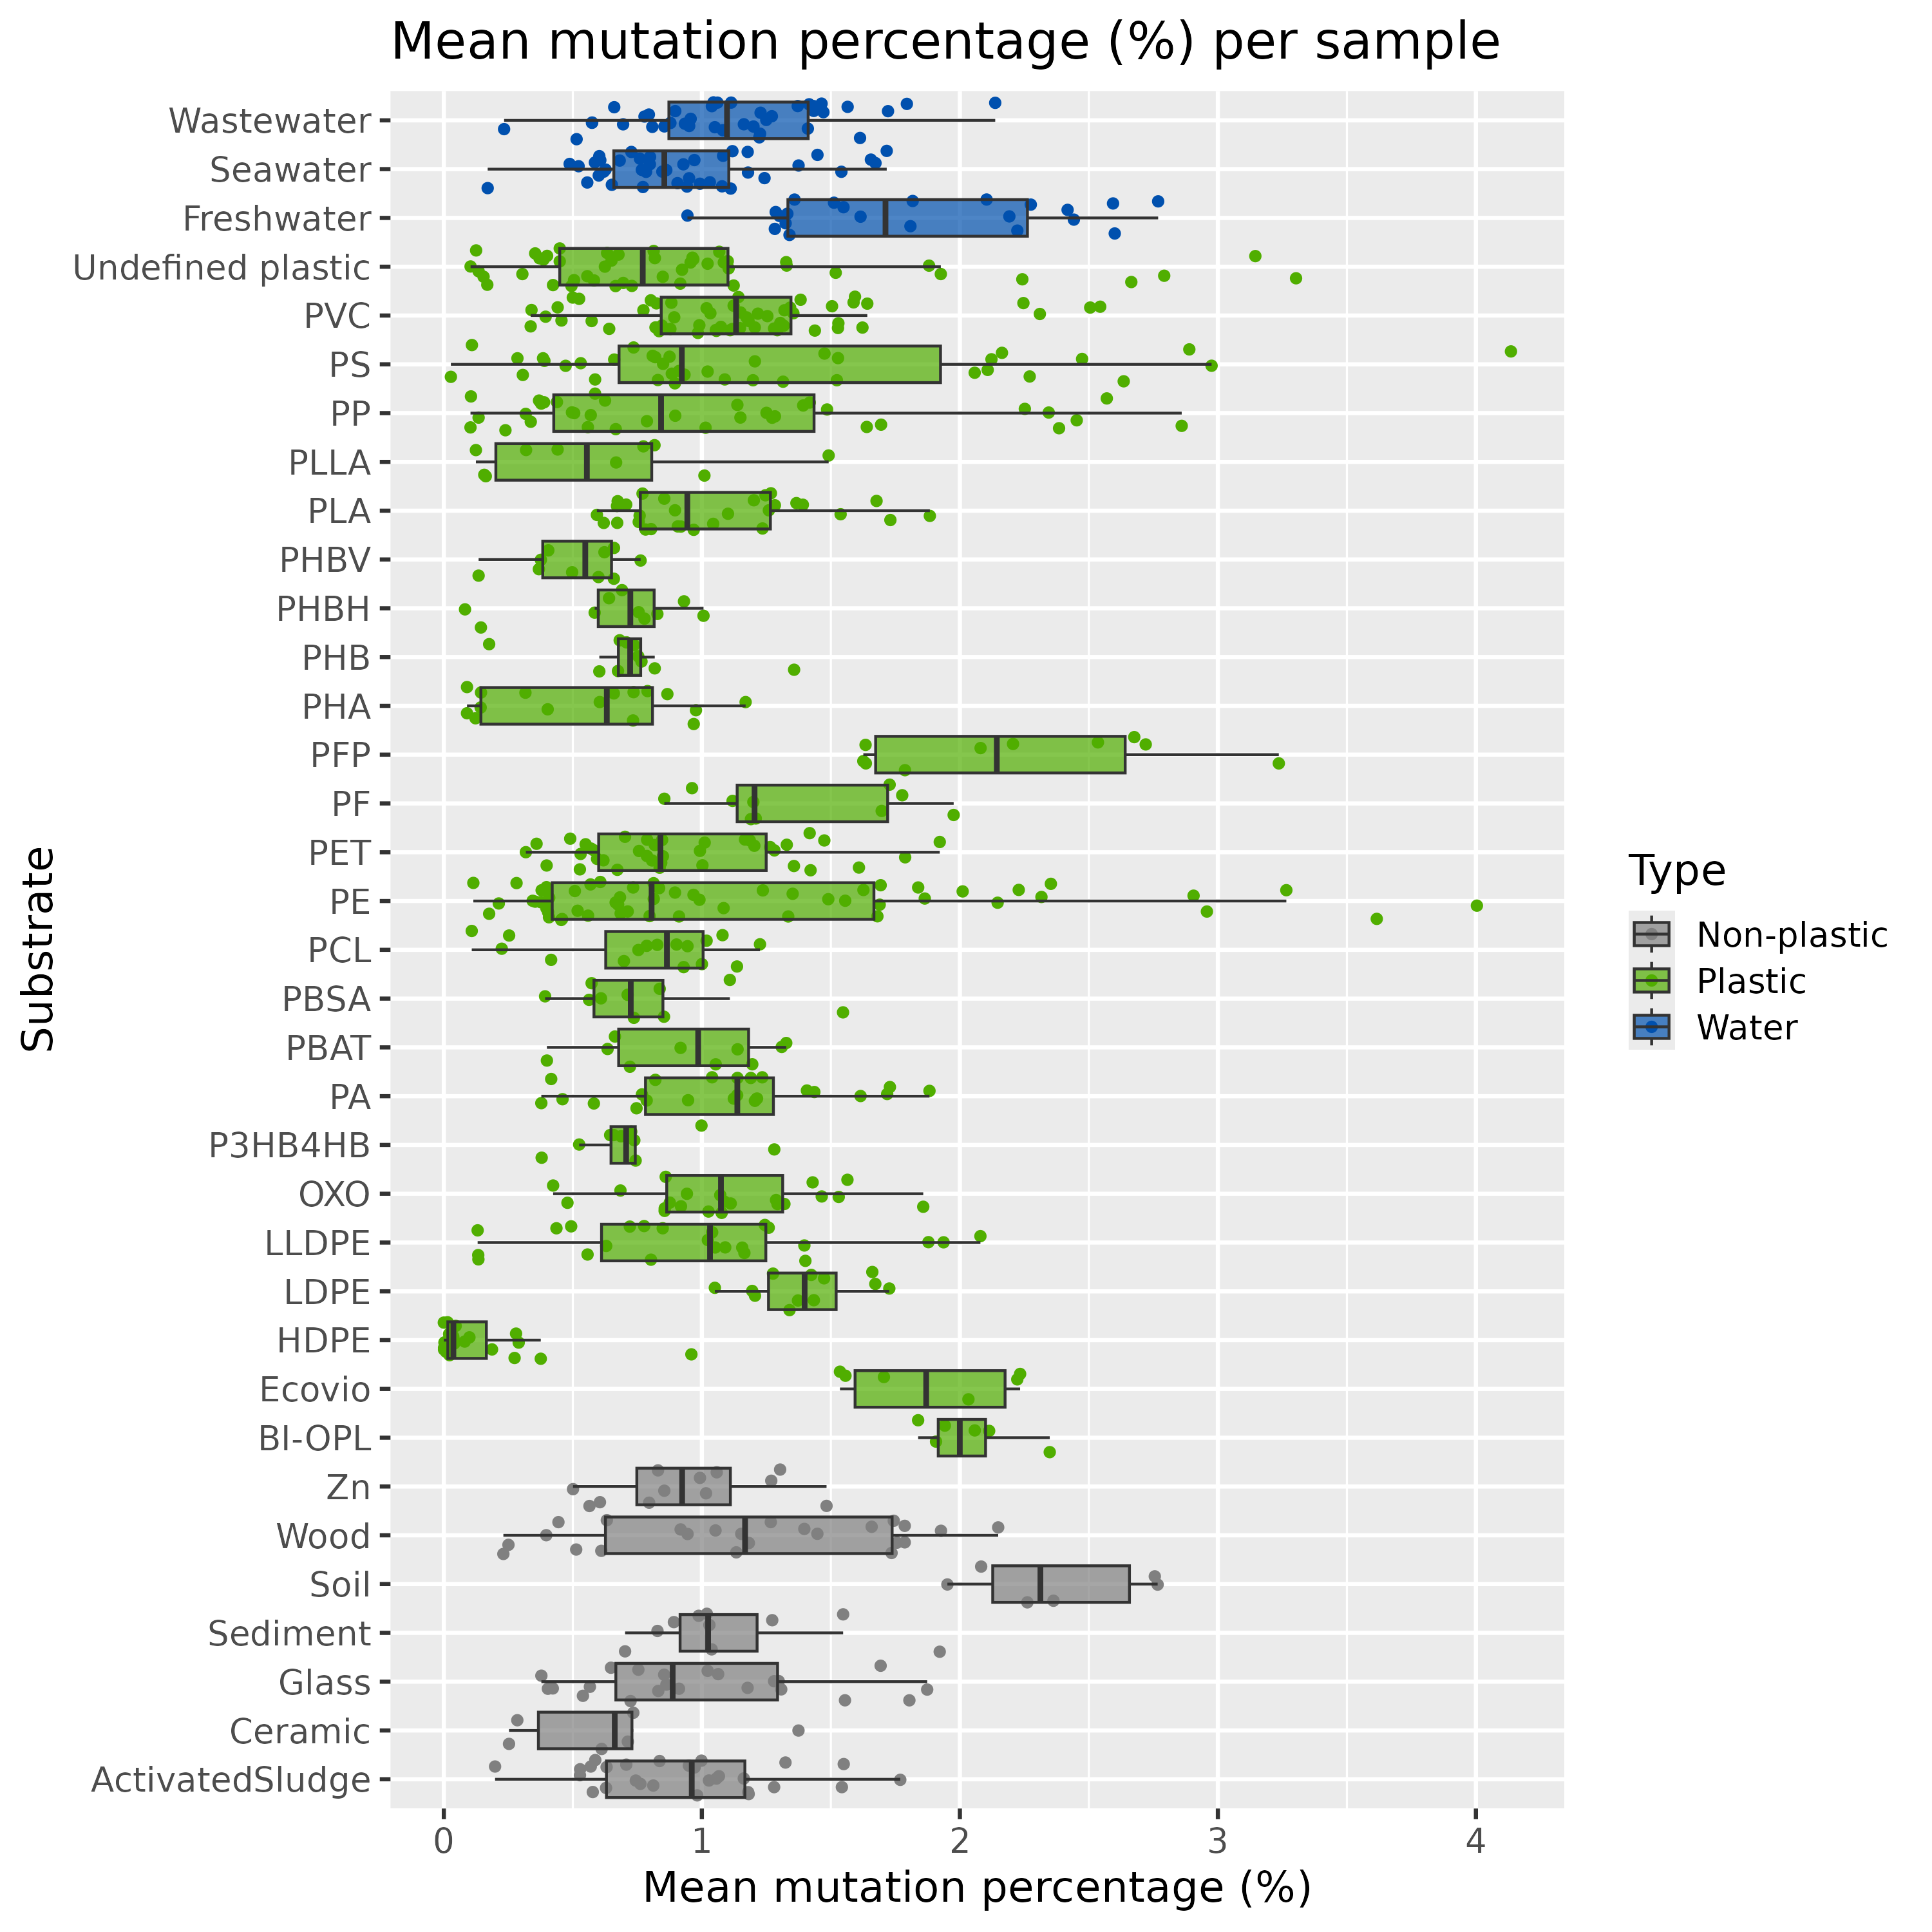
\includegraphics[width = 0.7\textwidth]{figure/mean_samples_substrate.png}
    % \caption{Mean Samples Substrate Full}
    % \label{mean_samples_substrate_full}
% \end{figure}
% 
% \begin{figure}[h]
    % \centering
    % 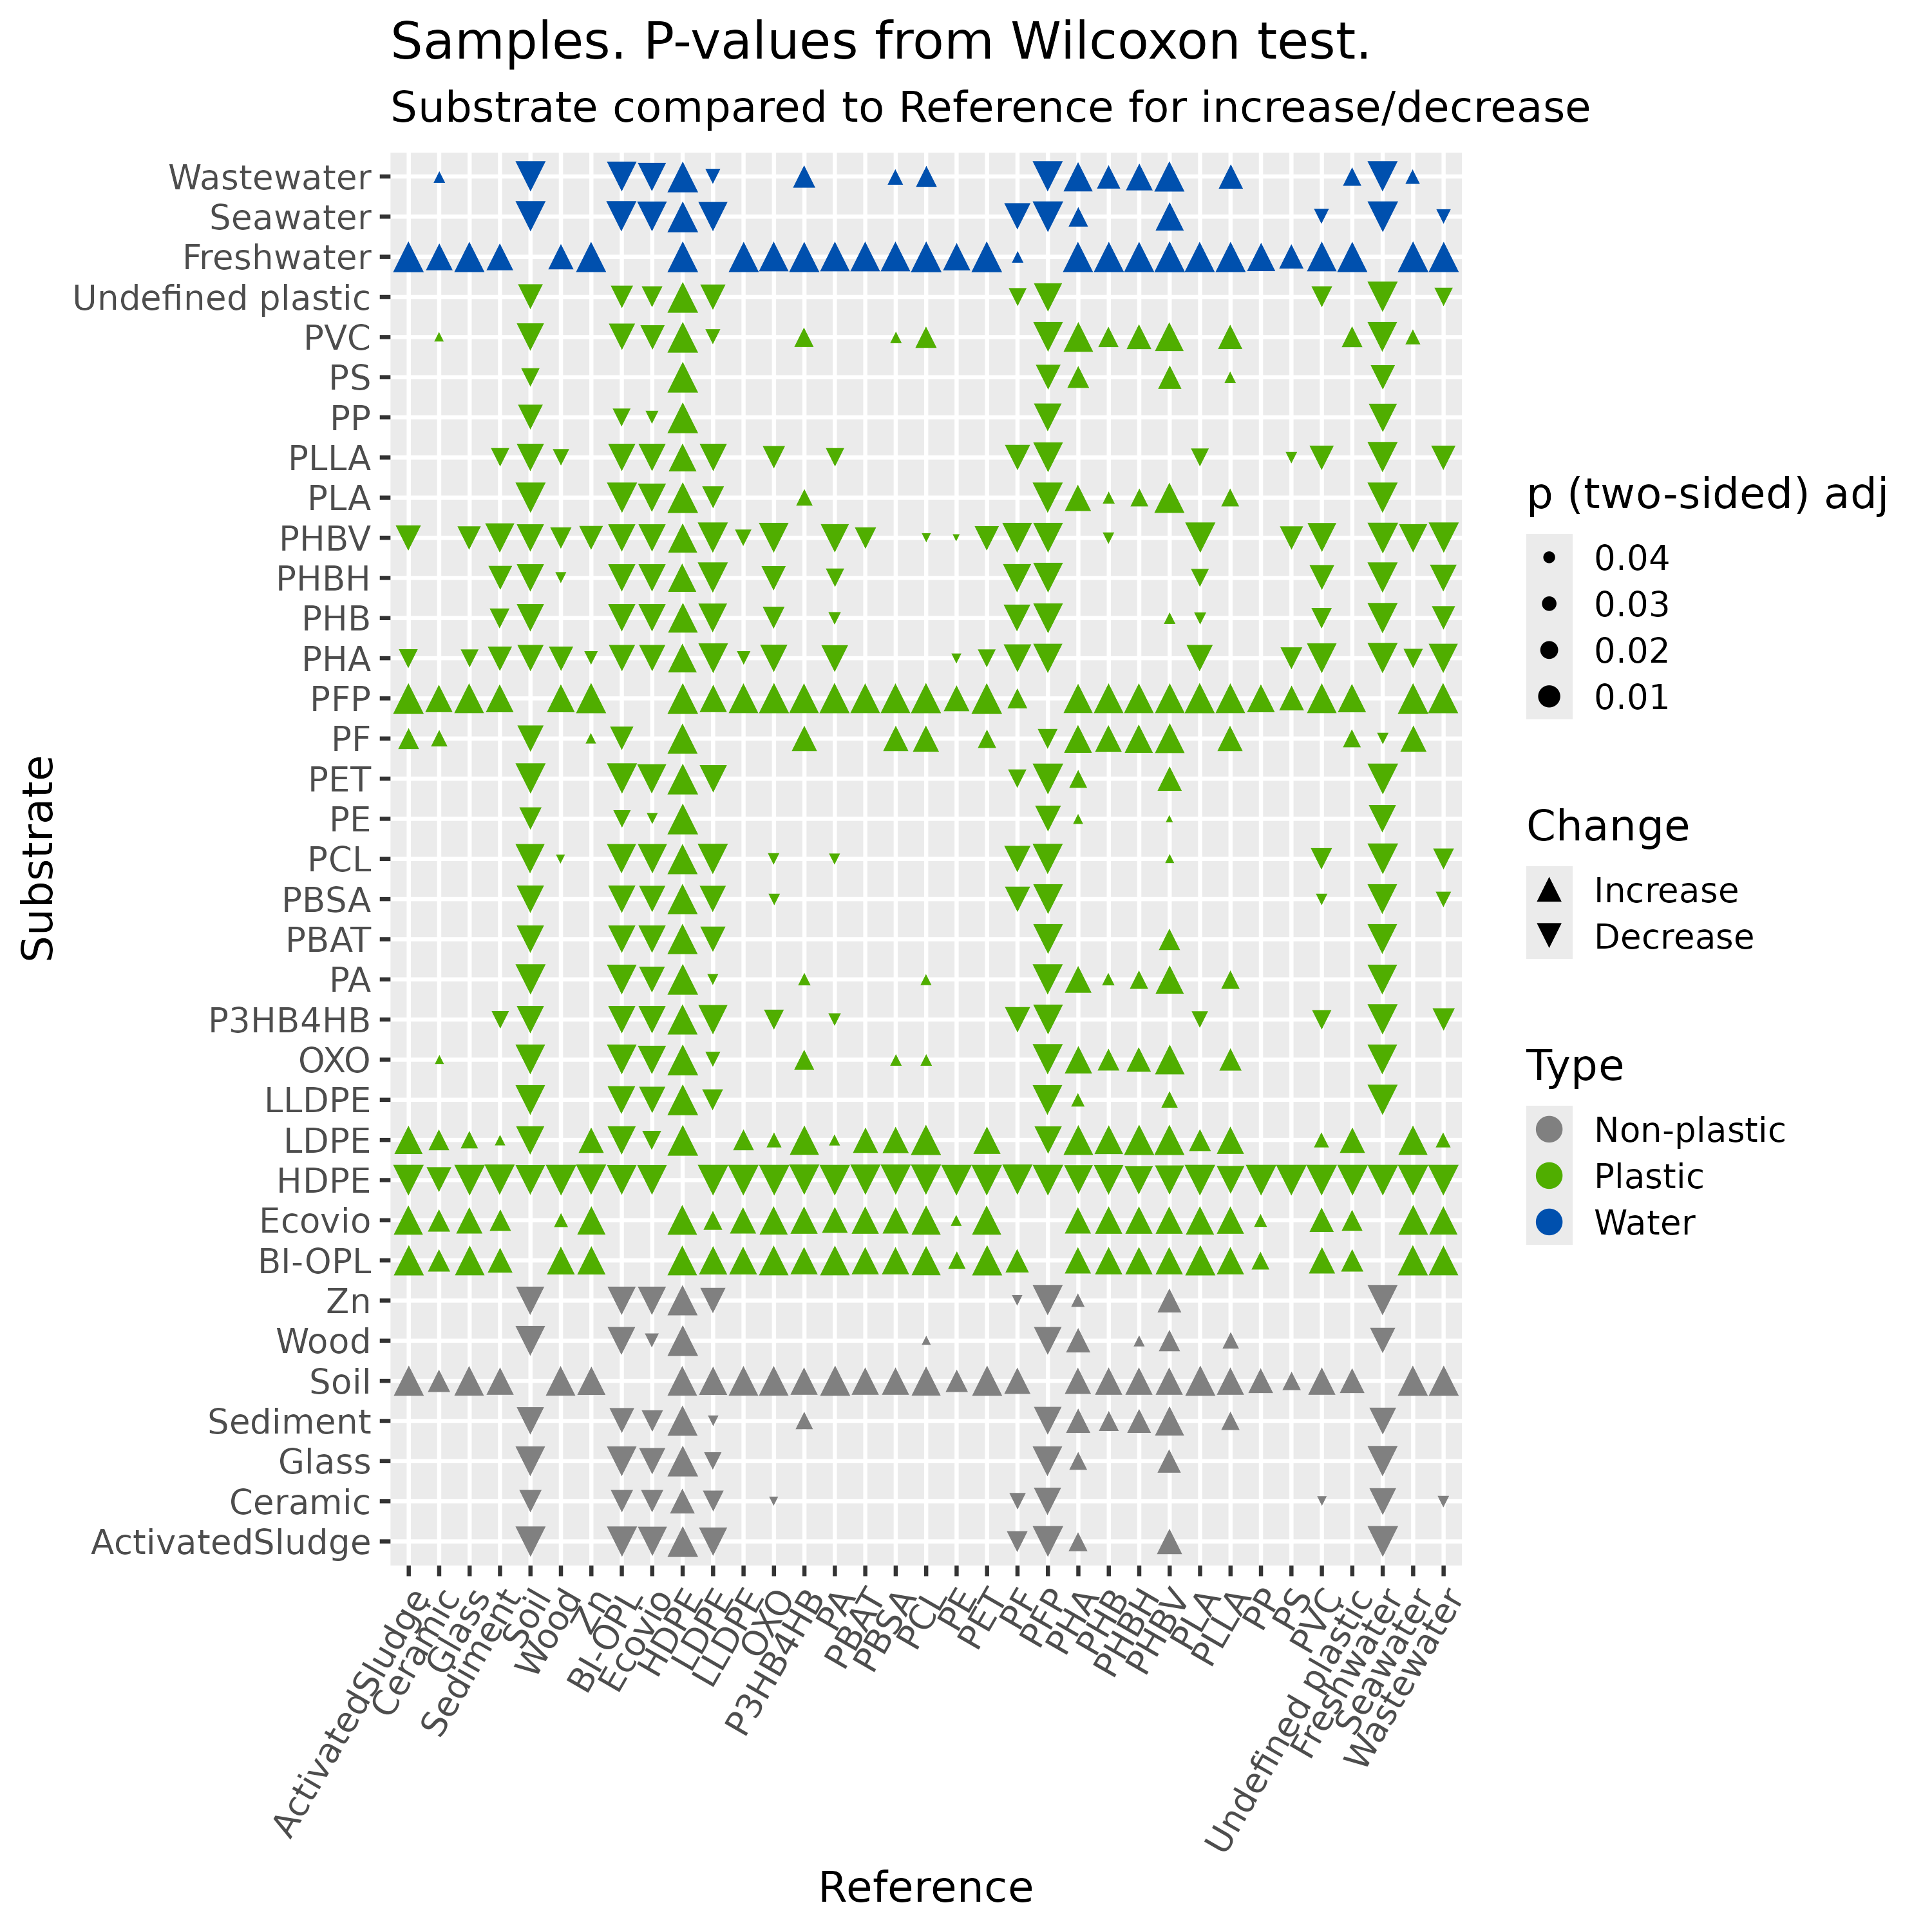
\includegraphics[width = 0.7\textwidth]{figure/wilcox_samples_substrates.png}
    % \caption{Wilcoxon Samples Substrate Full}
    % \label{wilcox_samples_substrates_full}
% \end{figure}
% 

%\subsection{Mean mutation percentage of individual mutations}
%Figure \ref{mean_genes_sampletype} show the result if instead of the mean mutation percentage for each sample was calculated, the mean mutation percentage per mutation, grouped by sampletype was calculated. \todo{i.e. mutation A12D parC for water: 10\%, A12D parC for plastic: 0\%, A12D parC for non-plastic: 3\%} 
%The resulting figure is hard to interpret since many of the genes will have a mean close to zero. If instead a log-scale was used, it removes many of the data points from the water and nonplastic groups, since they have a mean mutation percentage of zero. This skews the figure shown, and end up showing the reverse change as described below. \todo{Since we cannot use the log plot, do we need to use the bad plot instead, or can we skip it and just use stats?}
The mean mutation rate of individual point mutations grouped by sample type is shown in figure \ref{mean_genes_sampletype}. The mean mutation percentage was significantly different (p < 0.001) and higher for the plastic samples compared to both the water samples and the non-plastic samples. There is not a significant change between the water group and the non-plastic group.
% There is a significant difference between the different sample types, where plastic show an increase compared to both the water samples and the non-plastic samples.

\begin{figure}[h!]
    \centering
    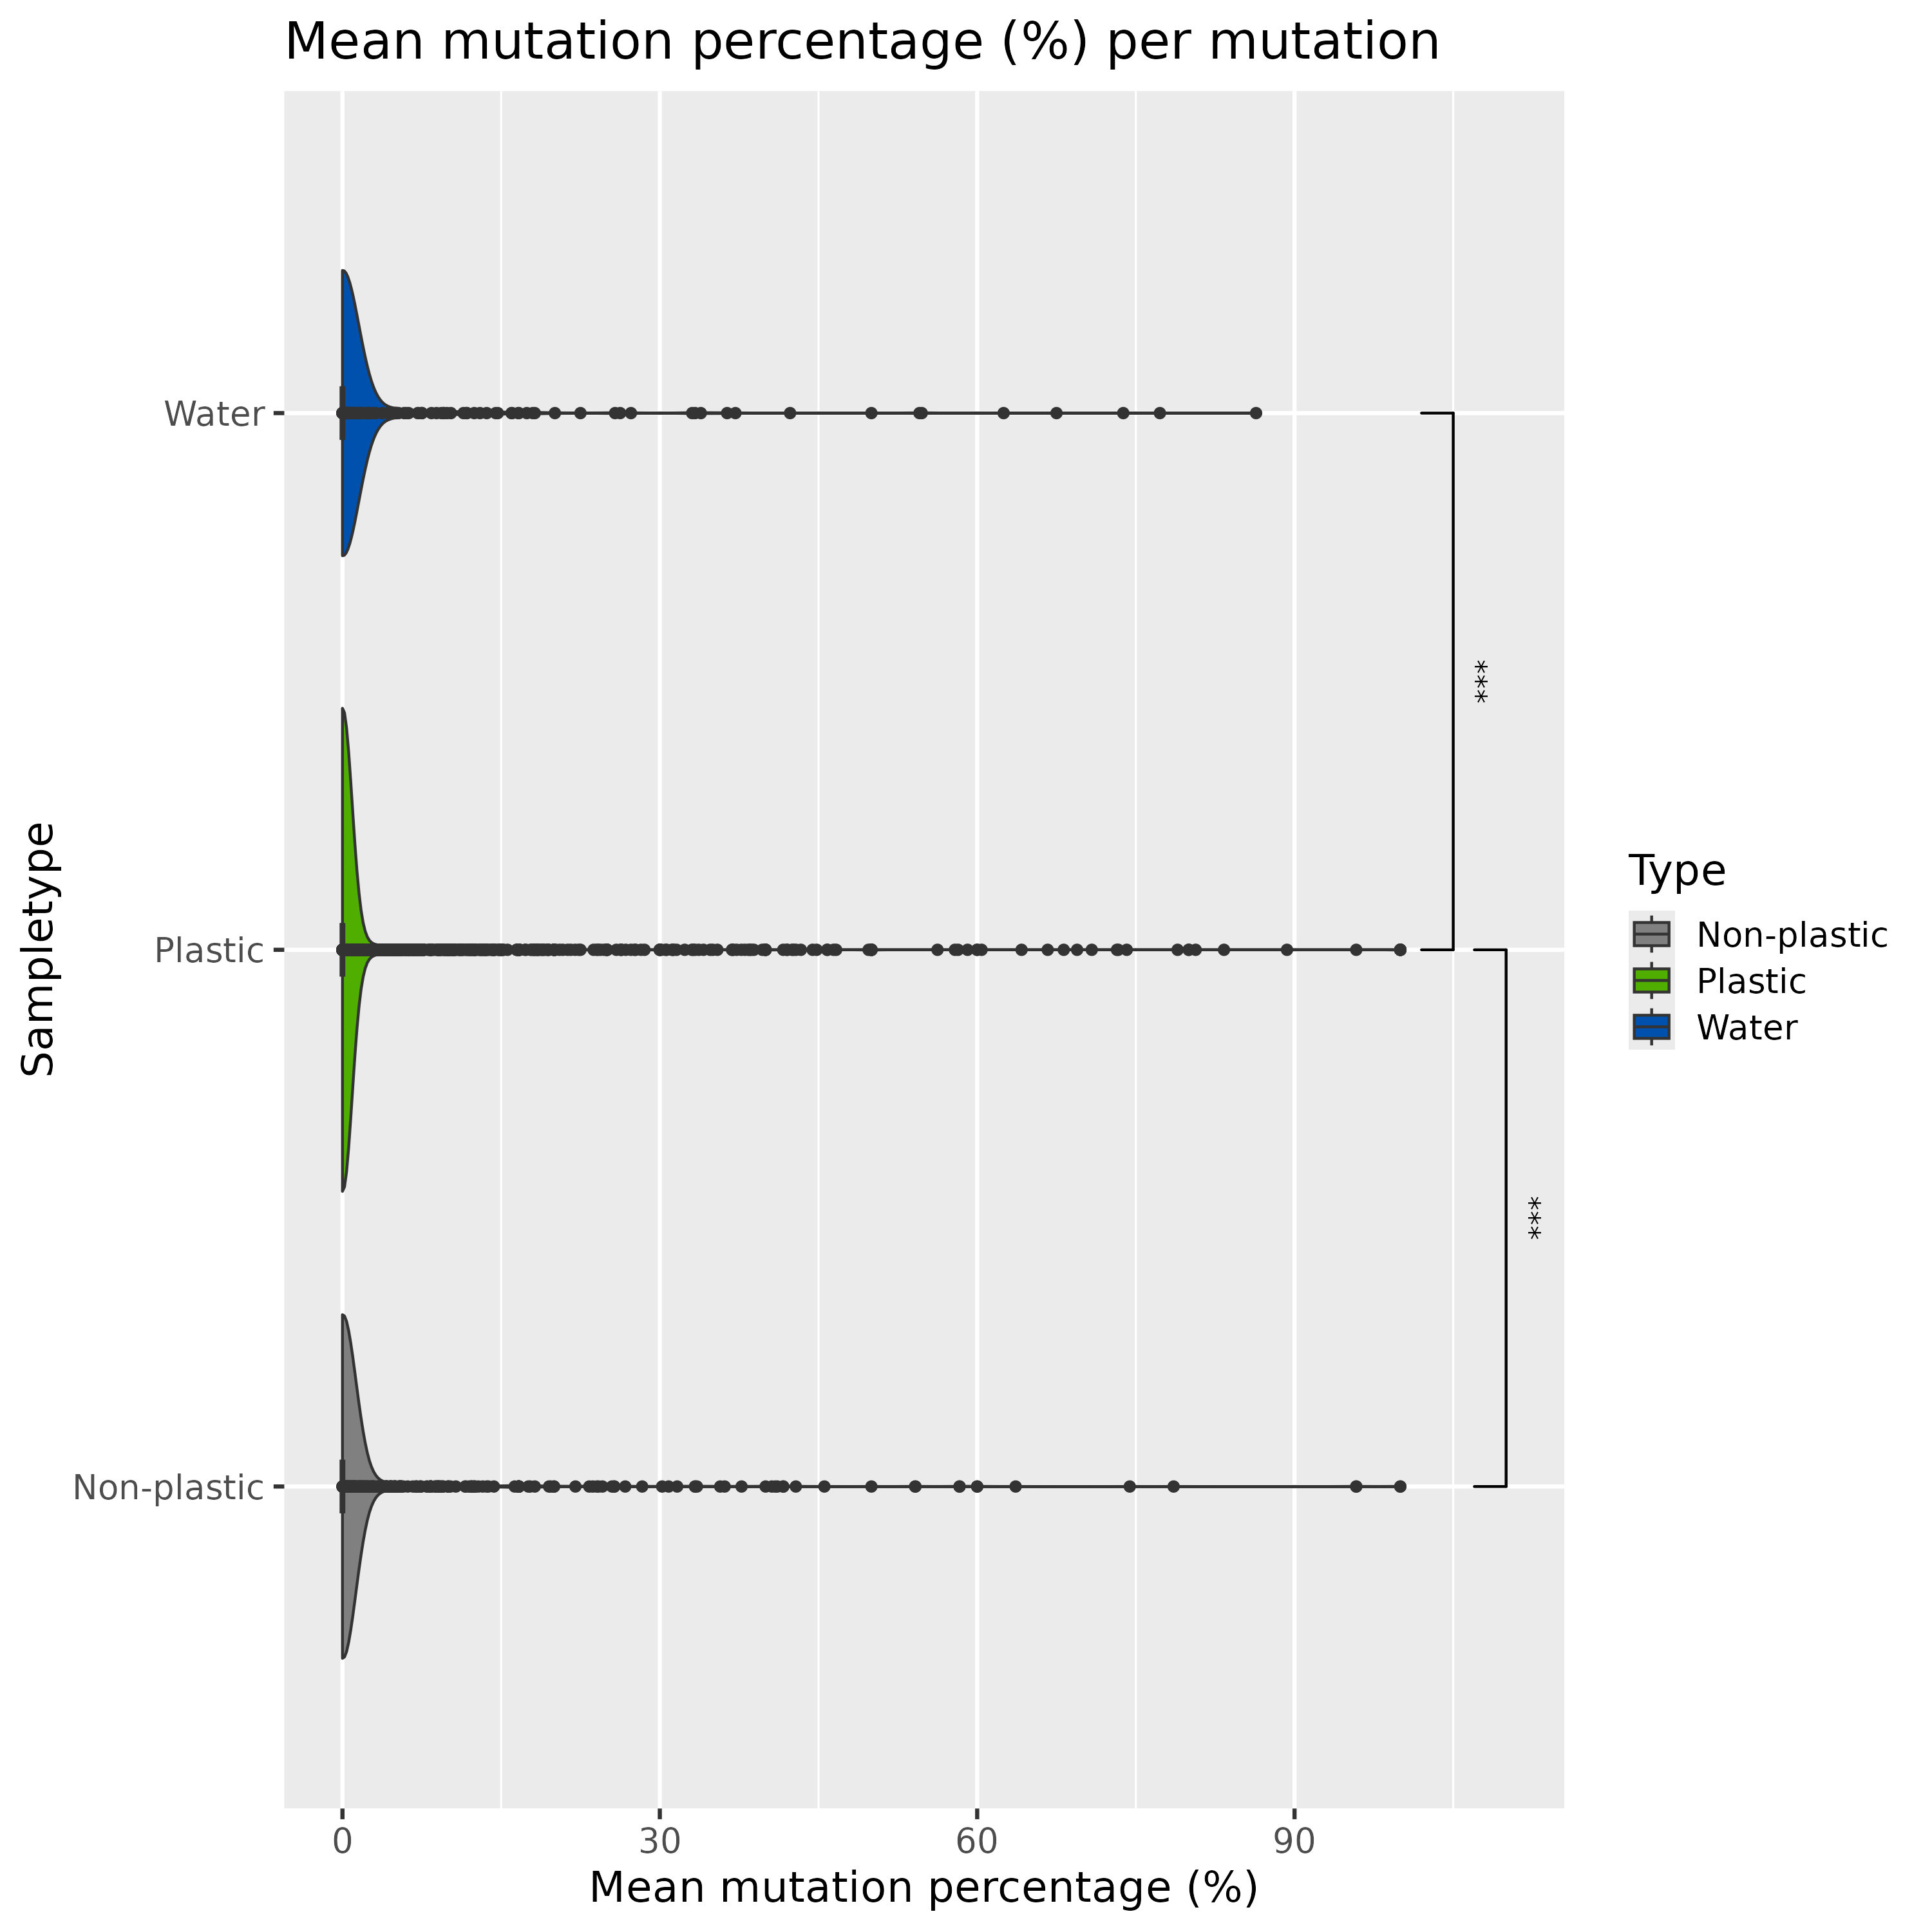
\includegraphics[width = 0.7\textwidth]{figure/mean_genes_sampletype.png}
    \caption{Mean mutation percentage (\%) per sample, grouped by sampletype. *** = p < 0.001}
    \label{mean_genes_sampletype}
\end{figure}

Figure \ref{mean_genes_substrate} show the mean mutation percentage per mutation grouped by substrate type. The figure shows that there are differences between the different substrates, and this is supported by figure \ref{wilcox_genes_substrate} which show the p-values from a Wilcoxon test between them, and that there are significant differences between many of them.
% Since figure \ref{mean_genes_substrate} uses a log-scale for visibility, the normal interpretation of the box-plot cannot be done since many points are erroneously removed, and therefore is only for visualizing the mutation rate.
The substrates which have the highest mean mutation percentage are PFP, PE, Ecovio, and BI-OPL from the plastic group as well as soil and wood from the non-plastic sampletypes. Freshwater had a significant increase to most other substrates.

% FROM samples substrates: 
% In figure \ref{mean_samples_substrate} the samples are instead grouped by substrate type, which show that there are differences for different plastics, as well as other substrates. Figure \ref{wilcox_samples_substrate} show the statistical significance of the comparison, when a wilcoxon test was done for the Substrate versus the Reference, as well as if there is an increase of the pseudo-mean compared to the reference. Note that all comparisons were done, but only the significant ones (p < 0.05) are shown. It is shown that there are some plastics that has a significant higher mean mutation percentage than most other substrates. These include PFP, LDPE, Ecovio and BI-OPL. The last two plastics are biodegradable plastics. The plastic substrates that has a significant higher mean mutation percentage than seawater or wastewater include PVC and PF in addition to the other plastics mentioned before. There are also some plastics which have significantly different lower mean mutation percentage than almost all other substrates, the most notable of which is high-density polyethylene (HDPE), poly(3-hydroxybutyrate-co-3-hydroxyvalerate) (PHBV) and polyhydroxyalkanoate (PHA), of which the latter two are biodegradable polymers while the first one is not. Almost all substrates has a significantly different lower mean mutation percentage than the freshwater samples, the exception of which is leaf, rock, Ecovio, BI-OPL, and PFP where there is no significant difference. The soil samples also has a significant higher mean mutation percentage compared to many other substrates.

\begin{figure}[h!]
    \centering
    \subfloat[\label{mean_genes_substrate}]{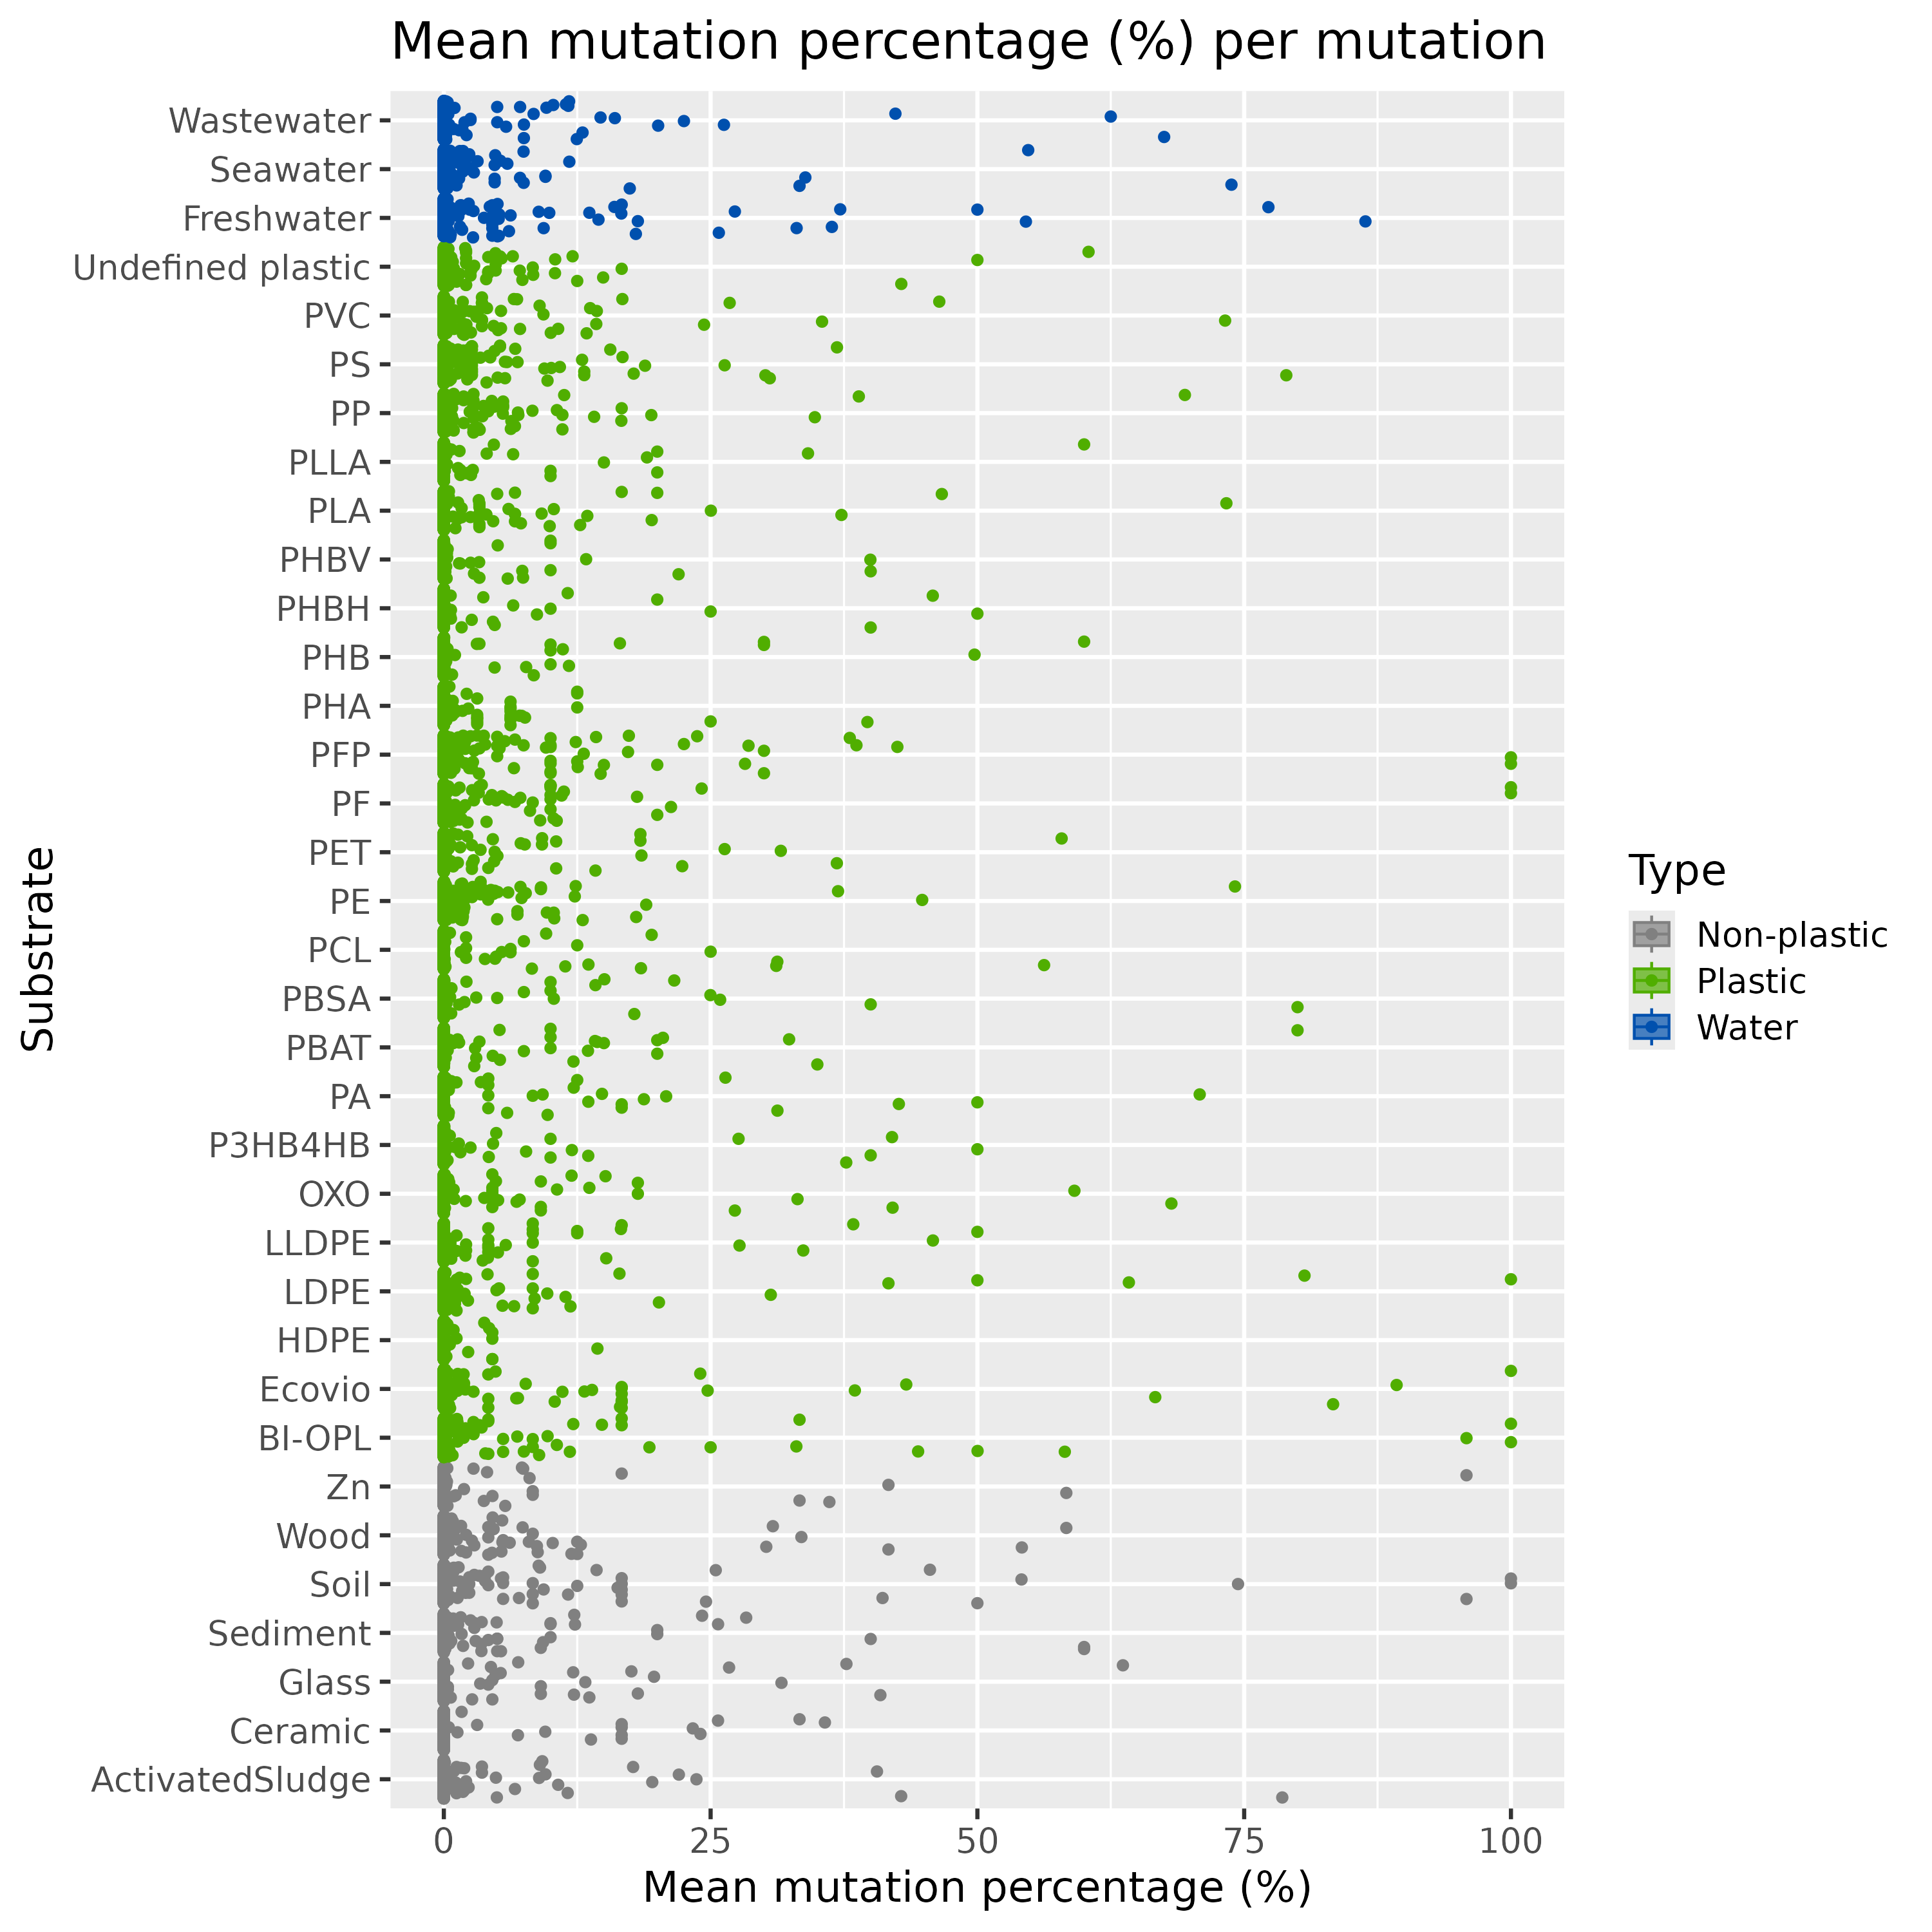
\includegraphics[width=0.5\textwidth]{figure/mean_genes_substrate.png}} 
    \subfloat[\label{wilcox_genes_substrate}]{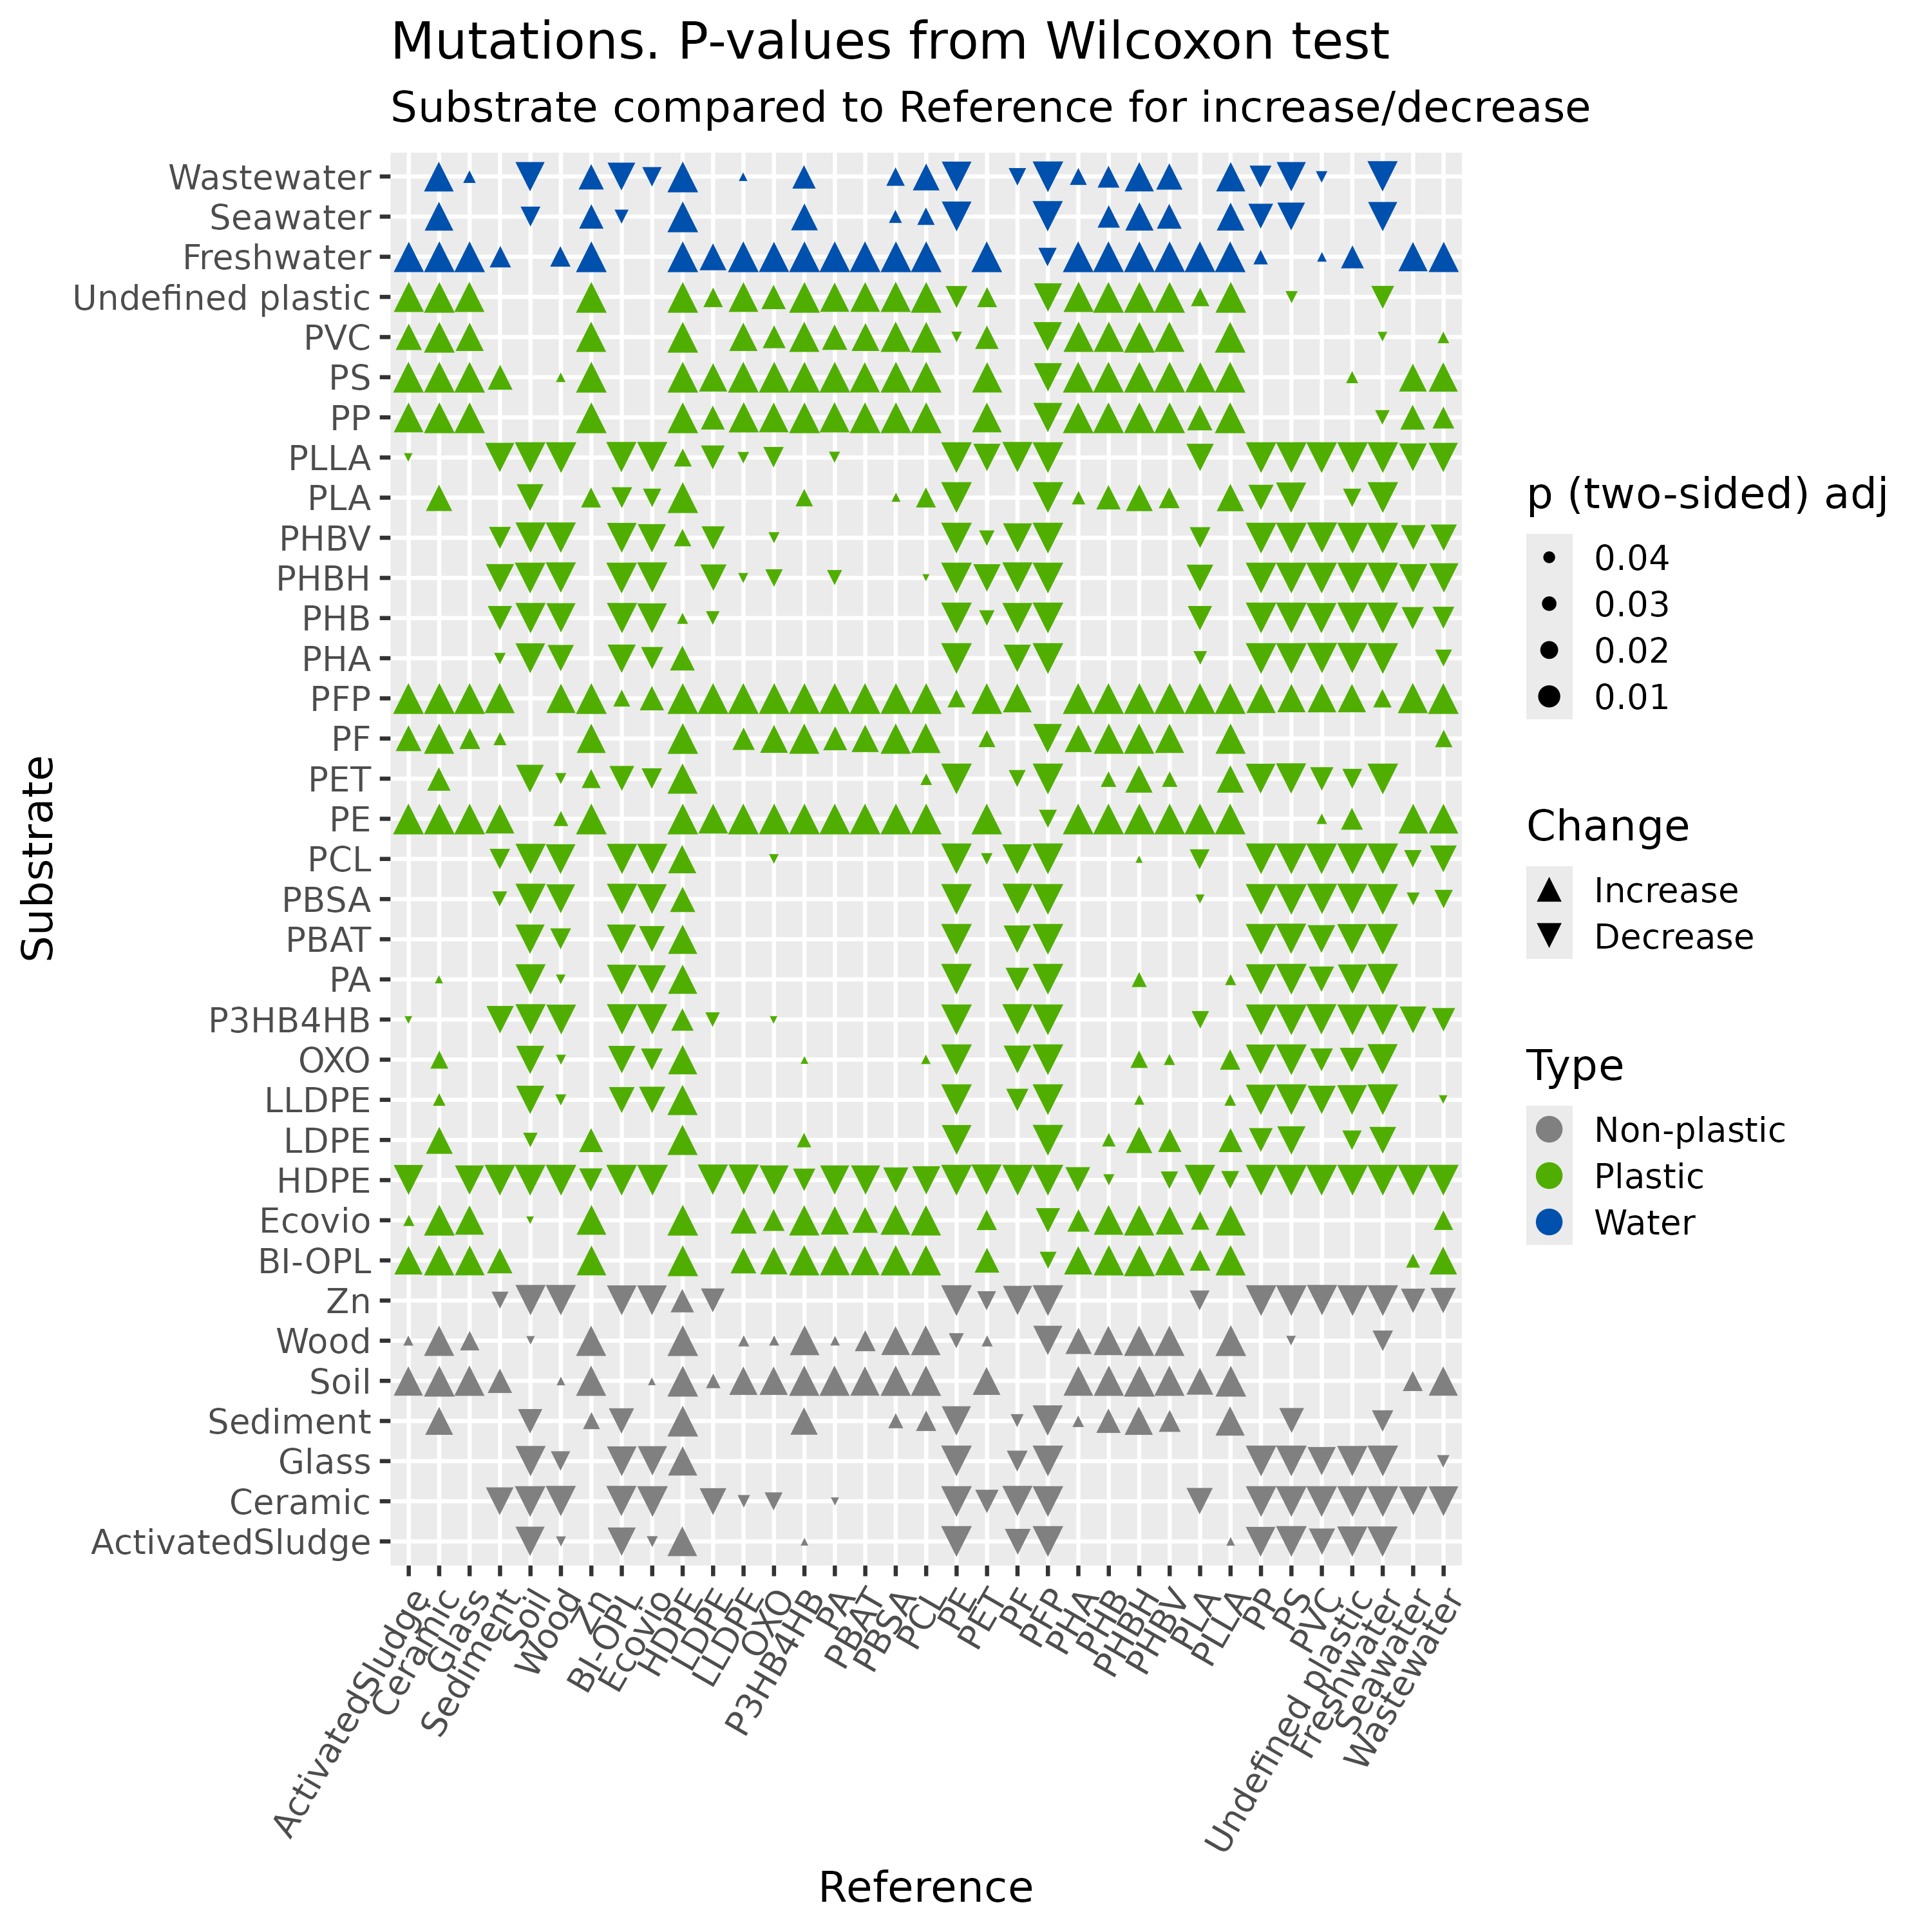
\includegraphics[width=0.5\textwidth]{figure/wilcox_genes_substrates.png}}
    \caption{(a) Mean mutation percentage per mutation, grouped by substrate type. (b) p-values from Wilcoxon test of mean mutation percentage for Substrate versus Reference}
    \label{both_mean_genes_substrate}
\end{figure}

Figure \ref{pointplot_mutations} show the mean mutation percentage for point mutations with a mean mutation percentage higher than 25 percent in any substrate. 
The figure shows that there are certain mutations which occur in most substrates and some that only ooccur in some substrates. The ones which occur in almost all samples are Q1073R in rpoB which confer resistance to rifampicin, G1245B in gyrB which confer resistance to aminocoumarin, and D244Y in rpoC which confer resistance to vancomycin. \todo{Mention Ecovio, BI-OPL, PFP, Freshwater, Soil with many point mutations of high mean mutation percentage?}

\begin{figure}[!h]
    \centering
    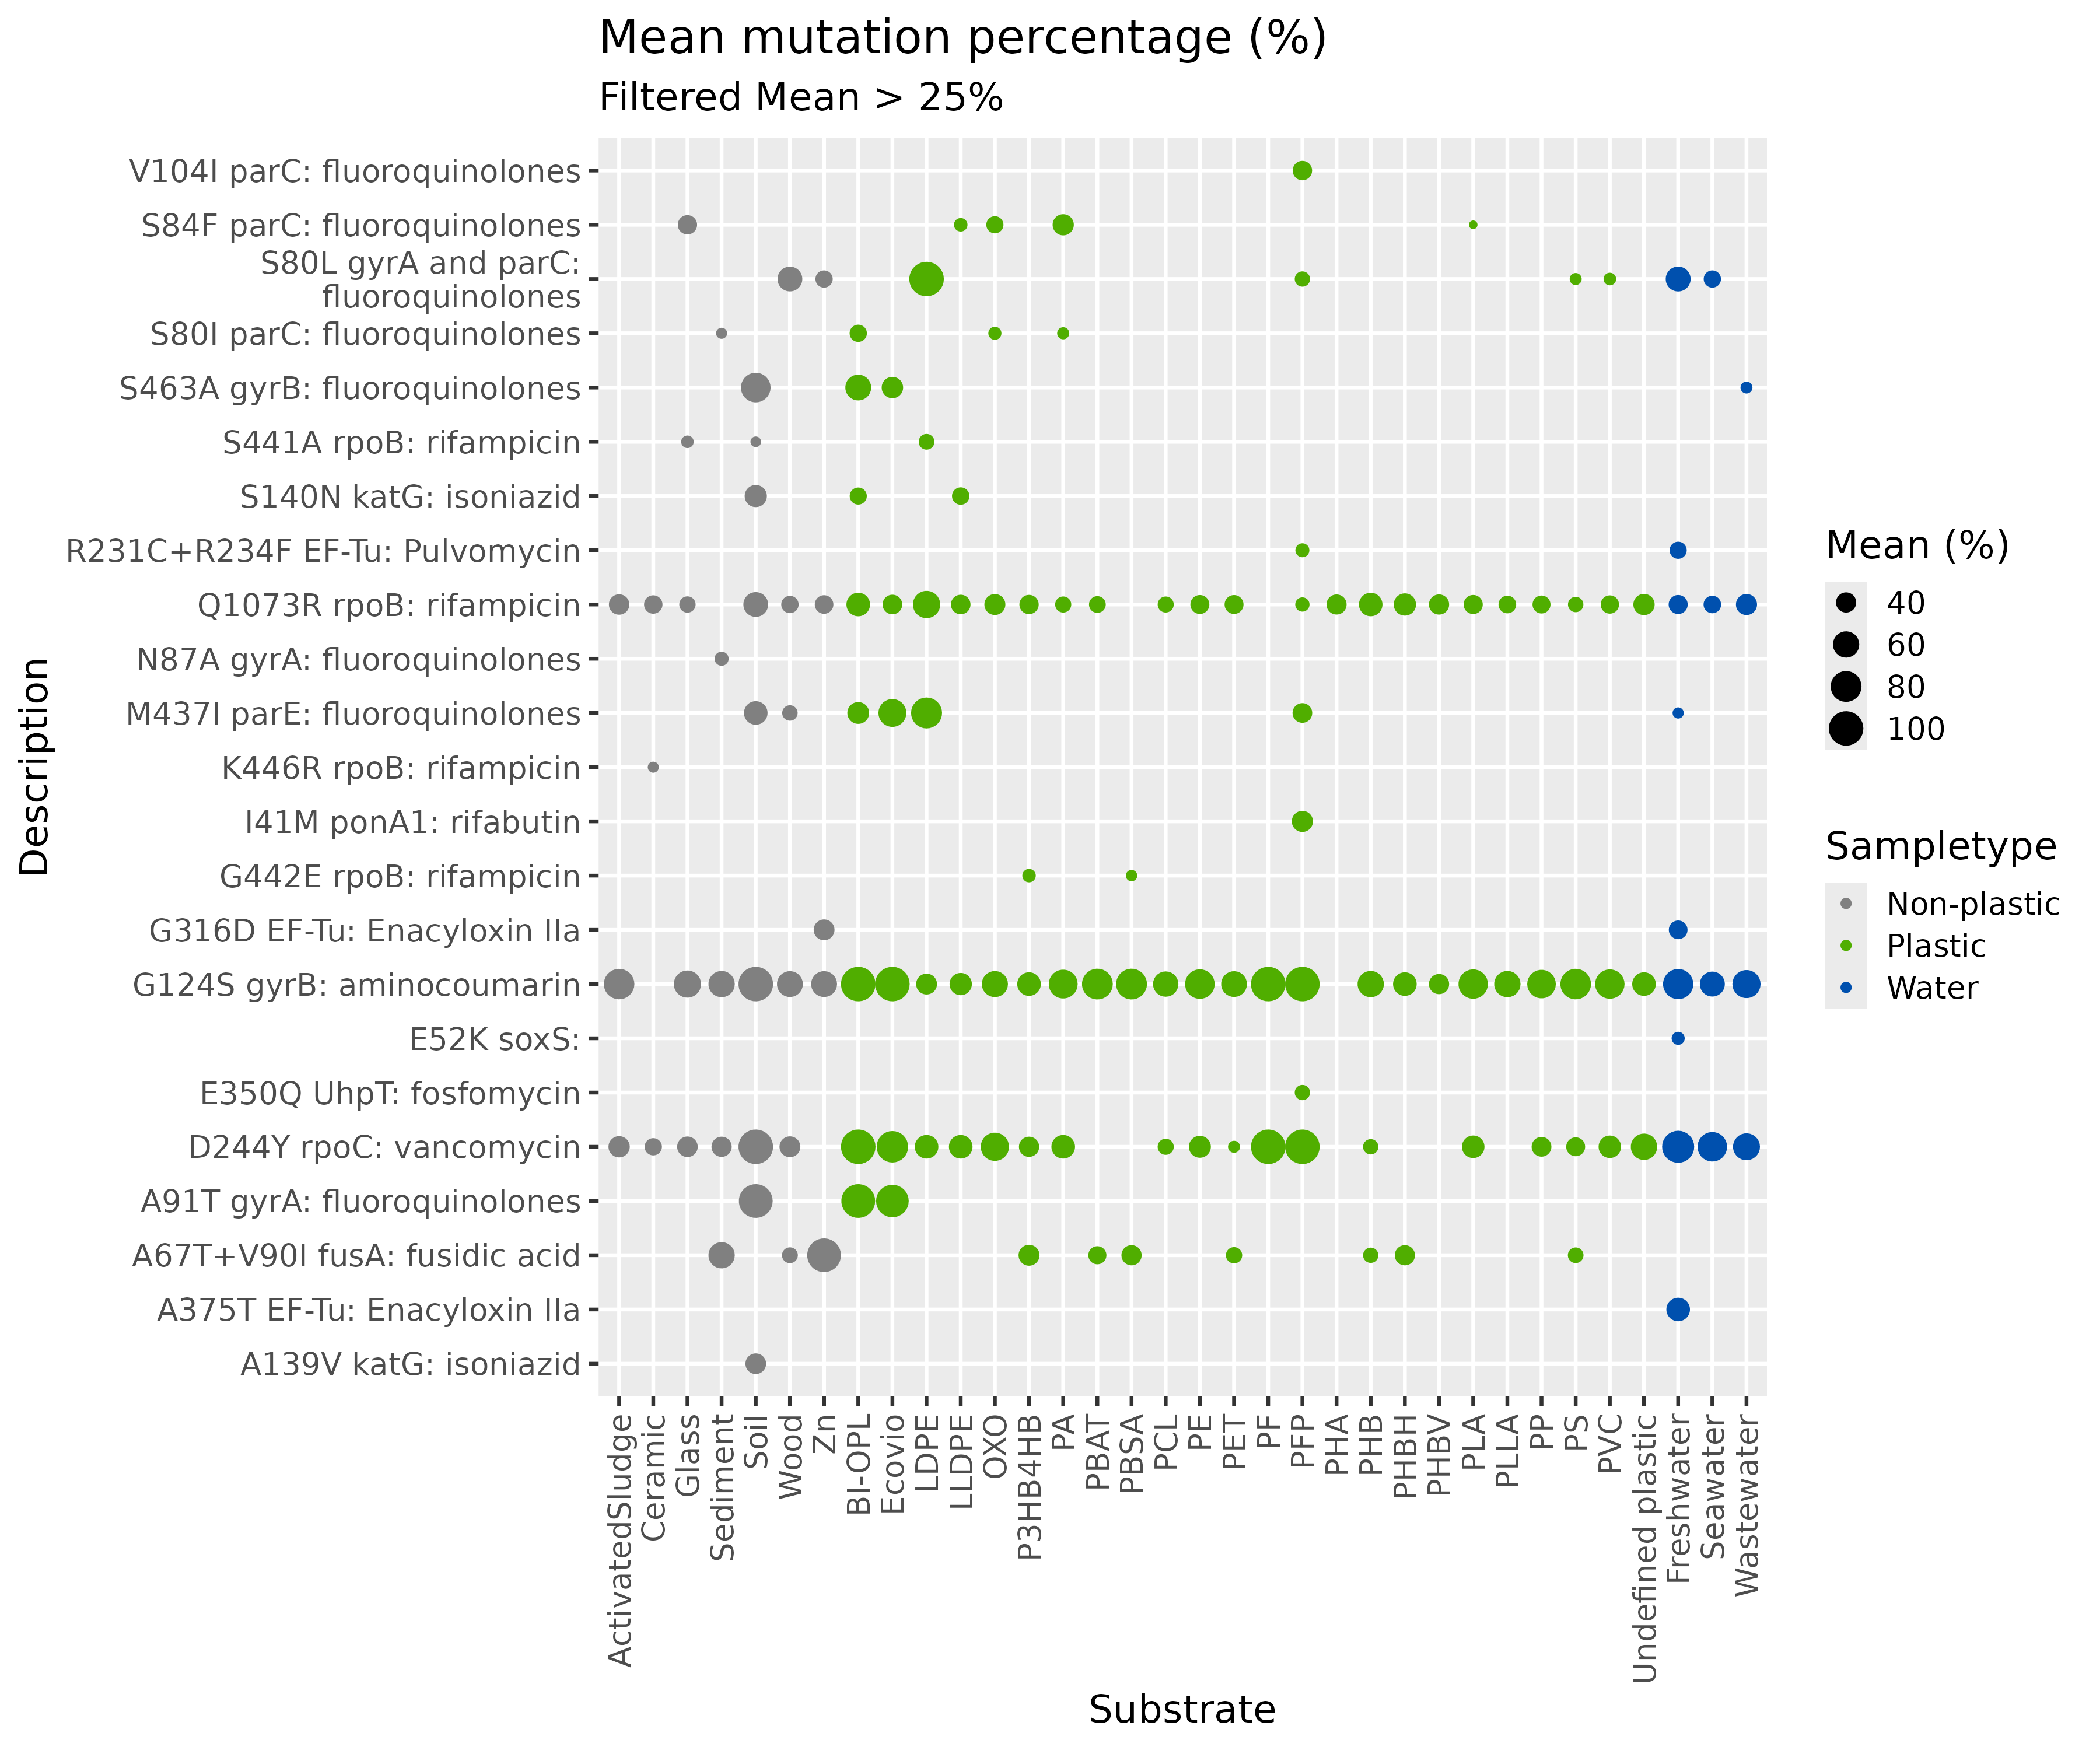
\includegraphics[width = \textwidth]{figure/relative_mean_points_25.png}
    \caption{Filtered mean mutation percentage per mutation. TODO: include this or skip?}
    \label{pointplot_mutations}
\end{figure}


\section{Predicting substrate identifiers} 
\todo{Rename from Random Forest to something else}
%TODO Rename to something else, "Predicting sample  
% Removed:
% D87H:Pseudomonas aeruginosa gyrA: fluoroquinolones
% D87H:Burkholderia dolosa gyrA: fluoroquinolones
%
% Renamed: There is one AMR Gene Family which has a very long name:
% "ATP-binding cassette (ABC) antibiotic efflux pump;General Bacterial Porin with reduced permeability to beta-lactams;major facilitator superfamily (MFS) antibiotic efflux pump;resistance-nodulation-cell division (RND) antibiotic efflux pump"
In the following figures only the ten most significant AMR Gene Families or mutations are shown. However, there are in all cases several more which are not shown. 
Figures showing all the 50 most significant variables can be found in Appendix \ref{appendix:code}.
\todo{Do this? Not sure if \emph{all} of them can be shown, but at least 50 is possible in a really long plot}

\subsection{AMR Gene Family}
In the database CARD, each mutation is associated with an AMR Gene Family, which is a classification tag such as "rifampicin resistant rpoC" or "fluoroquinolone resistant parC". The AMR Gene Family is used in this analysis since it enables us to group the mutations by gene and conferred antibiotic resistance.
%in order to identify the function of the mutations present in the samples.

%\subsubsection{Sampletypes}
Based on the mean decrease in Gini impurity, certain AMR Gene families were significantly (p < 0.001) assigned to the non-plastic sampletype, as shown in figure \ref{amr_sampletype}. These included fluoroquinolone resistant parC and gyrA as well as daptomycin-resistant beta-subunit of RNA polymerase (rpoB). 
%Figure \ref{amr_sampletype_bar} show the mean decrease in Gini impurity for five different AMR Gene Families, which was found to be significant.
%{true or not? true since kruskal-wallace test found X taxa singificant} when the samples are grouped by sampletype.
%Three of the families may be used to identify the non-plastic samples, which include fluoroquinolone resistant parC and gyrA as well as daptomycin-resistant beta-subunit of RNA polymerase (rpoB). 
The two significant AMR Gene Families for the water samples were vancomycin-resistant beta prime subunit of RNA polymerase (rpoC) and rifampicin-reistant rpoC. 
However, note the negative sign of these which indicate that these AMR Gene Families are more important to determine that a sample is in the reference group (the other groups) than in the water group. 
%\{It is significant, shows that a samples is NOT in the water group. As mentioned above. Can only say that a sample is from the non-plastic group, or NOT in the water group, not the abundance of it.}

\begin{figure}[h]
    \centering
    \subfloat[\label{amr_sampletype_bar}]{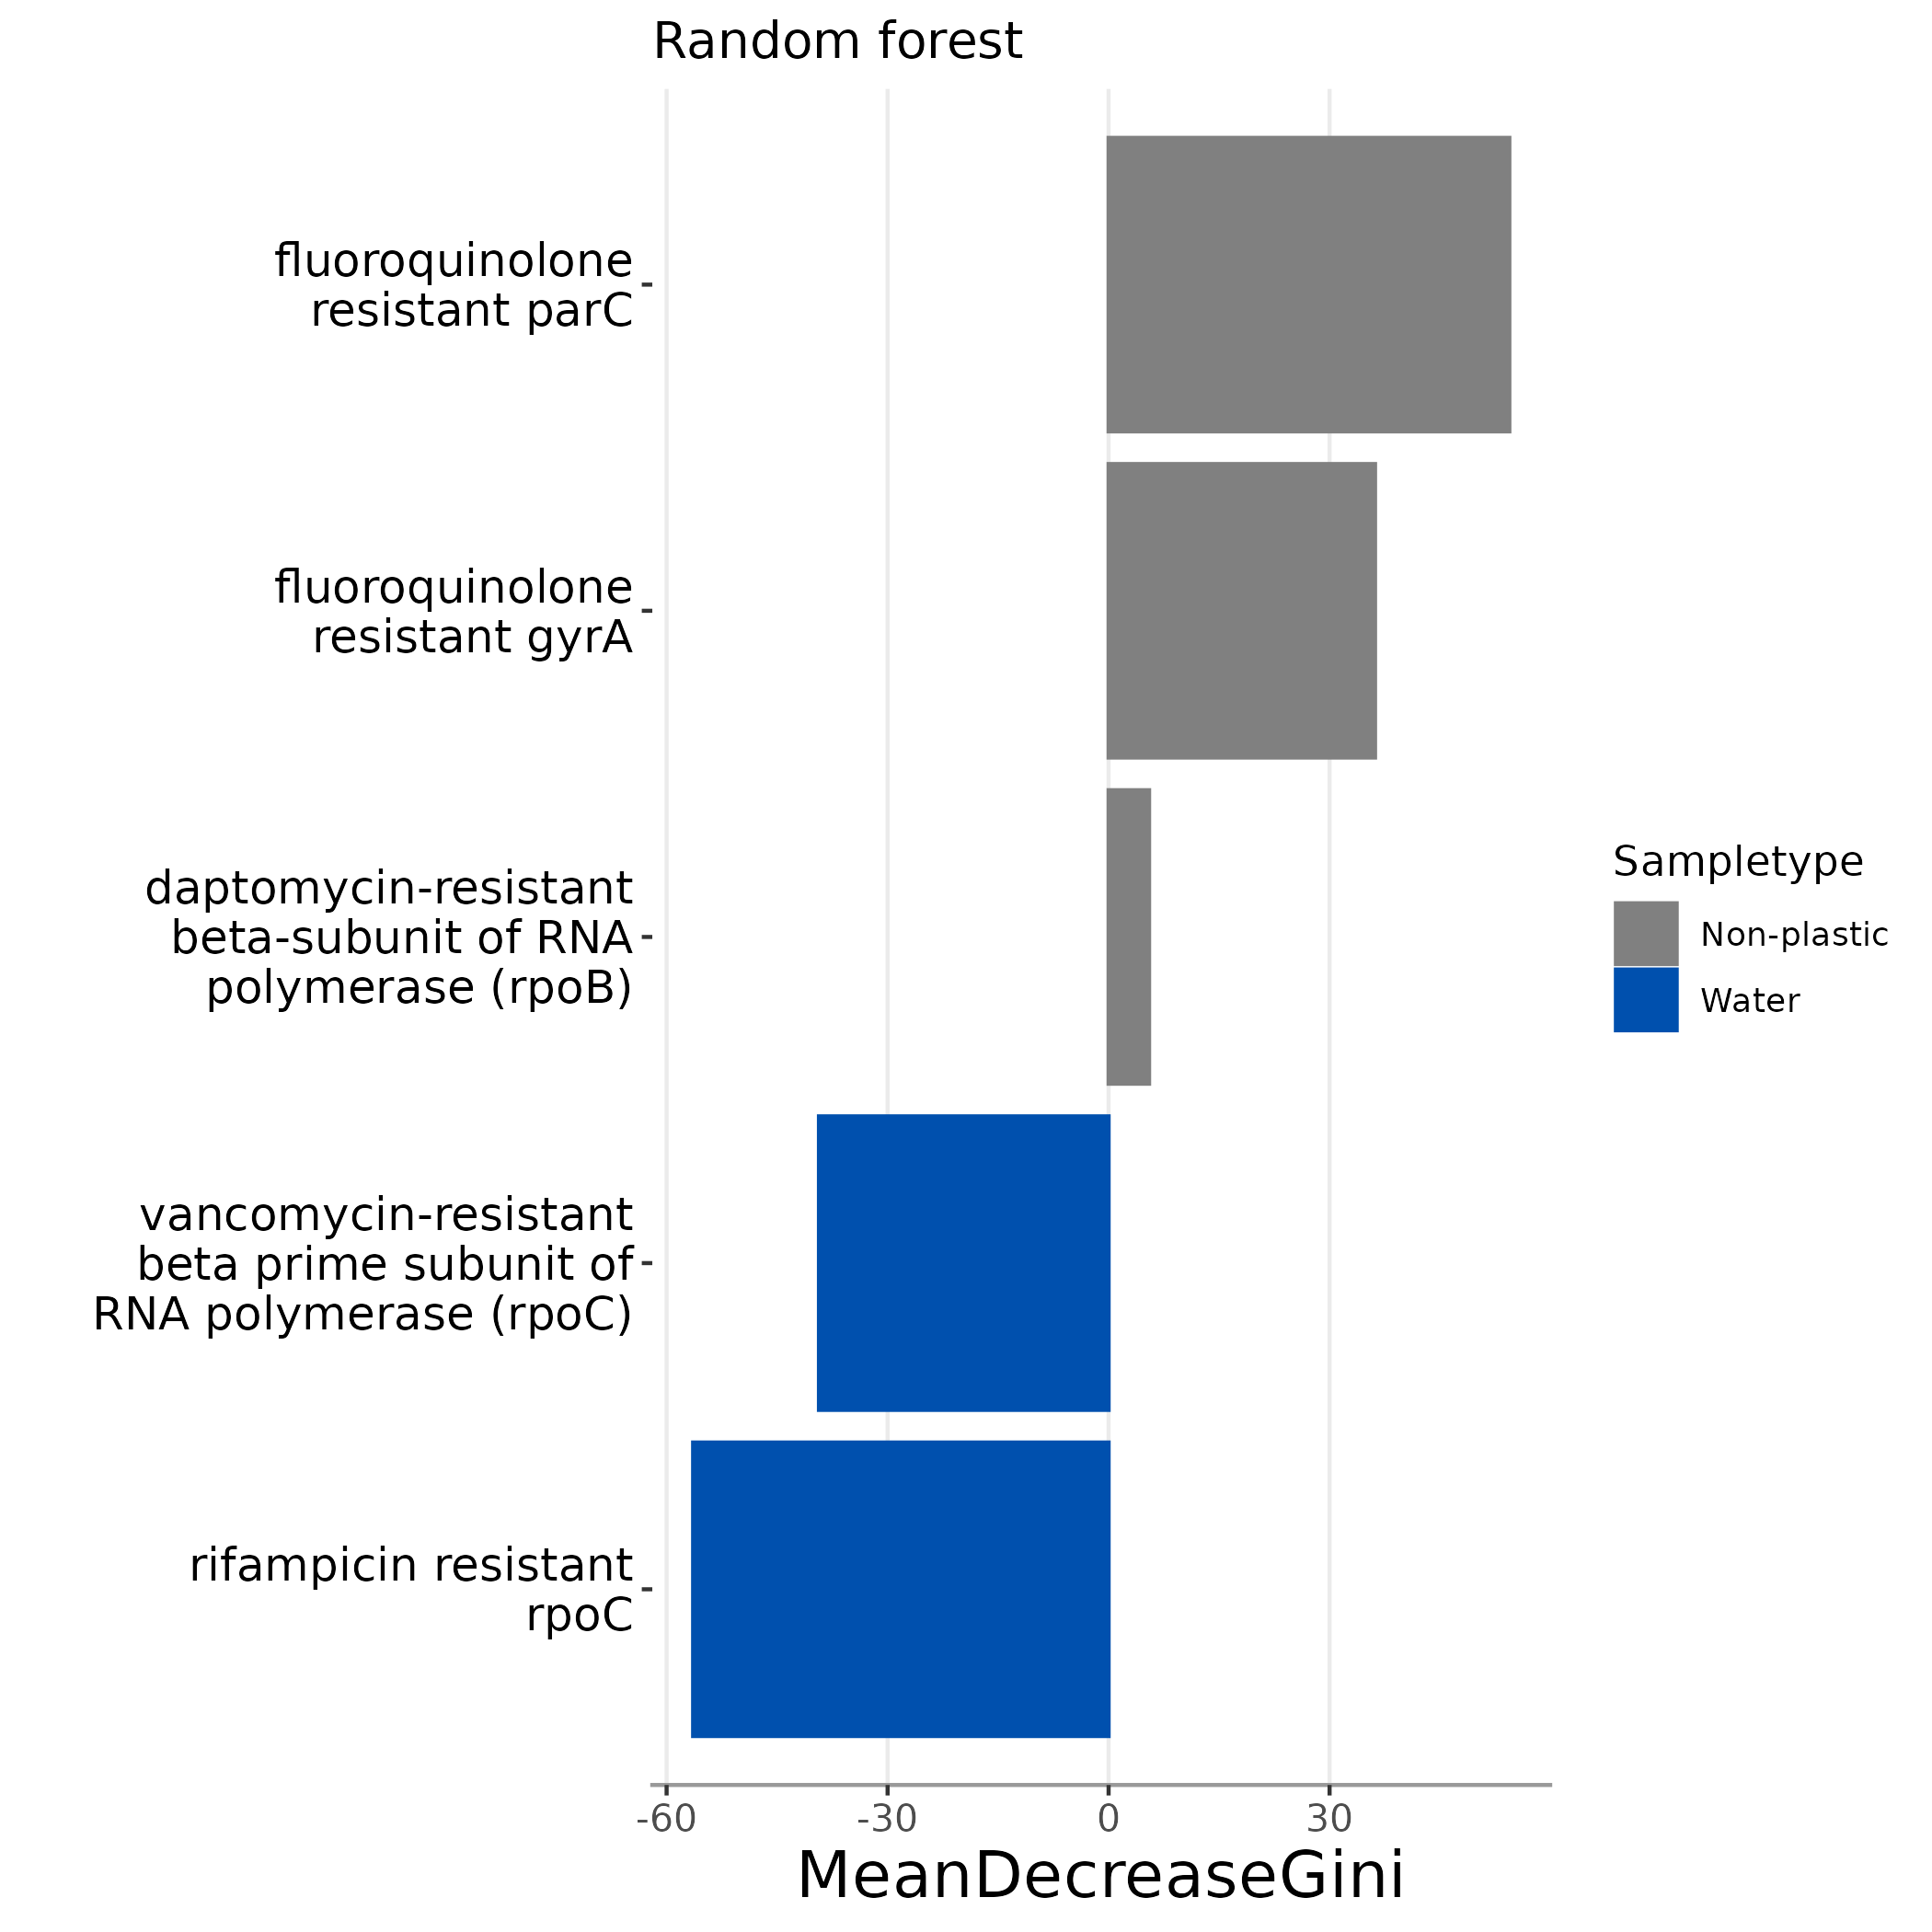
\includegraphics[width=0.5\textwidth]{figure/relative_forest_sampletype_amr_bar.png}}
    \subfloat[\label{amr_sampletype_abund}]{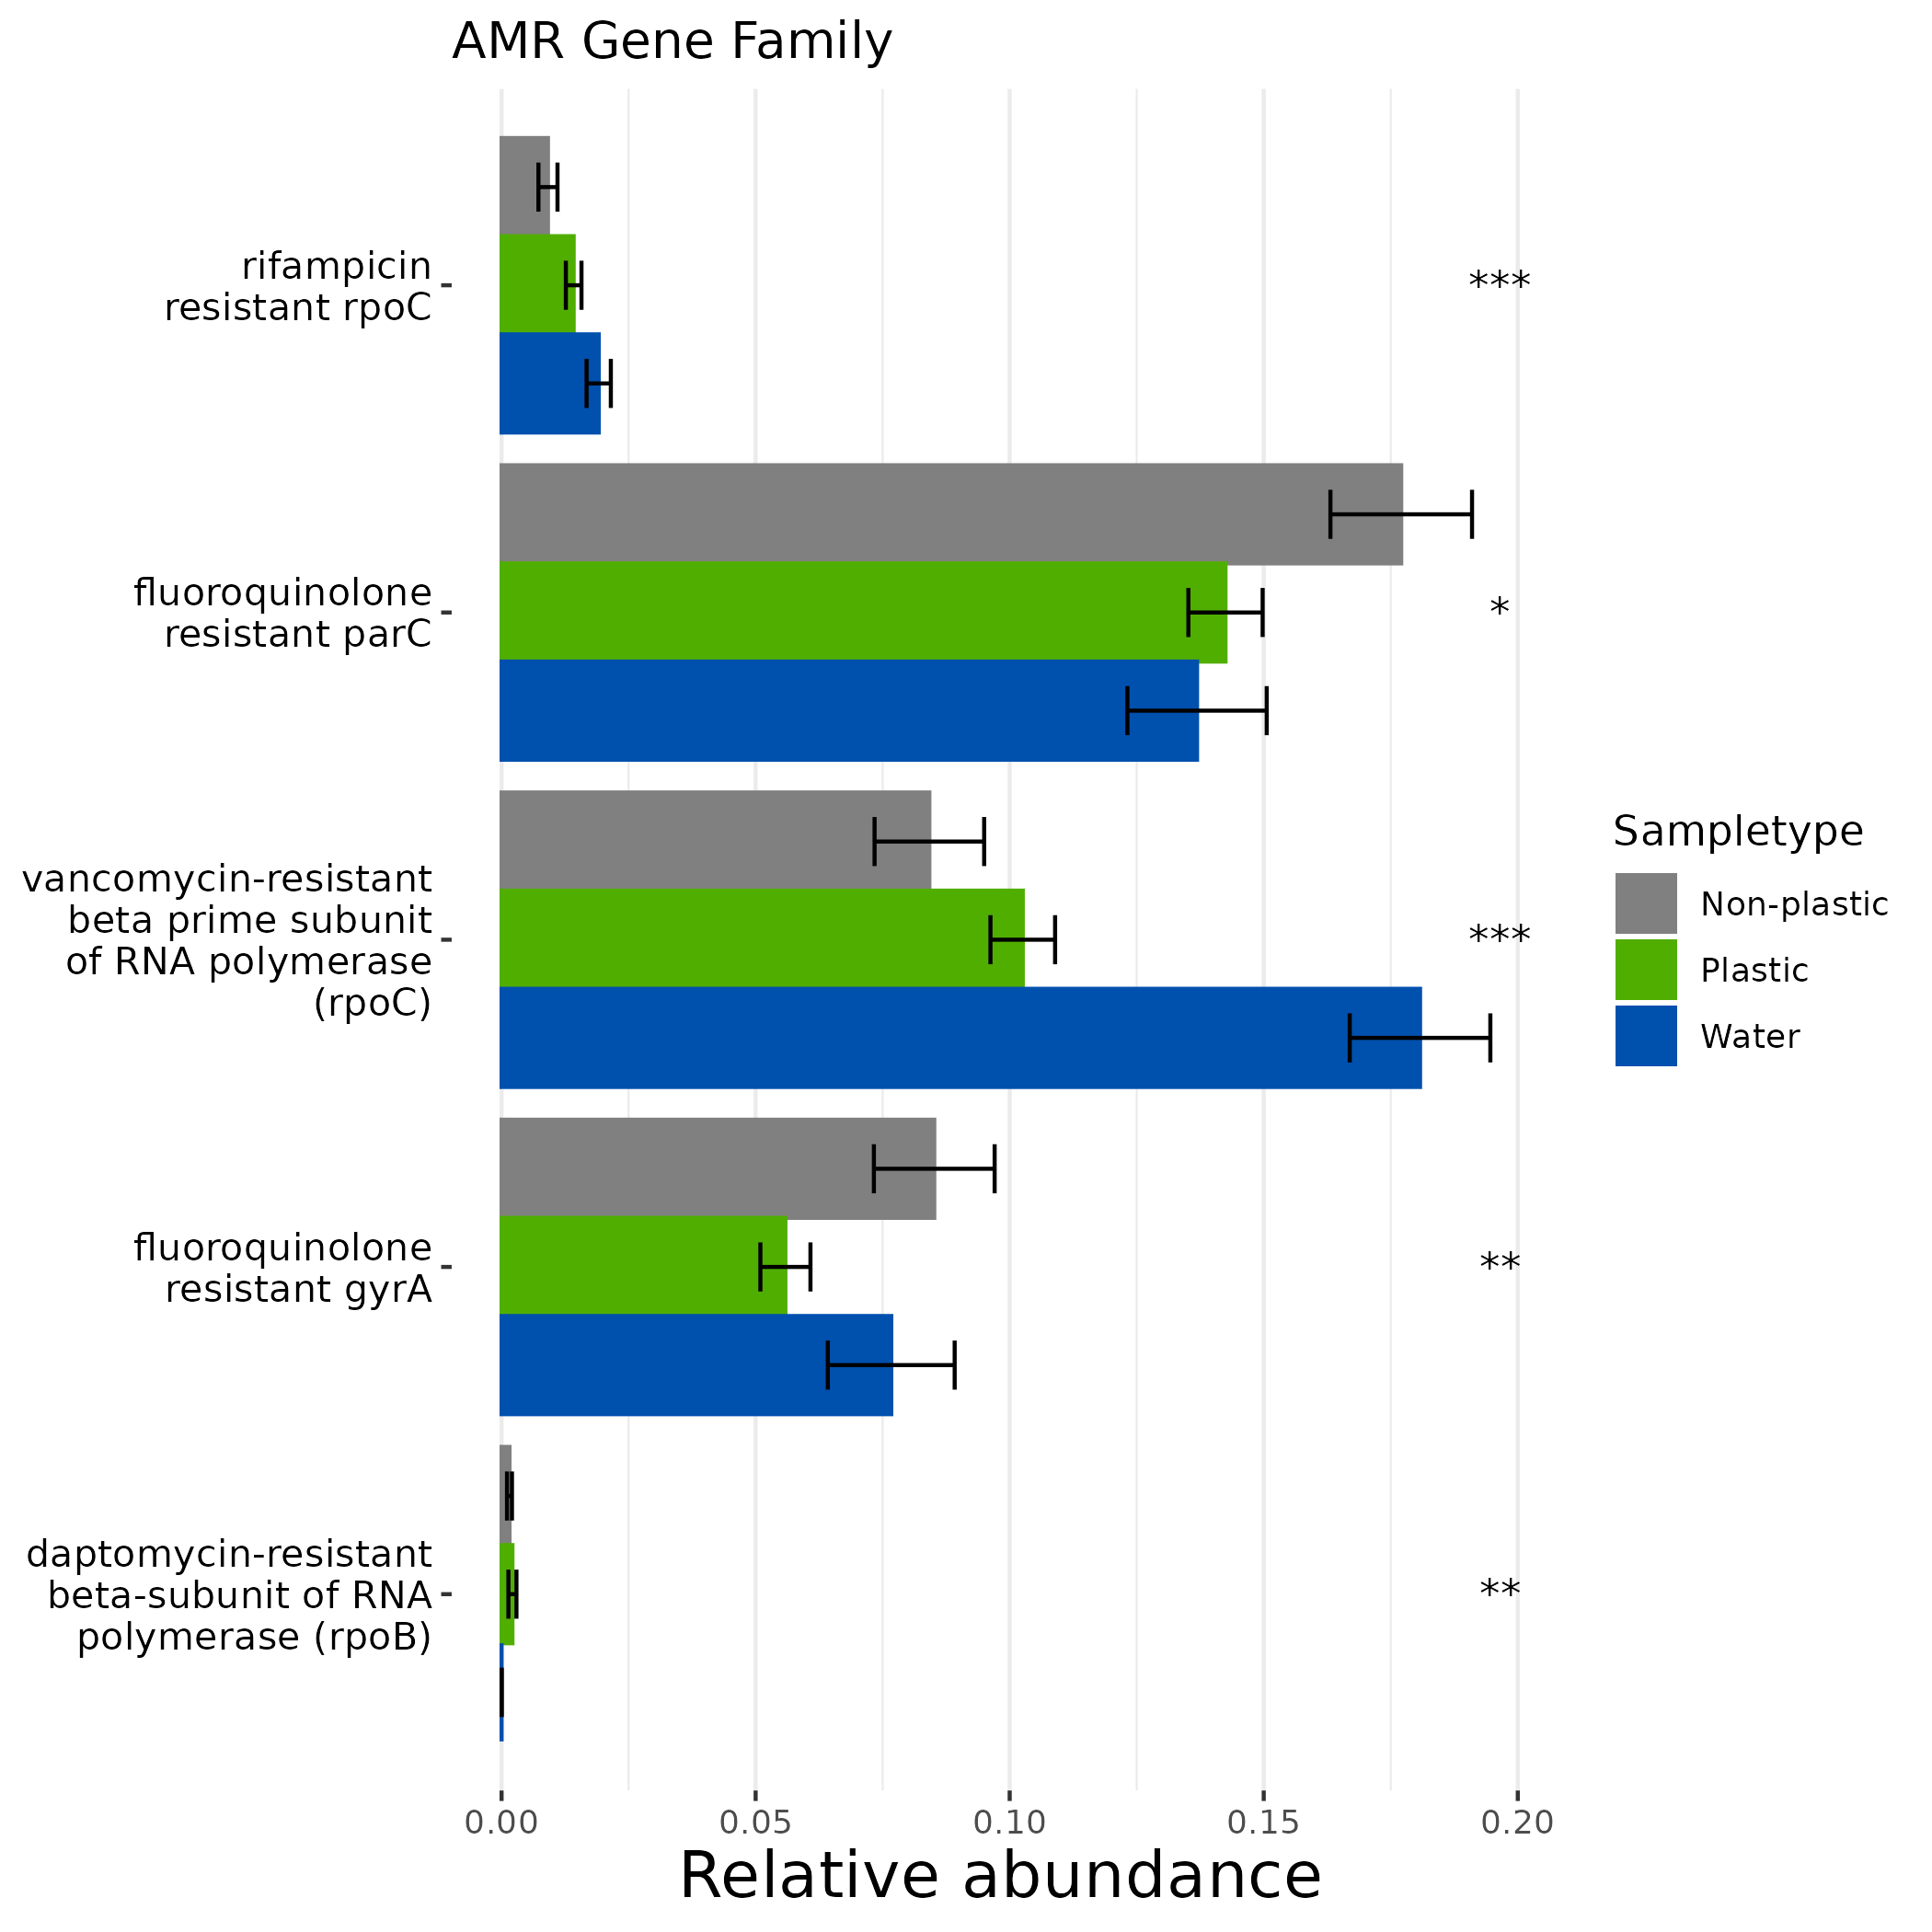
\includegraphics[width=0.5\textwidth]{figure/relative_forest_sampletype_amr_abund.png}}
    \caption{(a) Significantly assigned AMR Gene Families and Mean Decrease Gini Importance when grouped by sampletype. (b) Relative Abundances of the different AMR Gene Families in the sampletype}
    \label{amr_sampletype}
\end{figure}

If instead the samples are grouped by substrate type, as shown in figure \ref{amr_substrate_bar}, there are a lot more AMR Gene Families which distinguishes the samples in one group from another.
The most prevalent substrate in this figure is the activated sludge, which has four different AMR Gene Families that distinguishes it.
The one labelled Multiple Resistant Variants has been renamed from "ATP-binding cassette (ABC) antibiotic efflux pump; General Bacterial Porin with reduced permeability to beta-lactams; major facilitator superfamily (MFS) antibiotic efflux pump; resistance-nodulation-cell division (RND) antibiotic efflux pump". 
%\{comment or just observation?}
All Mean Decrease Gini impurity values are positive for this grouping, there are no significant AMR Gene Families which indicates that a sample is not from a specific substrate as was the case with the water sampletype. 

\begin{figure}[!h]
    \centering
    \subfloat[\label{amr_substrate_bar}]{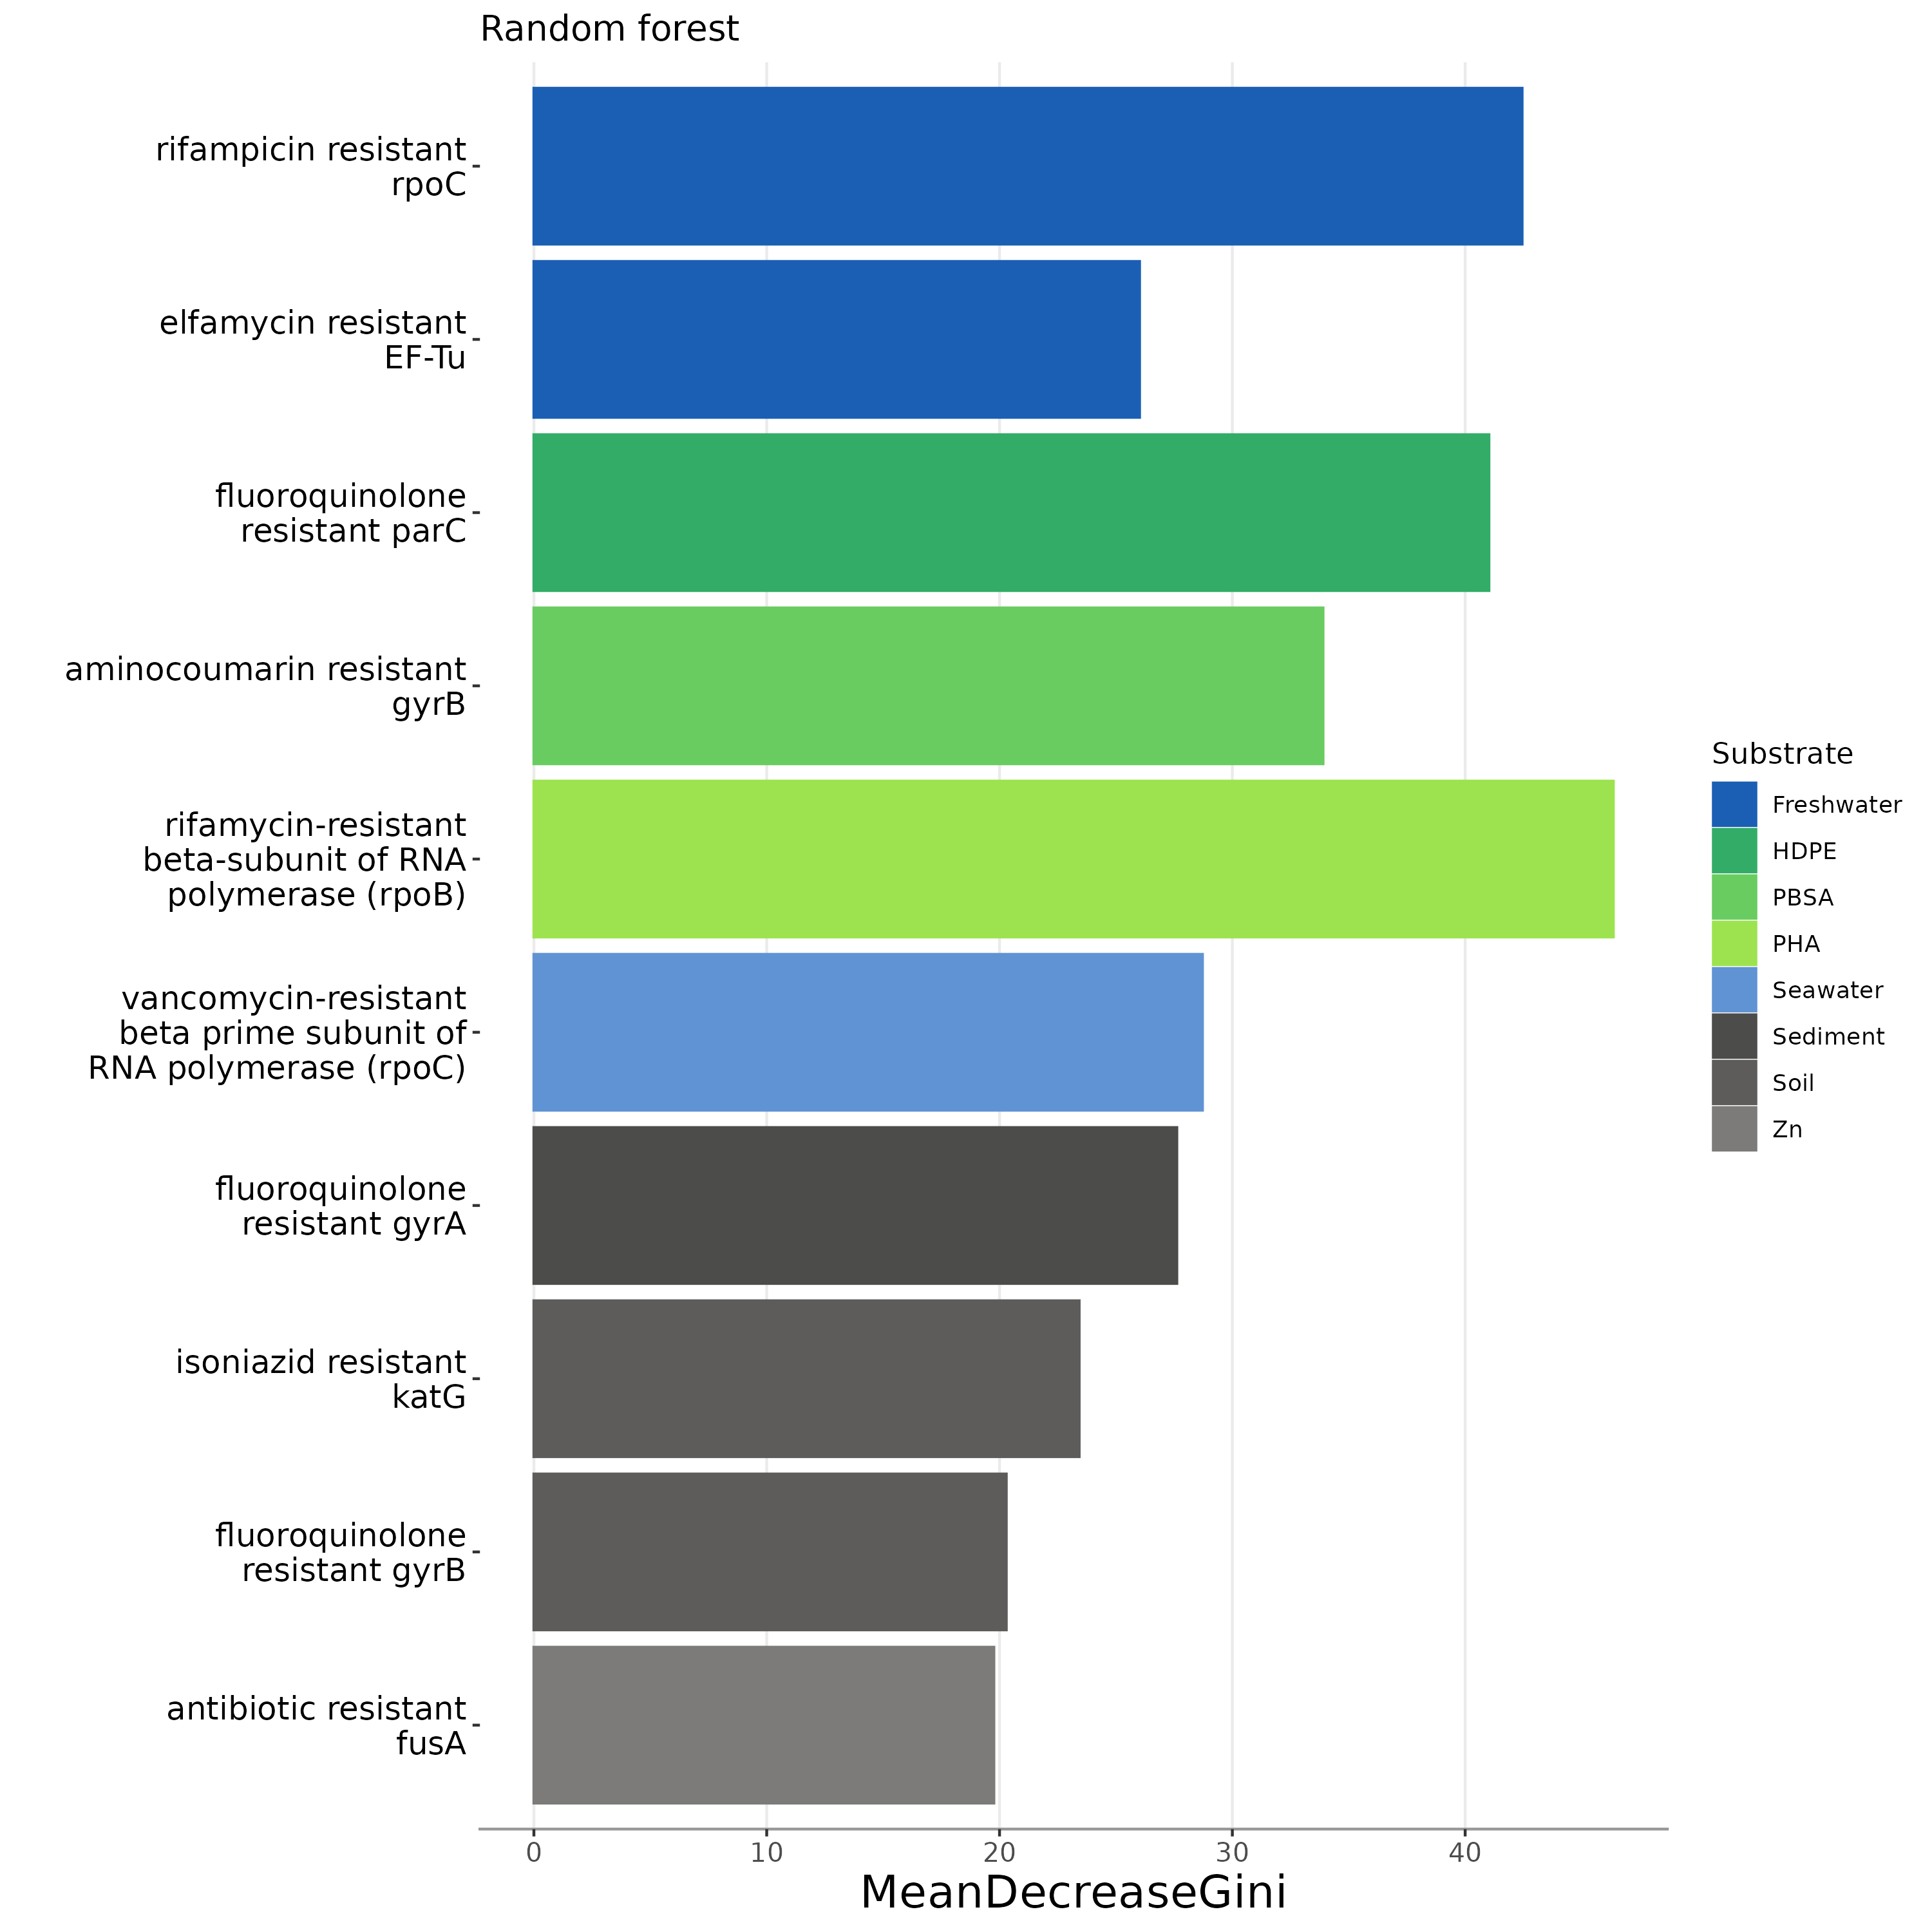
\includegraphics[width=0.5\textwidth]{figure/relative_forest_substrate_amr_bar.png}}
    \subfloat[\label{amr_substrate_abund}]{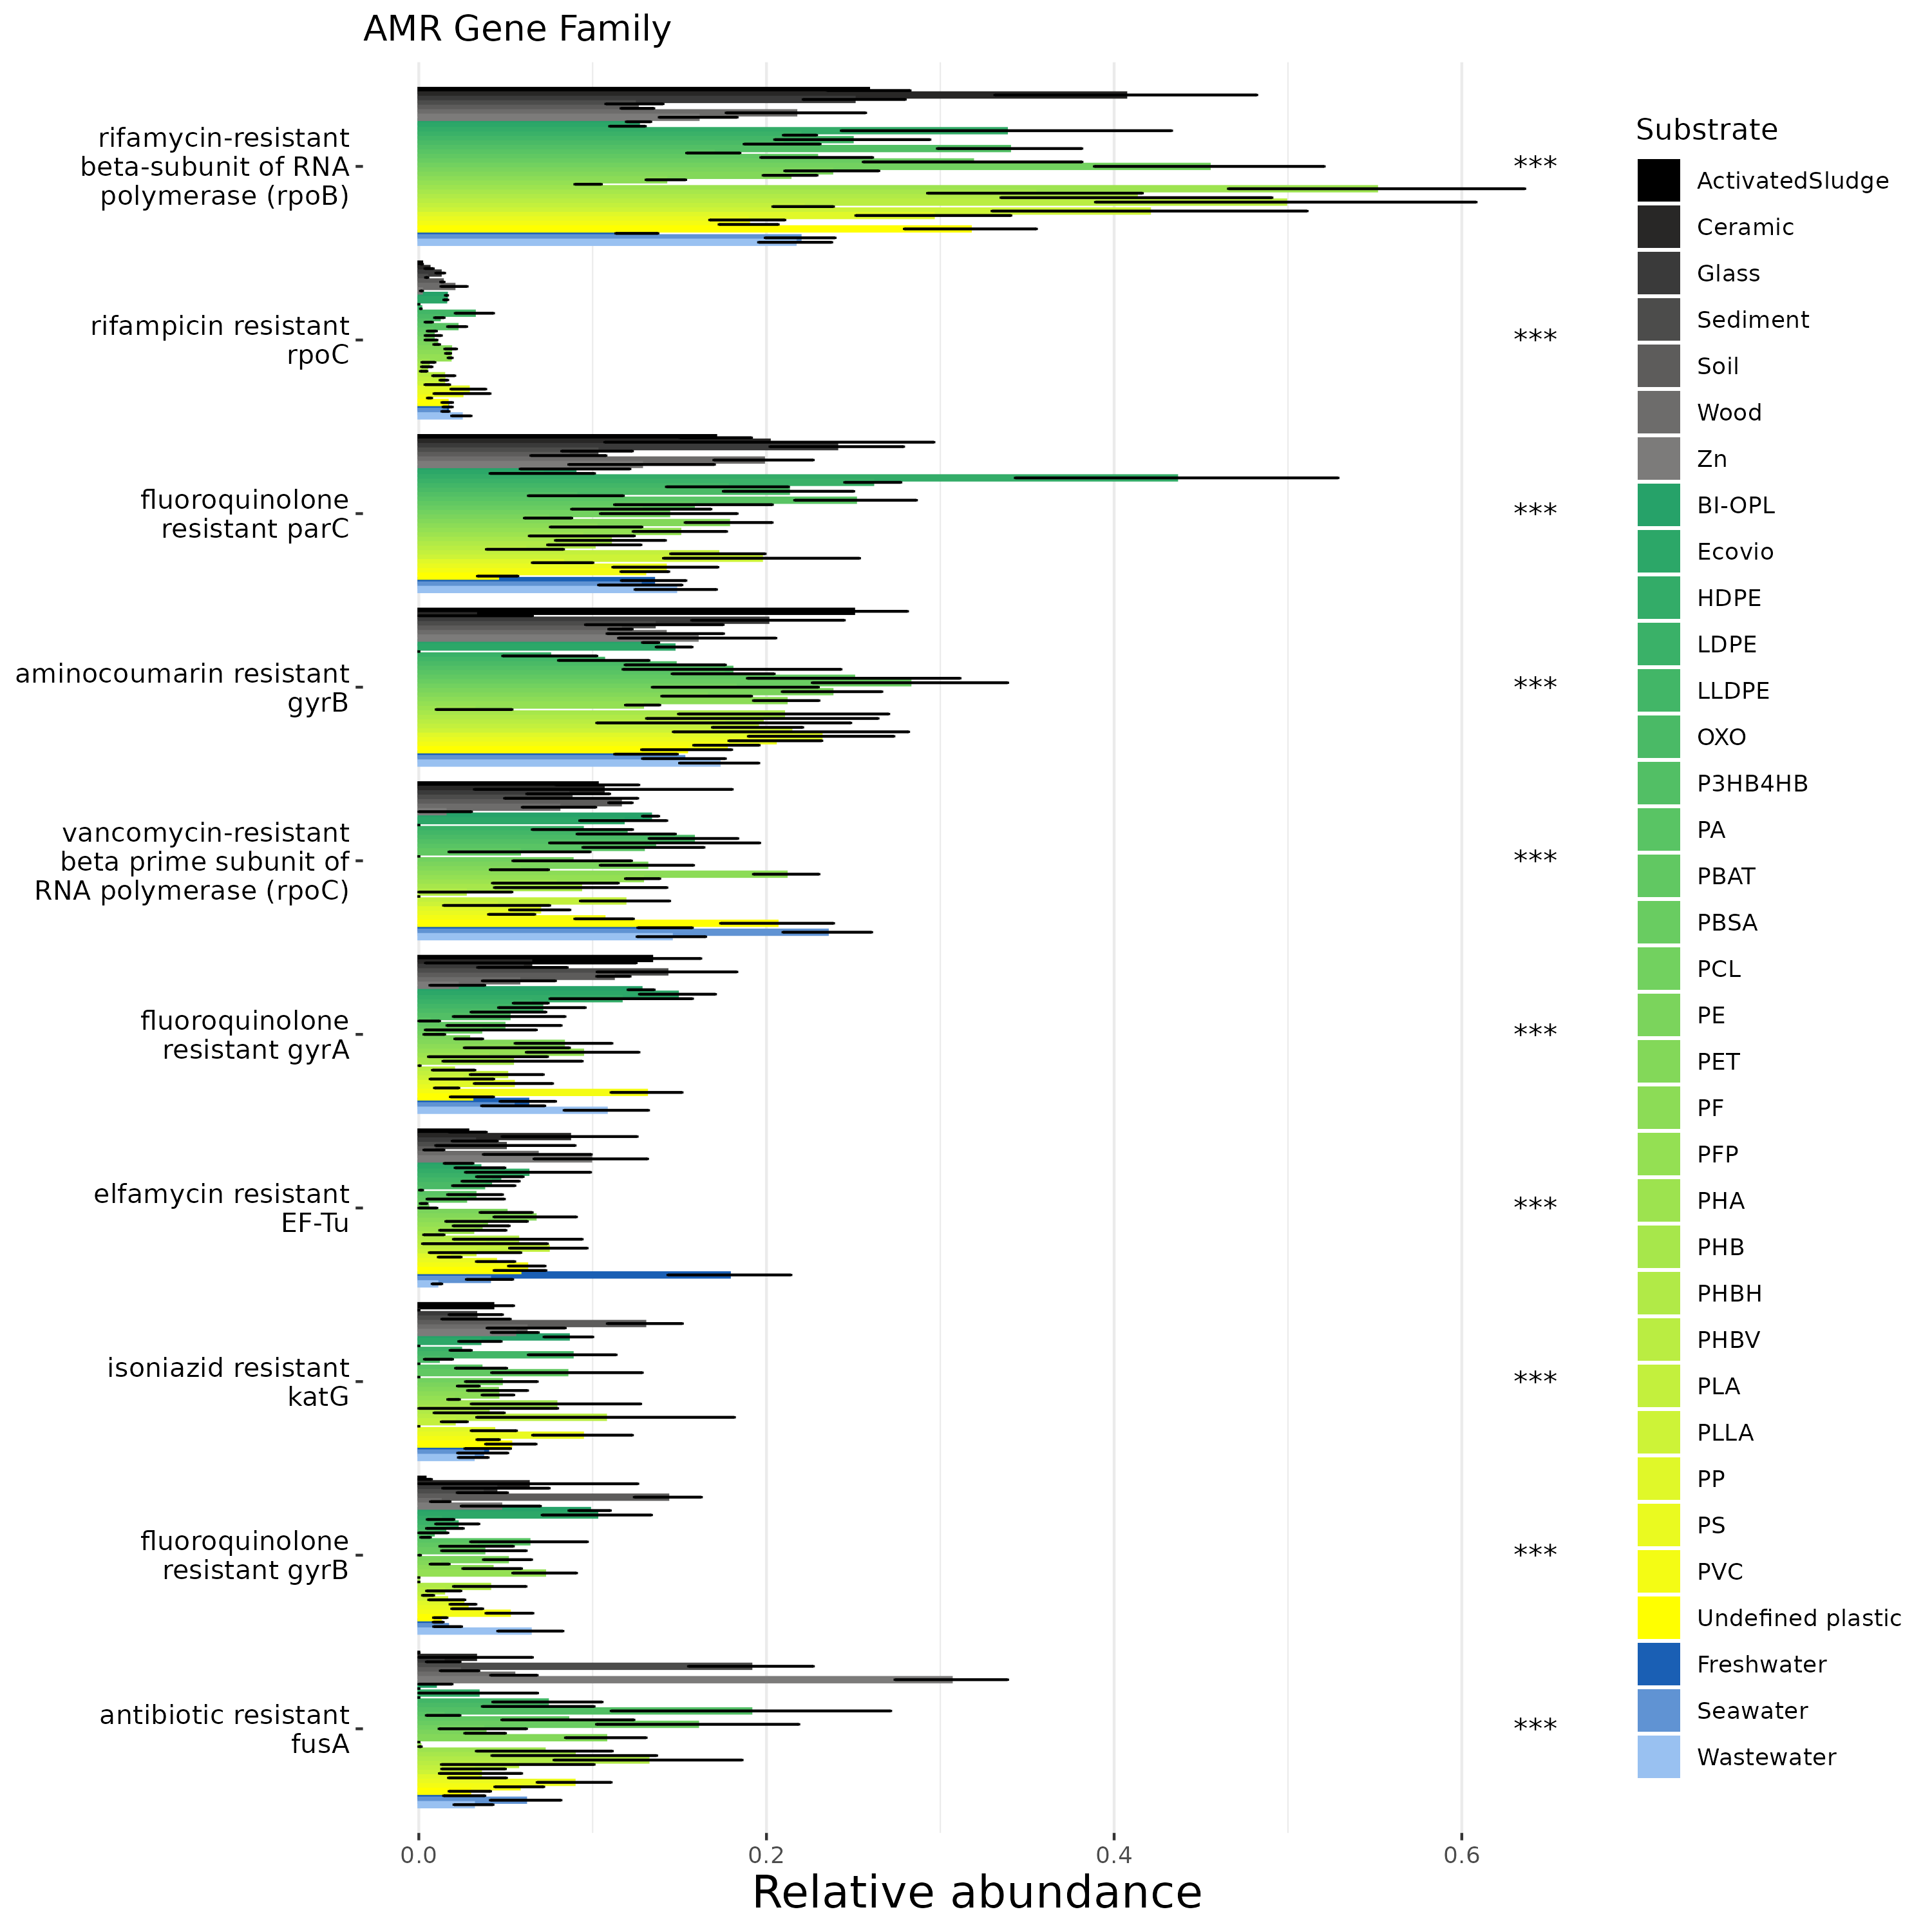
\includegraphics[width=0.5\textwidth]{figure/relative_forest_substrate_amr_abund.png}}
    \caption{(a) Significantly assigned AMR Gene Families and Mean Decrease Gini Importance when grouped by substrate. (b) Relative Abundances of the different AMR Gene Families in the substrates}
    \label{amr_substrate}
\end{figure}

\subsection{Prediciting point mutations as substrate identifiers} \todo{Predicting identity using point mutation} \todo{Substrate prediction using point mutations} \todo{Prediciting substrate identifiers using point mutations}
The following figures use the individual point mutations, or combinations thereof, found in the samples as the grouping for which the random forest analysis was performed, instead of the AMR Gene Family. 
Only the non-plastic sampletype can be significantly assigned (p < 0.05) to any mutation in figure \ref{snps_sampletype}, which includes several mutations in rpoB which confer resistance to rifampicin, as well as several in gyrA and parC which confer resistance to fluoroquinolones. 
As for the assignment to the AMR Gene Families, the water sampletype cannot be assigned to any specific point mutations directly. However one can assign a greater importance to the reference group, which consists of the two other sampletypes, than the water group for two mutations which both occur in rpoC.

%Figure \ref{snp_sampletype_bar} show the result of the analysis using the three different sampletypes as grouping, and as above only the non-plastic group and the water group are present. 
%The significant mutations for the non-plastic group include several mutations in rpoB which confer resistance to rifampicin, as well as several in gyrA and parC which confer resistance to fluoroquinolones.
%There is one combination of four mutations in rpoB which confer resistance to rifampicin. 
%However, the abundance of these mutations is relatively low, as is shown in figure \ref{snp_sampletype_abund}.

\begin{figure}[h]
    \centering
    \subfloat[\label{snp_sampletype_bar}]{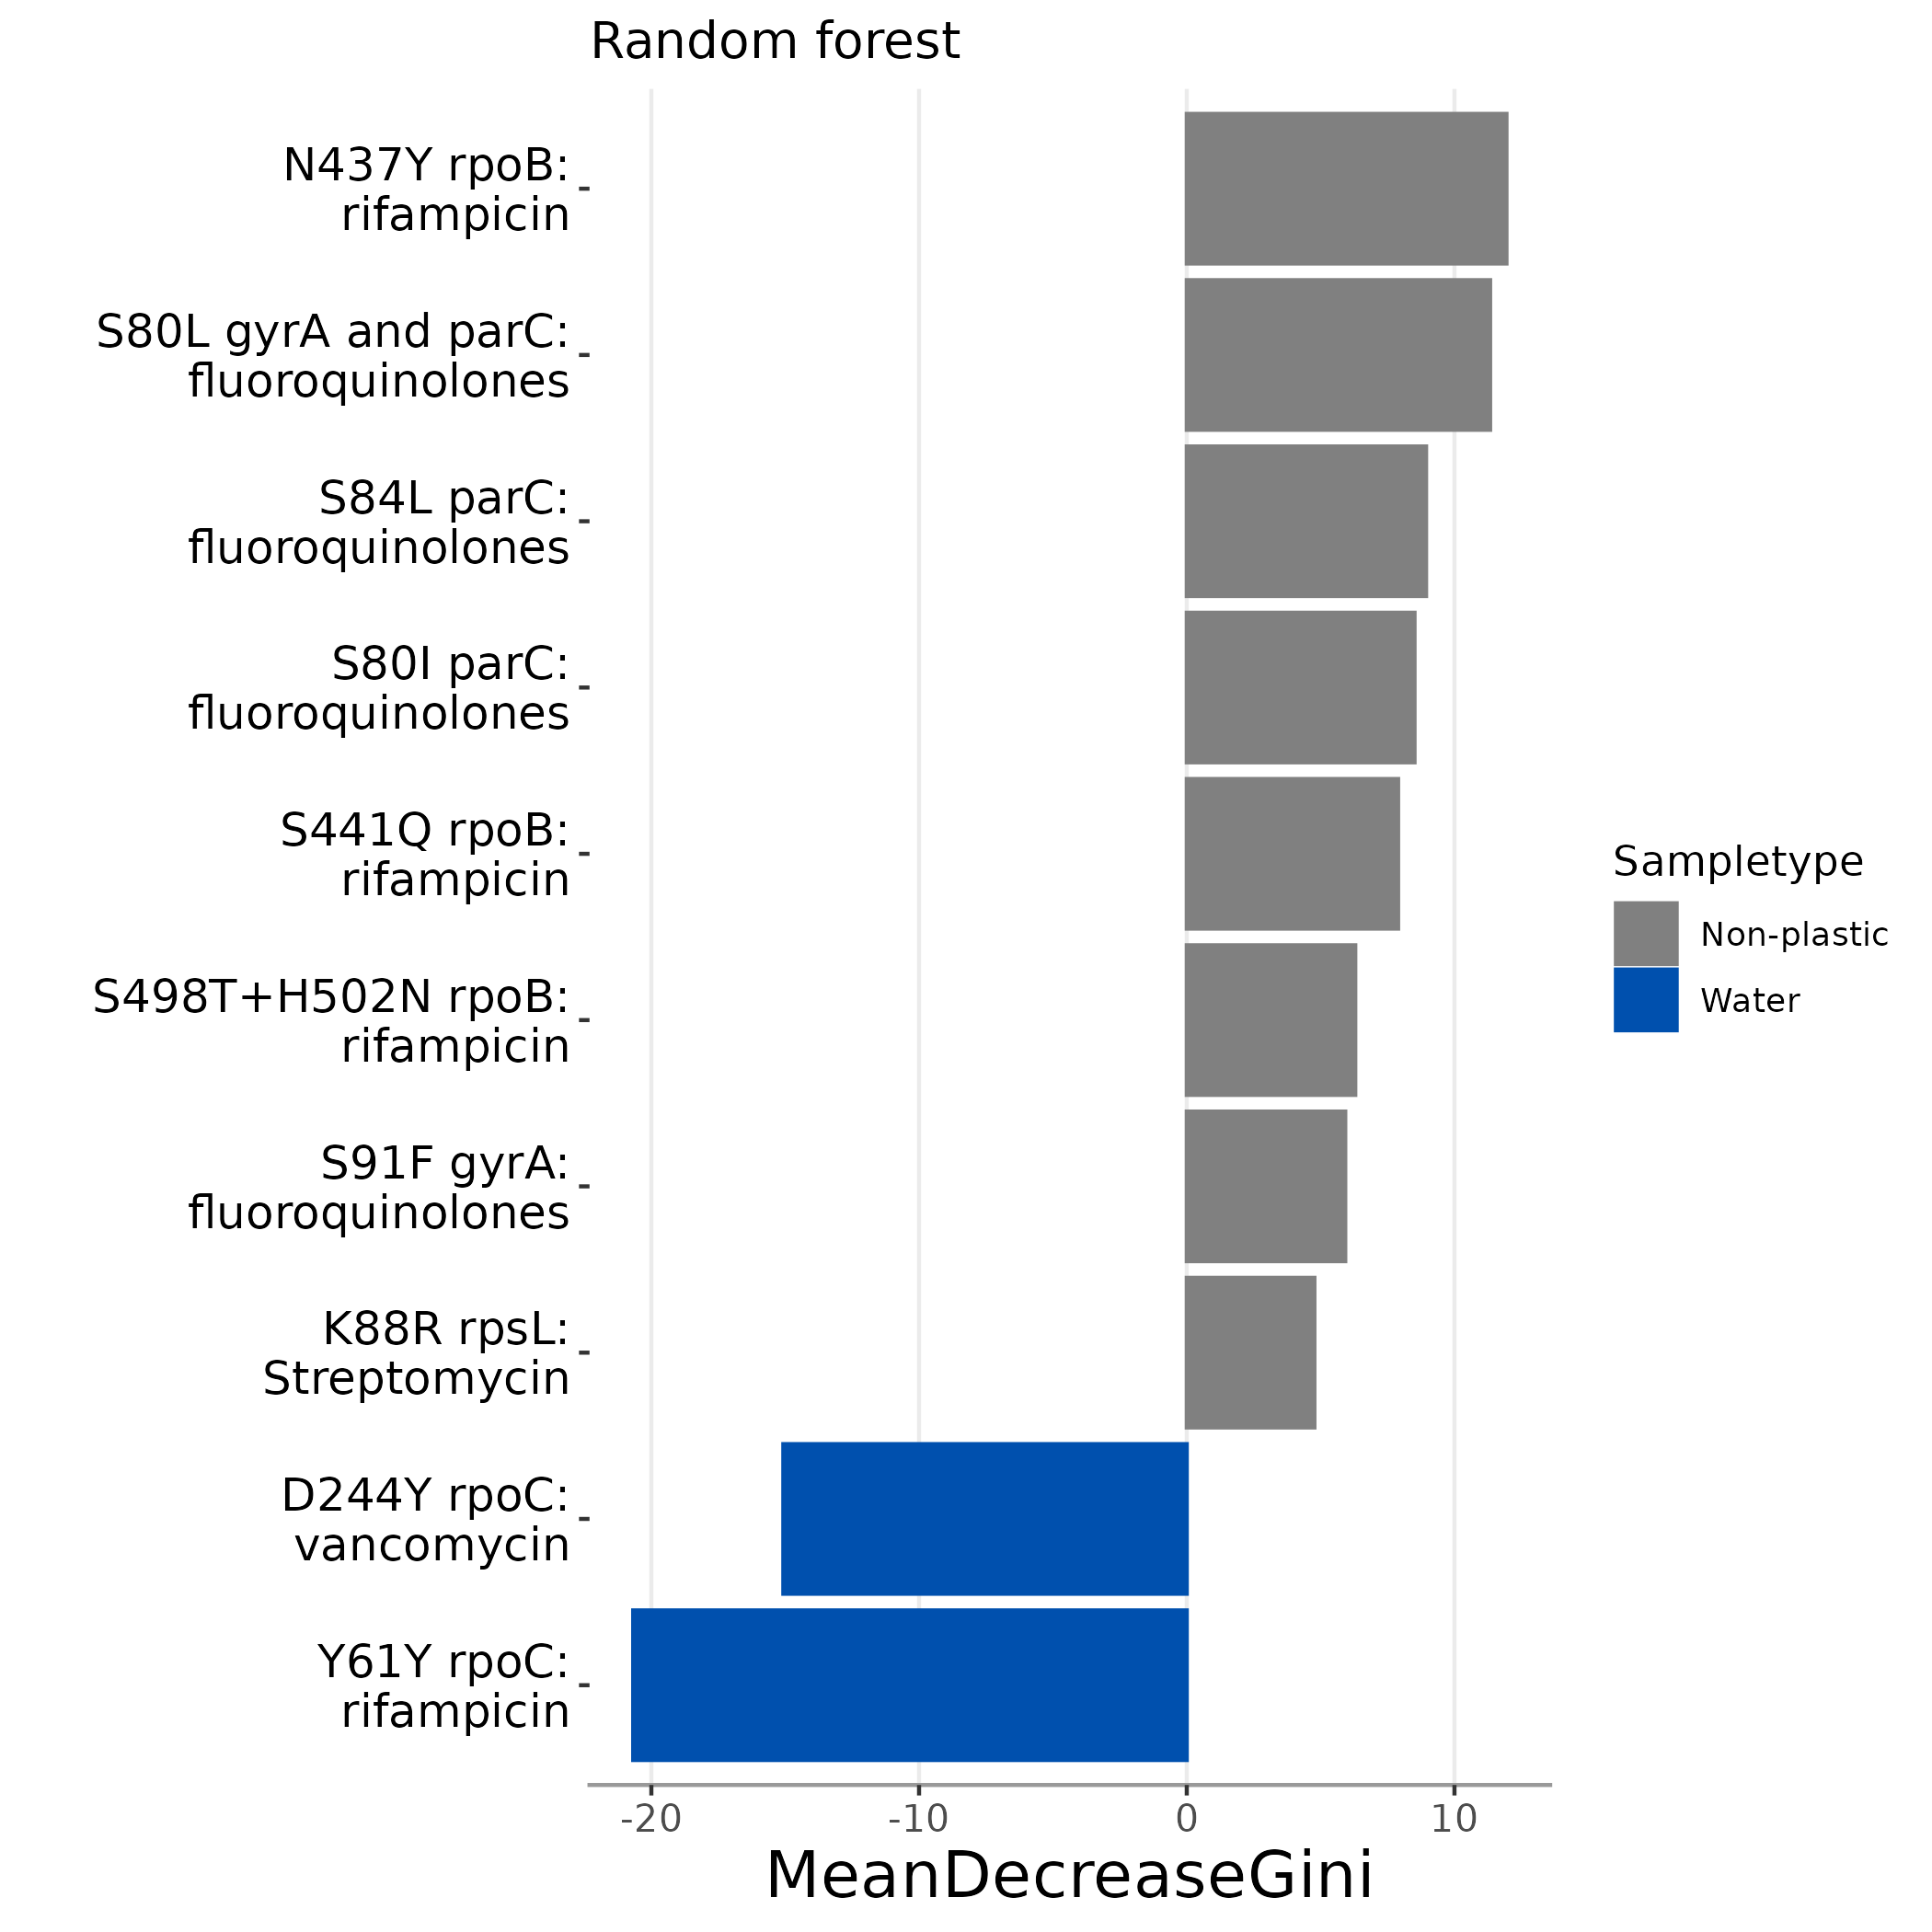
\includegraphics[width=0.5\textwidth]{figure/relative_forest_sampletype_snps_bar.png}}
    \subfloat[\label{snp_sampletype_abund}]{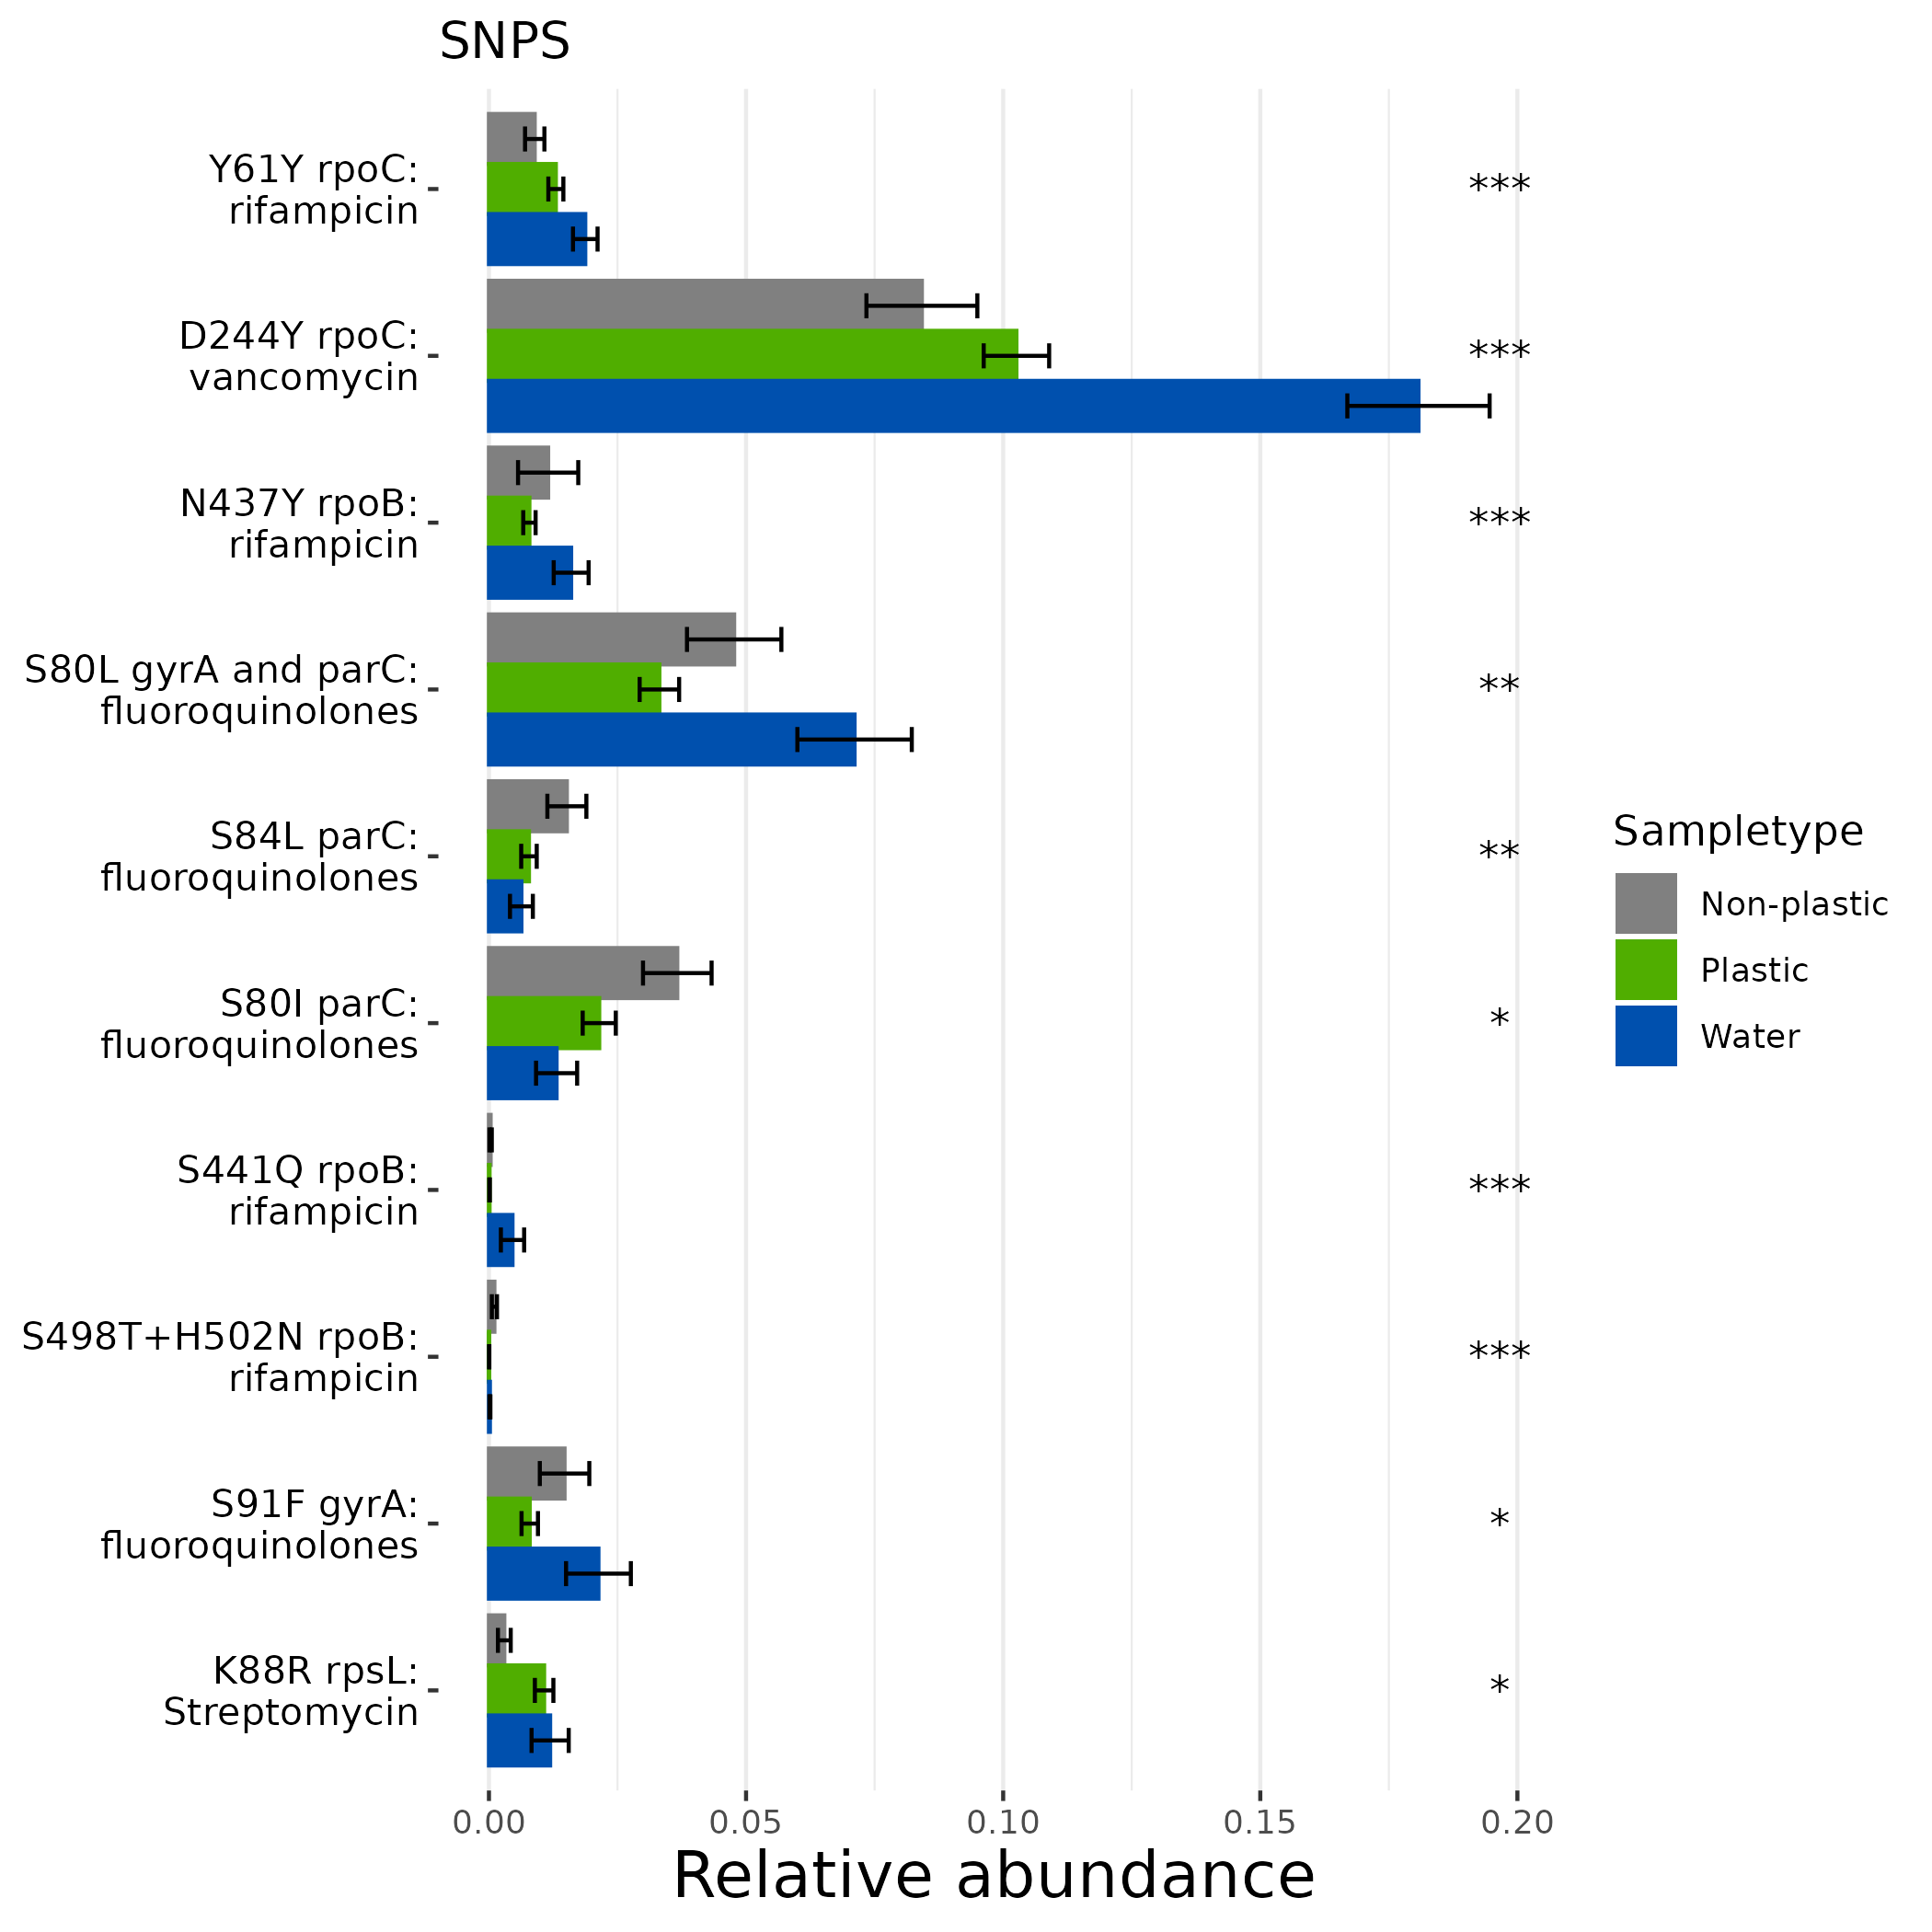
\includegraphics[width=0.5\textwidth]{figure/relative_forest_sampletype_snps_abund.png}}
    \caption{(a) Significantly assigned point mutations and Mean Decrease Gini Importance when grouped by sampletype. (b) Relative Abundances of the different point mutations in the sampletypes}
    \label{snps_sampletype}
\end{figure}

When instead the different substrates is used as the grouping variable in the random forest analysis, the mutations with the highest mean decrease Gini importance are not the same, however many of the genes and the resistances they confer are. These include parC (fluoroquinolones), rpoB (rifampicin), rpoC (rifampicin or vancomycin), gyrB (aminocoumarin), and are shown in figure \ref{snp_substrate_bar}. The mutations in EF-Tu, which confer resistance to pulvomycin, are not present in the previous plot, and may be used to identify ceramic as a substrate. Note however that there are only three ceramic samples in this study, which may skew the results.
%\{note however that there are only 3 ceramic samples used in this study, which may skew the results.}

\begin{figure}[h!]
    \centering
    \subfloat[caption1.\label{snp_substrate_bar}]{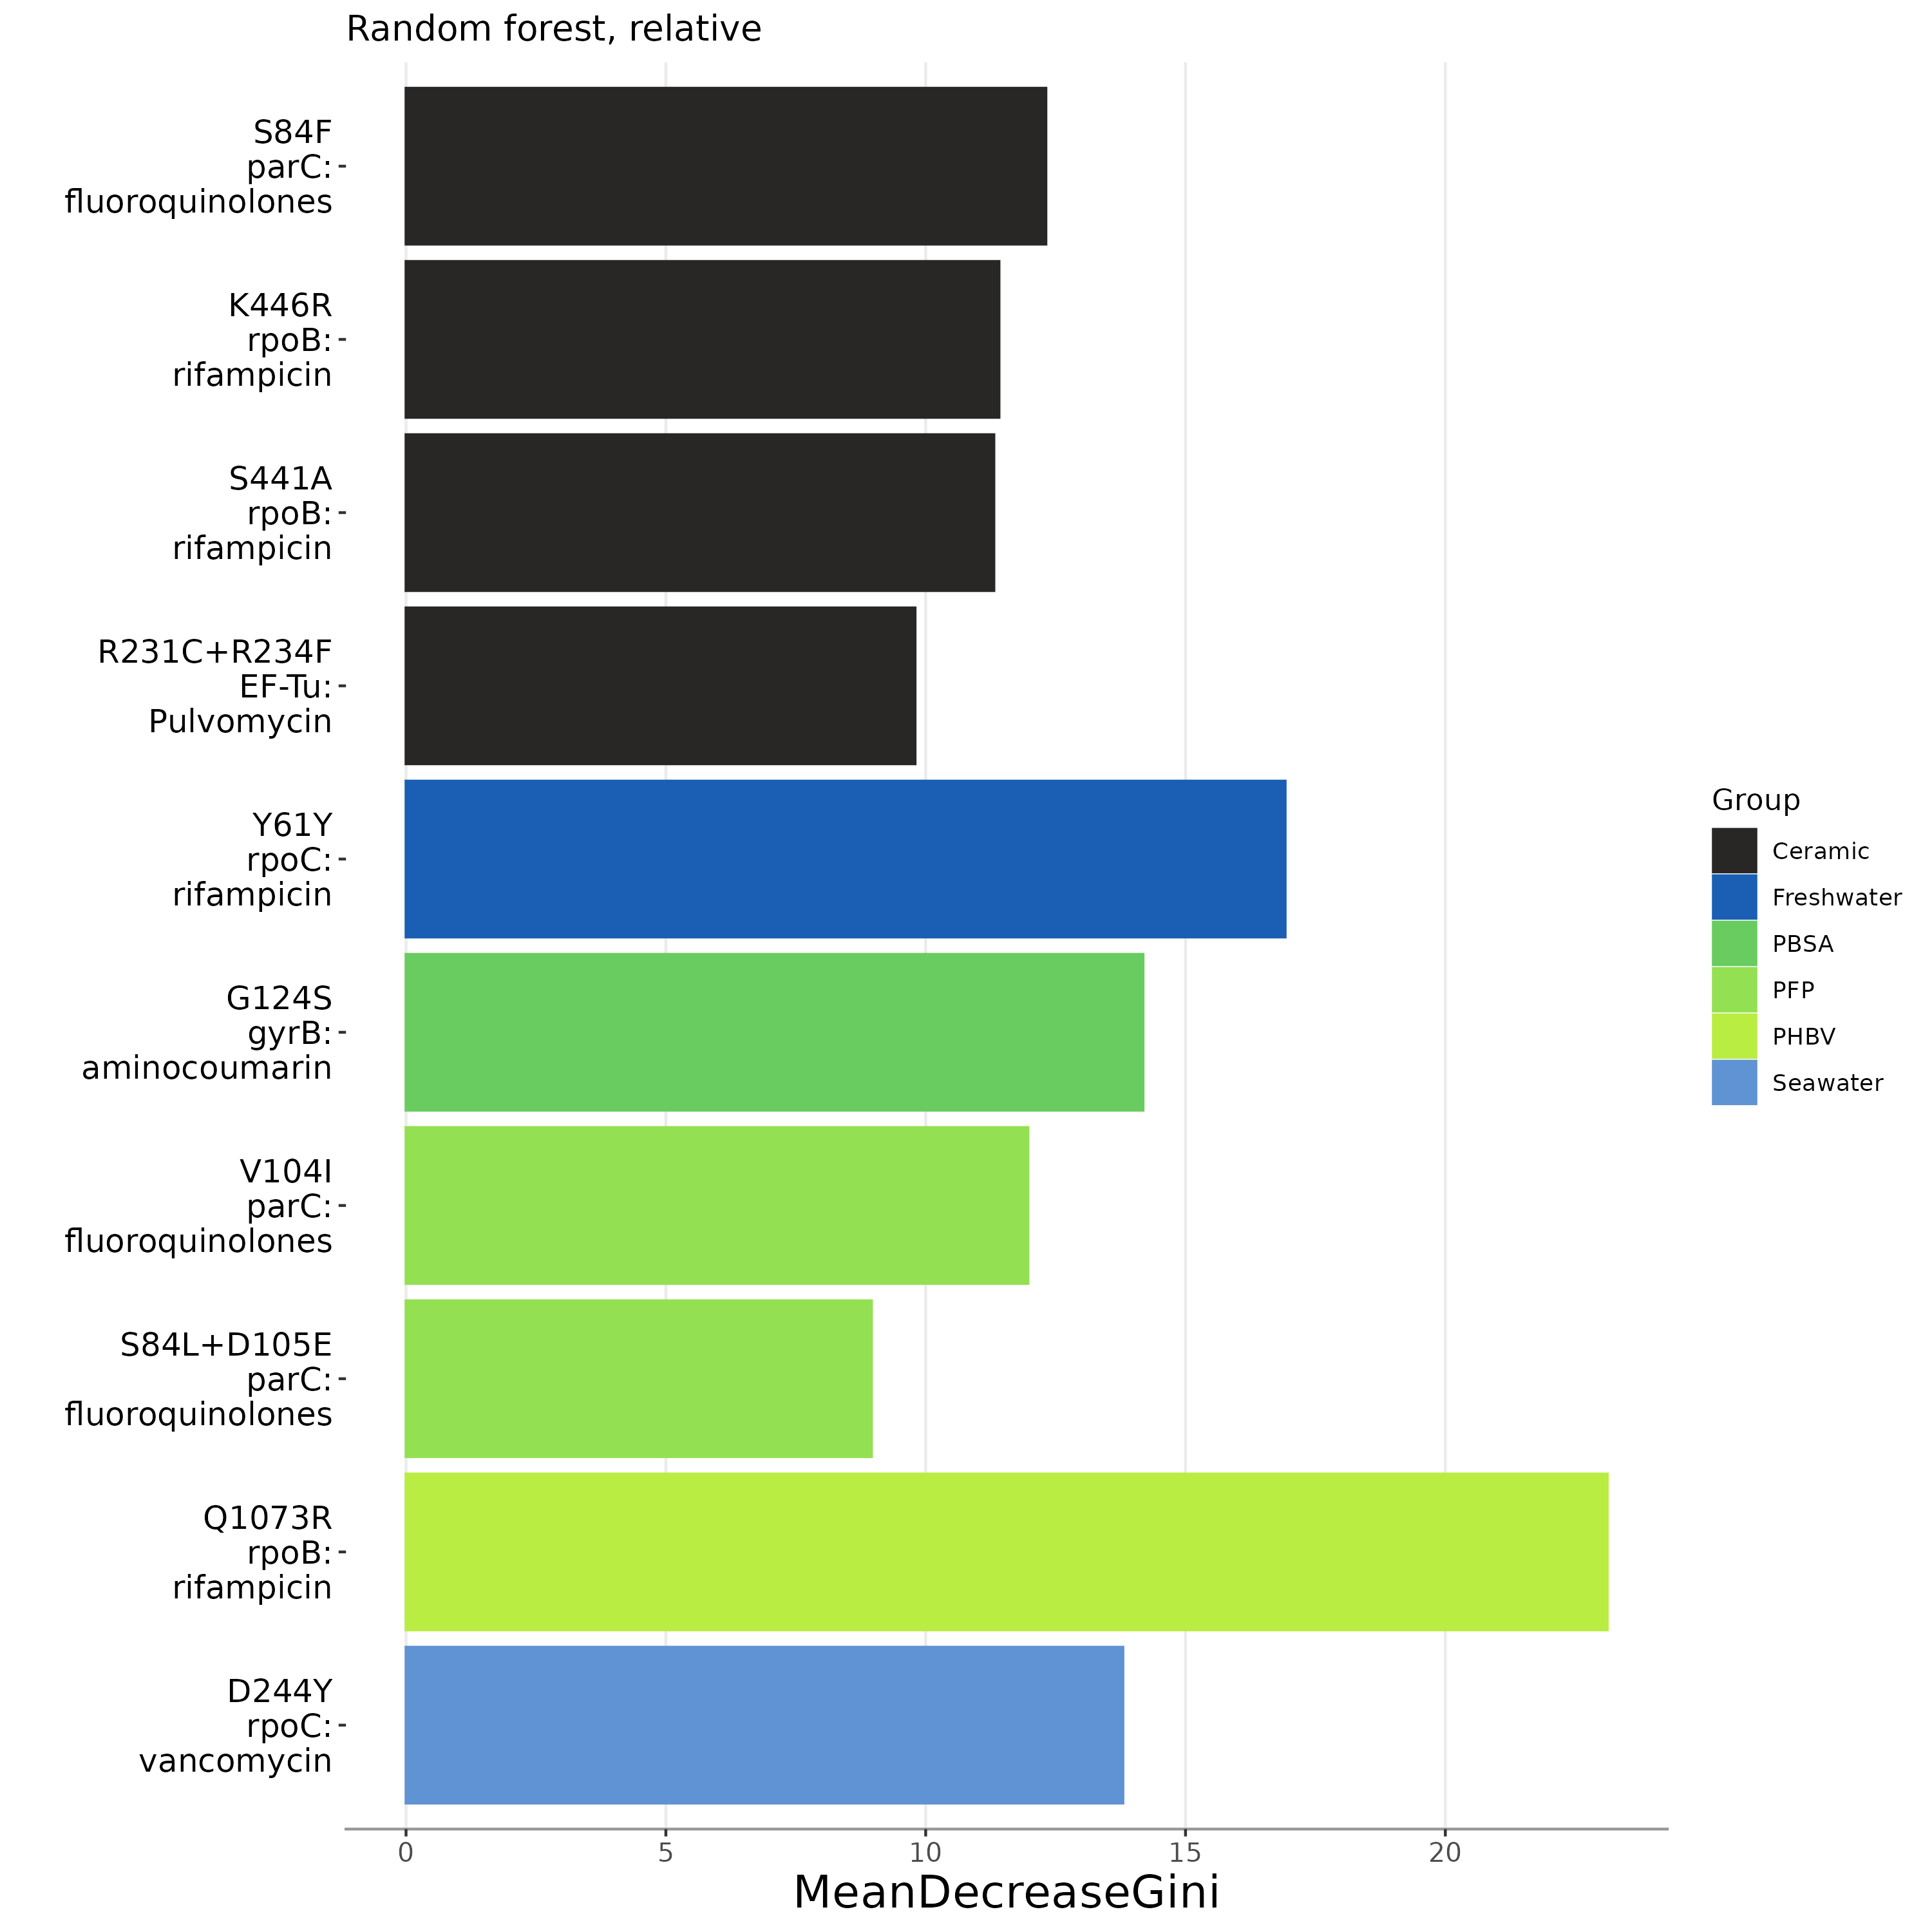
\includegraphics[width=0.5\textwidth]{figure/relative_forest_substrate_snps_bar.png}}
    \subfloat[caption2.\label{snp_substrate_abund}]{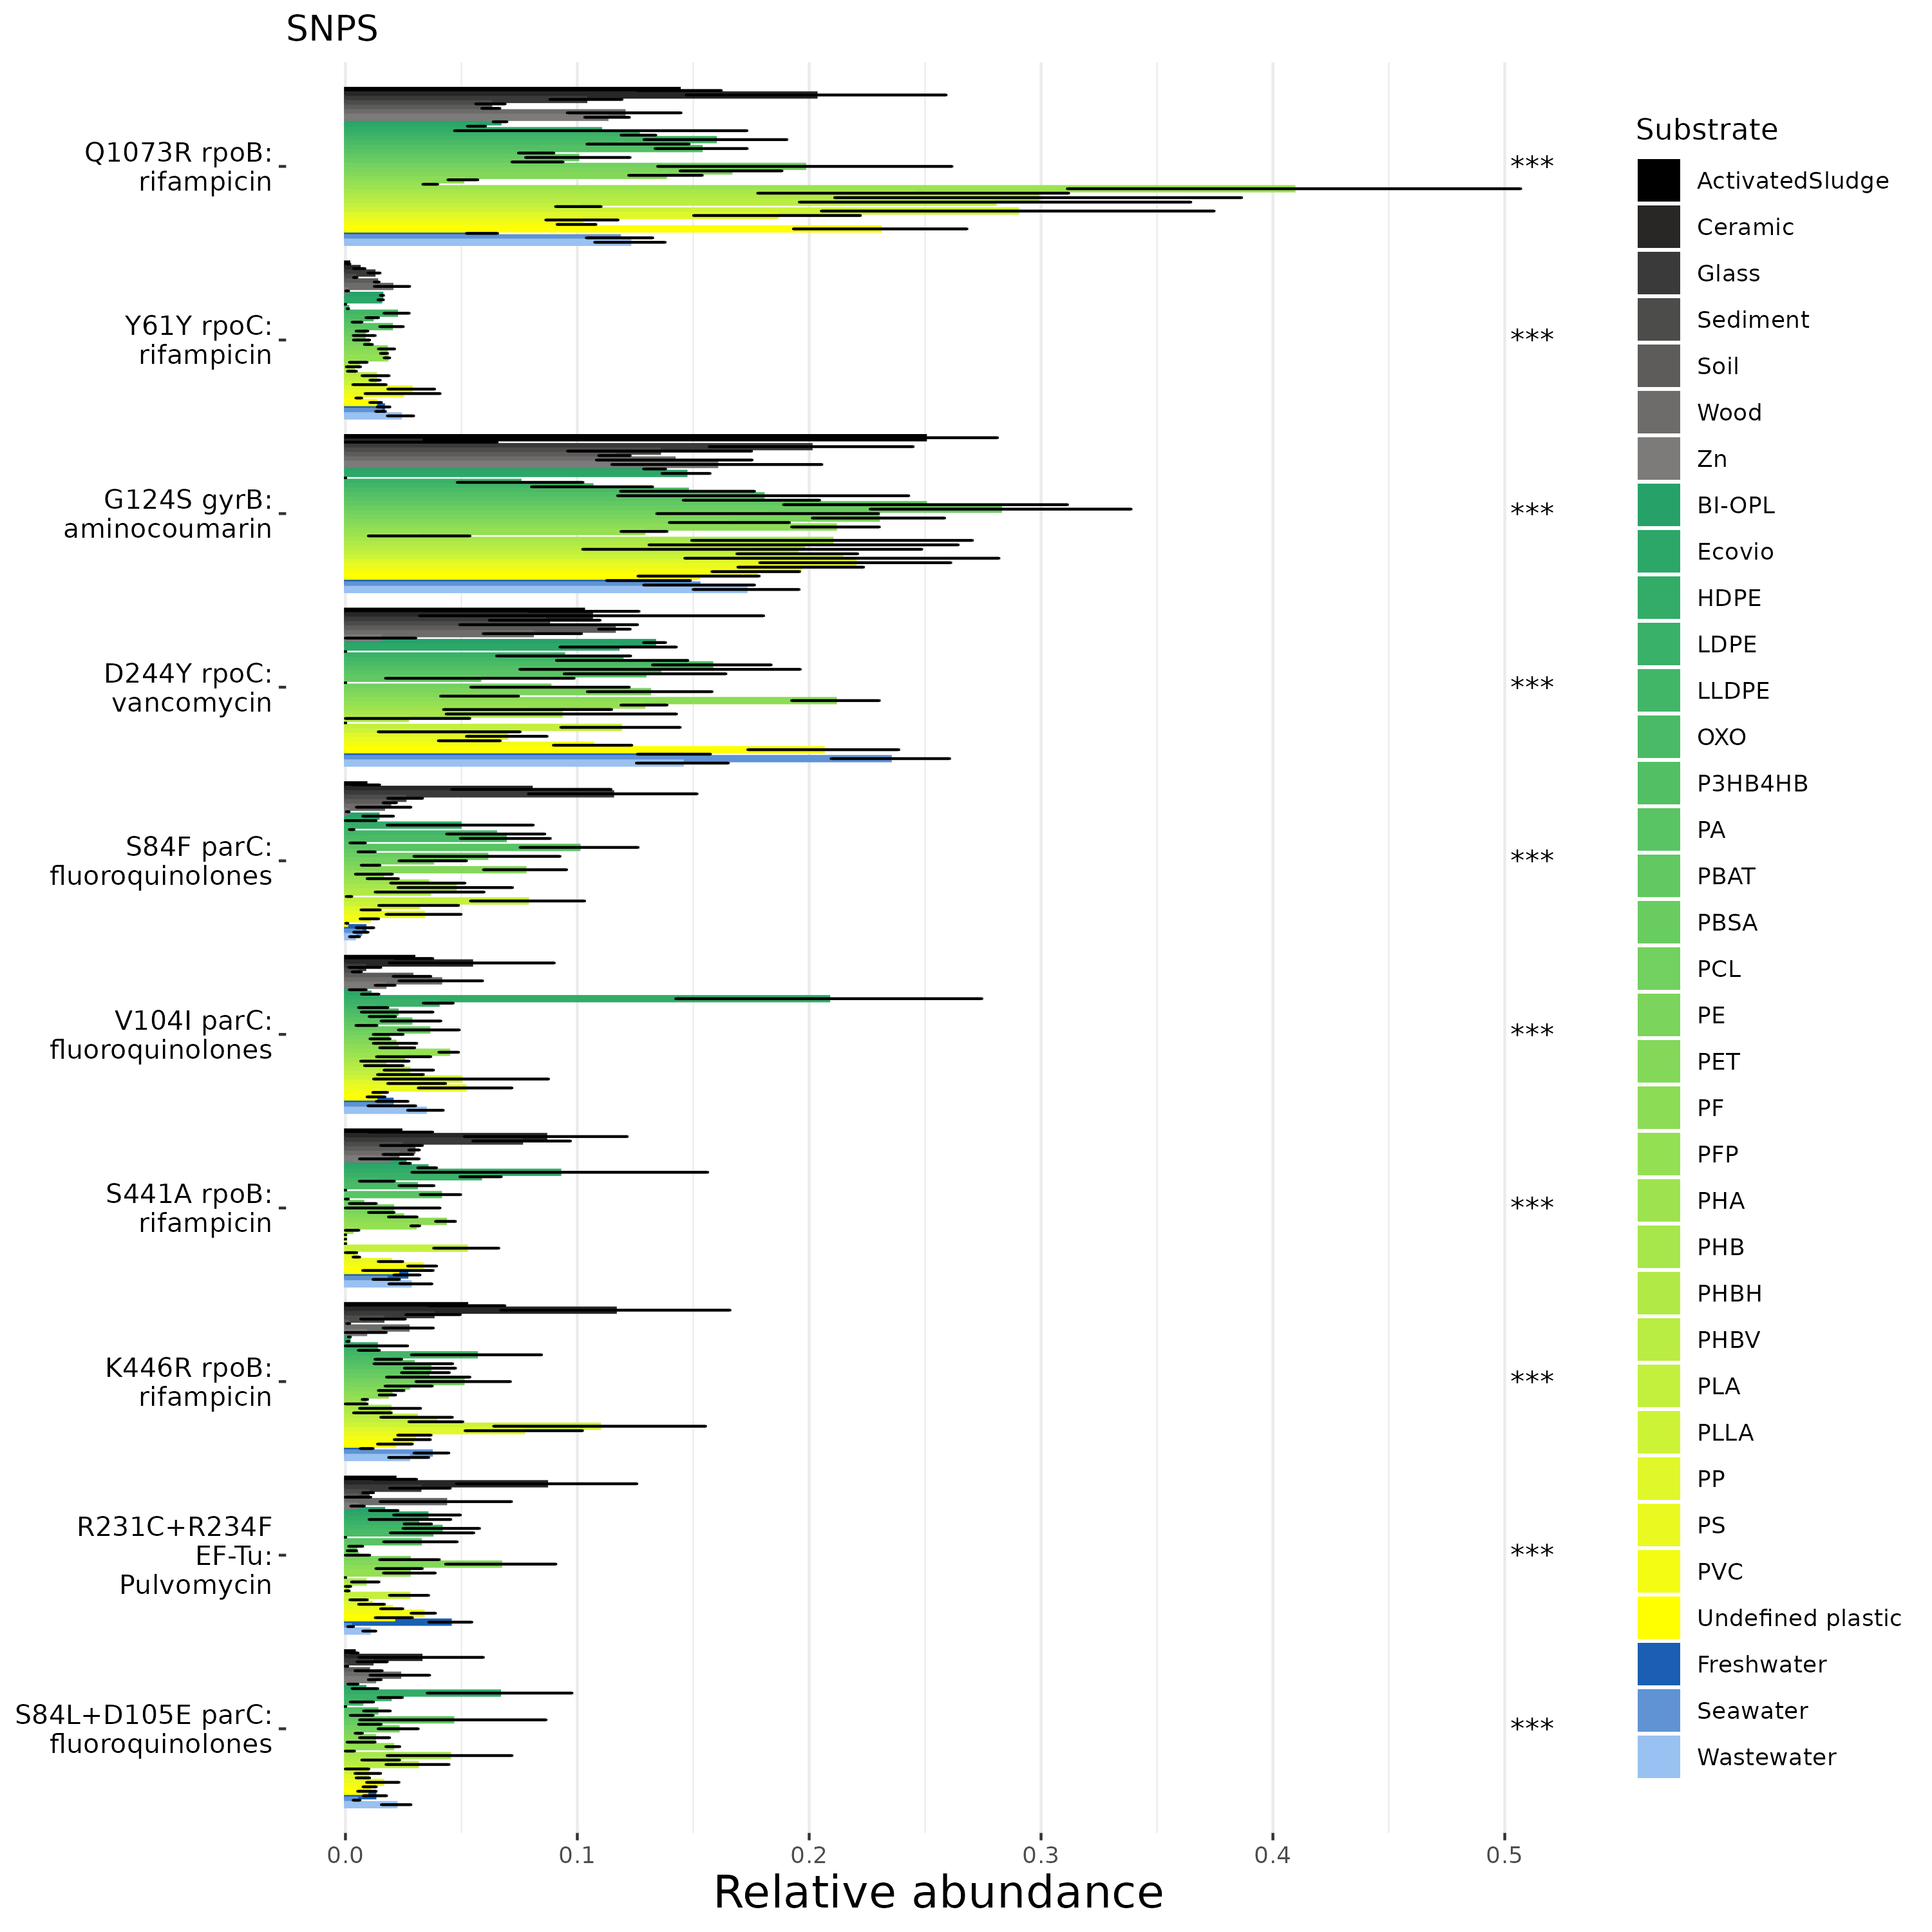
\includegraphics[width=0.5\textwidth]{figure/relative_forest_substrate_snps_abund.png}}
    \caption{(a) Significantly assigned point mutations and Mean Decrease Gini Importance when grouped by substrate. (b) Relative Abundances of the different point mutations in the substrates}
    \label{snps_substrate}
\end{figure}

\section{Taxonomic Composition}
%TODO Show this for the sake of it?
The taxonomic abundance of all samples is shown in figure \ref{tax_plot}. The plot show the taxonomic composition at the phylum level, and is divided by ecosystem type and sampletype. Only the eight most abundant phyla has been included, where the rest has been grouped into "Others".
%The ecosystem type is the environment in which the sample was taken, regardless of the sampletype. For example, some of the samples were taken in the Pacific Ocean, and there both plastic substrates and seawater substrates were analysed.
%The figure shows that the largest difference is between the different ecosystems, but that sampletype also matters.\{Very unsure of how to analuze these plots, since we lack statistics for them.}
The most abundant phyla in all ecosystems are \emph{Proteobacteria}, except in the wastewater samples where SAR is most abundant in most of the samples.
Other abundant phyla are \emph{Archaeplastida} in the PE samples from the Ocean ecosystem, see \ref{tax_plot_substrate_flip}, \emph{Amorphea} in the Undefined palstic samples and in PVC from wastewater. The soil and sediment samples contain a large proportion of Others, into which the phyla not part of the eight most abundant ones are grouped. 

%wastewater: Archaeplastida (Some ocean plastic samples, the PE ones)
%Plastic and wastewater: Amorphea (plastic: undefined, from great pacific garbage patch; wastewater: PVC)
%Soil and sediment: >50\% others

%there are differences between the different ecosystems, but that there is relatively small differences between the different sampletypes and substrates. 

%Figure \ref{tax_plot_substrate} show the same plot, but this time also divided by substrate.\{Which of these should be present? Could turn the whole plot 90° on the page to be easier to read? see fig \ref{tax_plot_substrate_flip}}

\begin{figure}[h]
    \centering
    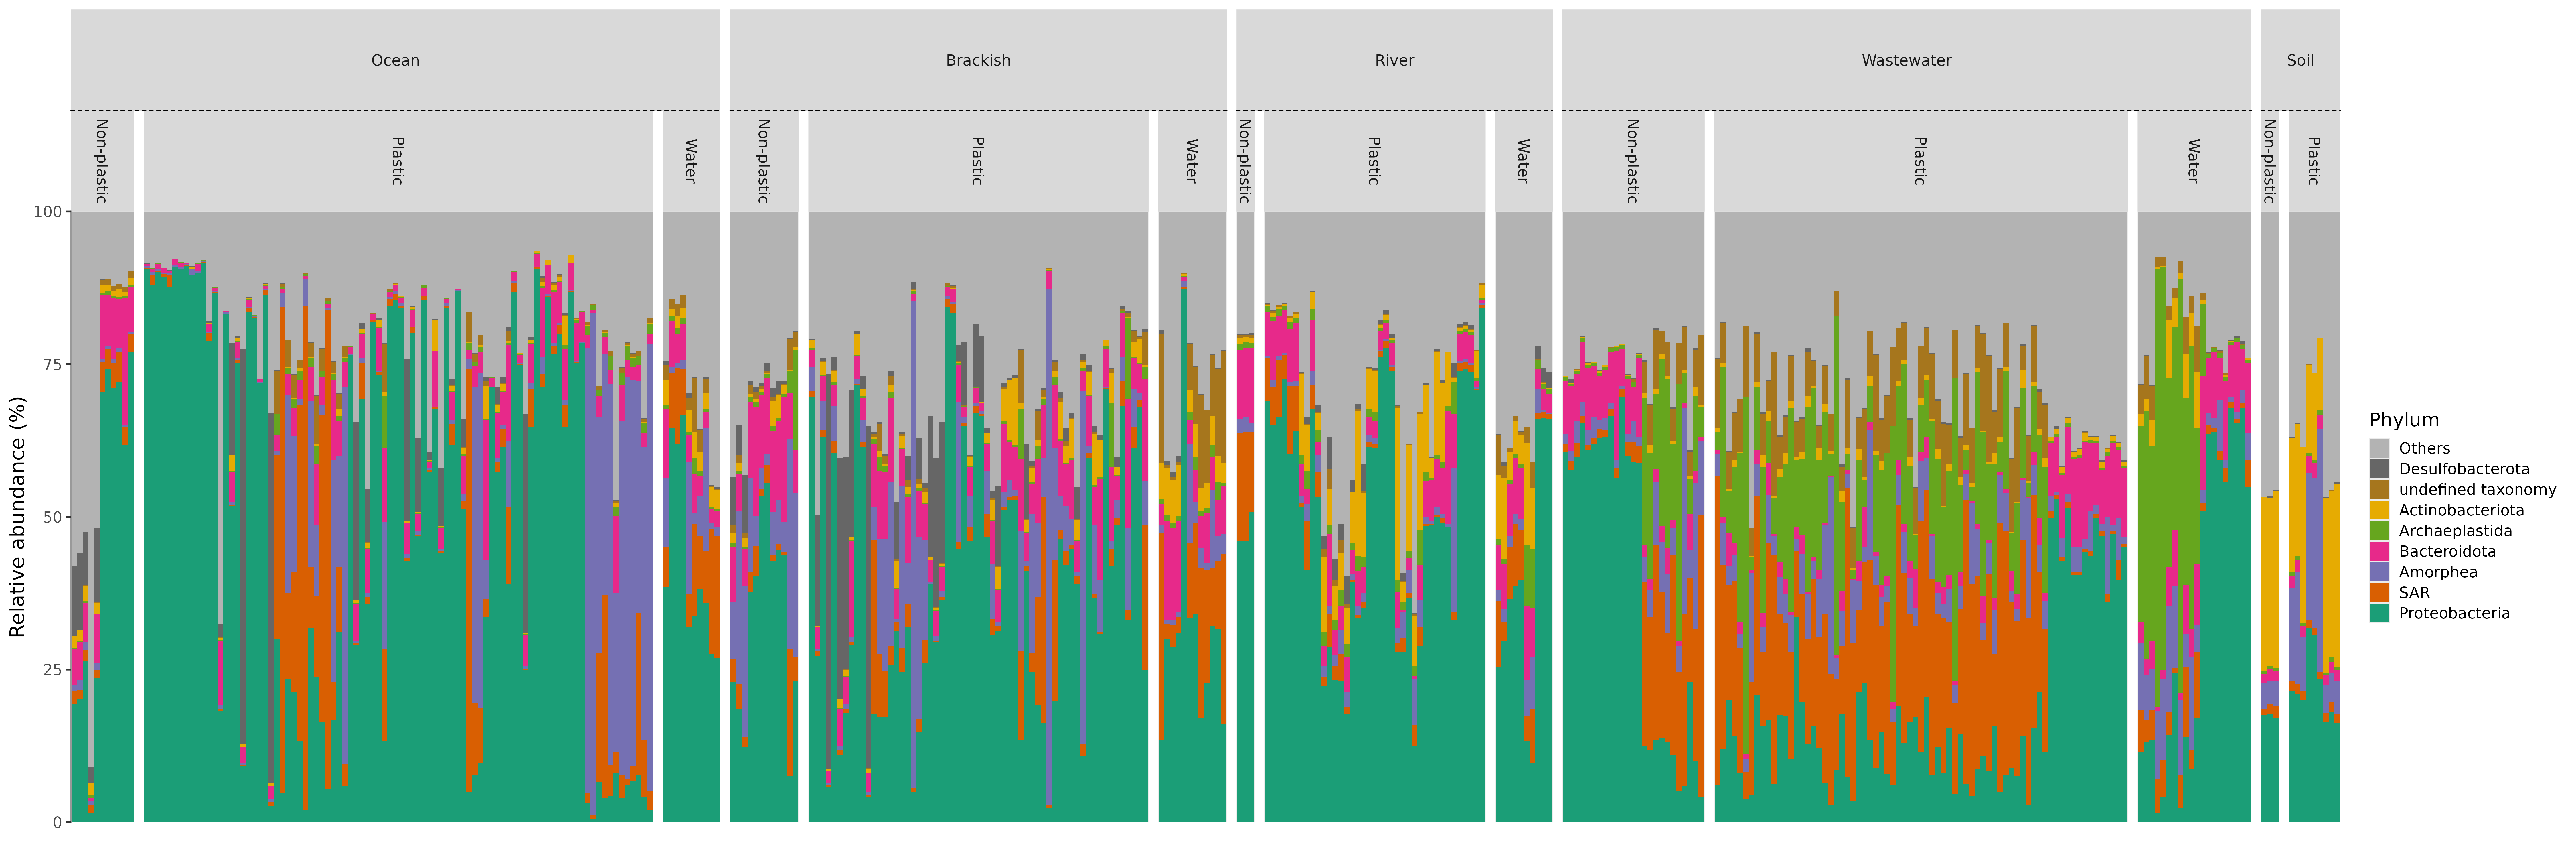
\includegraphics[width = 0.9\textheight, angle = 90]{figure/tax_phylum_ecosystem_sampletype.png}
    \caption{Taxonomic composition for all samples showing the top 8 phyla, divided by ecosystem type and sampletype}
    \label{tax_plot}
\end{figure}














% DISCUSSION
\chapter{Discussion}

% From Máté:
% - Start with a summary of 
%   - what you did
%   - what this project was about
%   - what was the main question
%   - what is you answer to the main question
% - Then you could add a one-one key sentence from each important result section. 
% - Thereafter you "zoom in" and elaborate more for all the sentences that you summarized in 
%   the first paragraph.
%   - And discuss your results, compare them with other findings, state whether the findings were surprising or not, if so, what could explain your observed patterns.
% (also present below)

% - No need to refer to figures in the discussion

% ----- 
% Aim
The aim of the study was to identify specific point mutations in the plastisphere which can lead to altered susceptibility of microorganisms to antibiotics. 
In addition to this the levels of these specific point mutations were to be compared with those in microorganisms which inhabit water or natural substrates.
% Method
To achieve this the point mutations present in samples from 35 different substrates were obtained, in addition to the amount of reads which map to each specific point mutation. 

% Main point
Overall, the results suggest that plastics in general does not increase the prevalence of specific point mutations in microbes in the plastisphere in comparison to those living in planktonic forms in the surrounding water.
However, specific plastic substrates such as PVC, PFP, Ecovio, and BI-OPL increased the relative mutation percentage in the sample.
The antibiotics with the highest mutation percentage were rifampicin, aminocoumarin, vancomycin, and fluoroquinolones.

The presence of certain genes and gene families were successful in indicating sample origin and substrate type.
These include fluoroquinolone resistant parC (HDPE) and rifamycin resistant ropB (PHA) for the gene families and G124S gyrB (aminocoumarin resistance, PBSA), V104I or S84L+D105E parC (fluoroquinolone resistance, PFP), and Q1073R rpoB (rifampicin resistance, PHBV) for the point mutations.
In other words, these genes are more prone to experience point mutations, leading to antibiotic resistance to fluoroquinolone, rifamycin, aminocoumarin, and rifampcin.

% Zoom in and other studies
Previous studies found that the biofilm on microplastics enrich ARGs compared to the surrounding water \cite{zhou2024MicroplasticBiofilmsPromote}, and that this biofilm is distinct from the microbiome of the surrounding water \cite{zadjelovic2023MicrobialHitchhikersHarbouring}. 
% READ PER MILLION
In our study however, there was a higher amount of point mutations in the water samples than the plastic samples, and the freshwater samples had a significantly higher mean than most other substrates. 
The cause of this could be that the main driving force for the accumulation of ARGs in the plastisphere being horizontal gene transfer, and not mutation-induced resistance development, as shown by previous studies \cite{goswami2025MicroplasticsHiddenDrivers} which would explain the relationship we observe.
However, when the amount of point mutations present in different substrates were compared there were plastic substrates (PFP, Ecovio, BI-OPL, PHB, PF, PBAT and LDPE) with more mutations than the water substrates.
This signifies that there are plastic substrates which do increase the prevalence of specific point mutations, which correlates well with the results from Li et al. \cite{li2021ImpactUrbanizationAntibiotic}, which found the amount of ARGs to vary between microplastic substrates. The authors also found that PE had the highest enrichment of aminoglycoside resistance genes, a mutation present in the plastisphere of all the substrates they used.
Some of the plastics we found which increase the amount of point mutations were PFP (PE-fiber-PE), PF (PE-fiber), and LDPE (low-density PE), all of which consists of PE (polyethylene). 
%They also found there to be a significant (p < 0.01) correlation between specific surface area and the abundance of ARGs, which could explain the differences between substrates, however this effect warrants further study. 
% Stevenson et al. \cite{stevenson2024SelectionAntimicrobialResistance} found that different plastic substrates enrich bacteria to different levels, where especially PS particles enrich AMR bacteria. 

% SAMPLES
When instead considering the mean mutation percentage among the samples, the mean mutation percentages was generally lower in the plastisphere than in the surrounding microbial communities.
However, this comparison also showed differences between the substrates, where PVC, PFP, LDPE, Ecovio, and BI-OPL had higher mean mutation percentage than seawater or wastewater. 

% POINT MUTATIONS
When the mean mutation rate of the individual point mutations were compared between the plastic and water group, the plastic group had a higher mean than the water group. 
This is because the plastic samples contained many mutations at low mutation frequencies which the water samples did not, and therefore reduced the mean of the water samples accordingly since these had a mutation rate of zero in the water samples.
This nonspecific increase in mutation frequency could be due to an increase of oxidative stress caused by the pollutants accumulated in the particles or additives released by them \cite{forero-lopez2022PlastisphereMicroplasticsSitu, carvajal-garcia2023OxidativeStressDrives}. In the previous studies, these pollutants included chromium and zinc, and the additives included pigments such as titanium dioxide, and lead(II) chromate \cite{liu2020EffectAgingAdsorption}.

Since it was possible to predict the identity of the substrate to which a sample belonged using specific point mutations or AMR gene families, there was a difference between the different substrates in respect to these. 
However, since one cannot predict association to the plastic group there are no point mutations or AMR gene families which define the plastisphere clearly, highlighting the importance of defining specific substrates when comparing the results of different studies of the plastisphere. 
%The point mutations which may be used to predict identity were present in gyrB, parC and rpoB, all of which 
This result also show there being some substrates which show an increase in specific point mutations, while there is not evidence for the same for the plastic group as a whole.

% The random forest analysis show that there are both AMR Gene Families and point mutations that are significant and may be used to predict the identify of specific substrates, however one cannot predict group association other than to the non-plastic group.

Several of the plastic substrates are biodegradable including BI-OPL, Ecovio, PBAT, PHA, PHB, PHBV, and PLA. Liu et al. \cite{liu2023EffectsComparisonSecondary} show that biodegradable plastics promote the transfer of ARGs between bacteria, however there are no studies that shown an increase in point mutation in them, highlighting another area of further study.

One must take care when interpreting these results, since the mutations identified all come from a single database, which cannot be assumed to be complete. Further studies could use other databases to raise the confidence of the specific mutations found herein. 
Further consideration must also be taken for the clinical relevance of these findings, since the clinical efficacy of the antibiotic resistance is not known, and is only based on presumed conferral of antibiotic resistance, based on the presence of the point mutation in the genome of the pathogen.

The overall result of the current study therefore reject the original hypothesis, there is not an increase in the prevalence of specific point mutations conferring antibiotic resistance in microbes in the plastisphere in comparison to those living in planktonic forms in the surrounding water. However, specific plastic substrates do increase the prevalence of point mutations in the plastisphere, and is an area which warrant further studies. 

% TODO: Most common plastics? -> Theory?

% Obsidian-text: -----------------
%Good Paragraph! 
%Move sentences around and place them in line with your specific findings!
% Previous studies found that the biofilm on microplastics enrich ARGs compared to the surrounding water \cite{zhou2024MicroplasticBiofilmsPromote}, and that this biofilm is distinct from the microbiome of the surrounding water \cite{zadjelovic2023MicrobialHitchhikersHarbouring}. 
    % Stevenson et al. \cite{stevenson2024SelectionAntimicrobialResistance} show that particularly microplastic particles of PS enrich AMR bacteria compared to non-plastic materials such as wood and glass. This falls in line with the result that different plastic substrates behave differently, altough the specific substrate in question was different.% between that study and this one.
%The main driving factor for the accumulation of ARGs in the plastisphere is horizontal gene transfer (HGT) \cite{goswami2025MicroplasticsHiddenDrivers} between microorganisms, and not mutation-induced resistance development.
% This could reduce the selective pressure for point mutations, therefore reducing the amount of them that are present. 
% This could also explain the result of non-selective increase of point mutations, where environmental stresses increase the amount of point mutations non-selectively.
    %Therefore, although the plastisphere selects for AMR-carrying bacteria, the method through which this resistance occur is not, in general, through specific point mutations caused by the plastic substrate.
%The small non-specific increase of point mutations on the plastic substrates could instead be due to oxidative stress caused by the pollutants accumulated in the particles or additives released by them \cite{forero-lopez2022PlastisphereMicroplasticsSitu, carvajal-garcia2023OxidativeStressDrives}.

% From theory:
    %Compared to bacteria in the surroundig water, the rate of gene transfer increased by 7.2-19.6 times \cite{zhou2024MicroplasticBiofilmsPromote} in the plastisphere. Of the tested microplastics in the study, Zhou et al. found that the biofilm formed on polyethylene (PE) plastic had the highest conjugation rate as well as bacterial density. 


% ----- 
% One needs to be aware however that a high mean decrease of Gini impurity does not mean that the mutation or AMR gene family has a higher abundance in the corresponding substrate, but only that the variable can be used to differentiate it. The actual abundance may be higher or lower than the reference group, the other substrates, but it does differ from the other substrates. 
% It can also vary more or less than the reference? Find better reference to refer to

% the antibiotics in 22 resistances:
% - fluoroquinolones
% - rifampicin
% - isoniazid
% - pulvomycin
% - rifabutin
% - enacyloxin iia
% - aminocoumarin
% - fosfomycin
% - vancomycin
% - fusidic acid
% 
% genes: 
% - parC
% - gyrA
% - gyrB
% - rpoB
% - katG
% - EF-Tu
% - parE
% - ponA1
% - soxS
% - UhpT
% - rpoC
% - fusA

% --------------
% Intressant för senare:
% Metagenome Assemeled Genomes - MAG, linking ARGs and other virulence-related genes to their host.
% - Escheria coli harboured more ARGs and virulence factors than any other MAG
% --------------
% HDPE, PBSAA, PHA for AMR Gene Families
% PBSA, PFP, PHBV for point mutations











% CONCLUSION
% CREATED BY MAGNUS GUSTAVER, 2020
\chapter{Conclusion}

%By analysing the number of point mutations which confer antiobiotic resistance, the result of which is shown in figure \ref{hits_type} and \ref{hits_substrate}, one may conclude that the number of point mutations which confer antibiotic resistance are not more prevalent on all plastics, but instead that specific plastic substrates increase this count.
%These substrates include PFP, Ecovio, and BI-OPL. The latter two are biodegradable plastics which contain a blend of PBAT and PLA. 
\begin{itemize}
    \item Plastics as a group does not increase the mean mutation percentage of the sample significantly, but specific plastic substrates do.
    \item When calculating the mean mutation percentage for mutations, grouped by sampletype or substrate, the plastic samples show a significant increase compared to the other two groups. Since the tests are paired, I think this means that more mutations have a higher mean mutation percentage in the plastic samples than the water samples?
    \item The two above results mean that there are more mutations/hits on the water samples, the total sum is higher from some few which are higher, but that there is a small increase in many different mutations in plastic samples, and therefore they are significant and higher when testing in the second way.
    \item Random forest shows there are different mutations on different substrates, can distinguish between them.
\end{itemize}


% REFERENCES / BIBLIOGRAPHY
\cleardoublepage
\addcontentsline{toc}{chapter}{Bibliography}
%% CREATED BY MAGNUS GUSTAVER, 2020
\begin{thebibliography}{69}

\bibitem{Reference} Gustaver, M. (2020) A Chalmers University of Technology Master's thesis template for \LaTeX . Unpublished.

\end{thebibliography}

% Från en gammal labbrapport:
%\newpage
%\addcontentsline{toc}{section}{References}
\bibliographystyle{IEEEtran}
\bibliography{references}

% APPENDICES
\cleardoublepage
\appendix
\setcounter{page}{1}
\pagenumbering{Roman}			% Capitalized roman numbering starting from I (one)

% CREATED BY MAGNUS GUSTAVER, 2020
\chapter{Appendix 1}
\label{appendix:studies}
\todo{Insert table with references to studies}
% Format: ENA_accession - Name - Authors - Reference ?


\chapter{Appendix 2}
%\renewcommand{\arraystretch}{1.2}
\todo{Split table to next page or decrease size of it in some way?}


\begin{table}[H]
\caption{Number of samples for each substrate type}
\label{substrate_sampletype}
\begin{tabular}{@{}lll@{}}
\toprule
\textbf{Sampletype}           & \textbf{Substrate} & \textbf{Samples} \\ \midrule
\multirow{26}{*}{Plastic}     & BI-OPL             & 3          \\
                              & Ecovio             & 3          \\
                              & HDPE               & 11         \\
                              & LDPE               & 6          \\
                              & LLDPE              & 12         \\
                              & OXO                & 11         \\
                              & P3HB4HB            & 5          \\
                              & PA                 & 12         \\
                              & PBAT               & 5          \\
                              & PBSA               & 5          \\
                              & PCL                & 8          \\
                              & PE                 & 29         \\
                              & PET                & 19         \\
                              & PF                 & 5          \\
                              & PFP                & 5          \\
                              & PHA                & 8          \\
                              & PHB                & 5          \\
                              & PHBH               & 5          \\
                              & PHBV               & 5          \\
                              & PLA                & 15         \\
                              & PLLA               & 5          \\
                              & PMMA               & 1          \\
                              & PP                 & 18         \\
                              & PS                 & 19         \\
                              & PVC                & 28         \\
                              & Undefined plastic  & 24         \\ \midrule
\multirow{3}{*}{Water}        & Freshwater         & 11         \\
                              & Seawater           & 21         \\
                              & Wastewater         & 20         \\
\multirow{10}{*}{Non-plastic} & ActivatedSludge    & 14         \\ \midrule
                              & Cardboard          & 1          \\
                              & Ceramic            & 3          \\
                              & Glass              & 11         \\
                              & Leaf               & 1          \\
                              & Rock               & 1          \\
                              & Sediment           & 5          \\
                              & Soil               & 3          \\
                              & Wood               & 12         \\
                              & Zn                 & 6          \\ \bottomrule
\end{tabular}
\end{table}


% CREATED BY MAGNUS GUSTAVER, 2020
\newpage

%Header Last Page
\vtop{
    \null\vspace{-47.5mm}
    \centerline{\textcolor{thesisHeaderColor}{\rule{1.28\textwidth}{28mm}}}
    \null\vspace{-9mm}
    \centerline{\textcolor{headerBrown}{\rule{1.28\textwidth}{4pt}}}
}

\addtolength{\voffset}{2cm}
\renewcommand{\familydefault}{\sfdefault} \normalfont % Set cover page font
\pagestyle{empty}
\vspace*{-4.5cm}
\noindent
\textcolor{white}{\footnotesize \textbf{DEPARTMENT OF SOME SUBJECT OR TECHNOLOGY}\\
\textbf{CHALMERS UNIVERSITY OF TECHNOLOGY} \\
Gothenburg, Sweden \\
\href{www.chalmers.se}{\textcolor{white}{www.chalmers.se}}}


\vfill
\if\InstitutionLocation C   %Defined in settings.tex
\centerline{
\includegraphics[width=0.2\pdfpagewidth]{figure/auxiliary/AvancezChalmersU_black_centered.eps}}
\fi
\if\InstitutionLocation G
\centerline{
\includegraphics[width=0.3\pdfpagewidth]{figure/auxiliary/chalmers_gu_black_centered_eng.eps}}
\fi
\vspace{14mm}

\end{document}
